%%%%%%%%%%%%%%%%%%%%%%%%%%%HEADER%%%%%%%%%%%%%%%%%%%%%%%%%%%%%%
%%%%%%%%%%%%%%%%%%%%%%%%%%%HEADER%%%%%%%%%%%%%%%%%%%%%%%%%%%%%%
%%%%%%%%%%%%%%%%%%%%%%%%%%%HEADER%%%%%%%%%%%%%%%%%%%%%%%%%%%%%%
%Note: All the options like chapterprefix, pointednumbers, etc affect the way things are represented in the header of each page
\documentclass[a4paper,11pt,listof=nochaptergap,oneside,pointednumbers,bibtotoc,bigheadings,liststotoc]{scrbook}
% note that the option 'listof=nochaptergap' disables the chapter separation in listoffigures and listoftables!
% note that the expression "numbers=noenddot" remoes the dot after the number in figure captions
% for details see https://tex.stackexchange.com/questions/27250/remove-dot-after-number-in-figure-captions-while-keeping-the-dot-in-chapter-sect
\usepackage[utf8]{inputenc} %für Umlaute etc.
\usepackage[T1]{fontenc}
\usepackage[ngerman, english]{babel} %English titles (figure, table) und englische Silbentrennung
\usepackage{a4wide}
\usepackage{parskip} %see https://golatex.de/wiki/%5Cparskip to know what the package can do
\usepackage[pdftex]{color}
\usepackage{lmodern} \normalfont %to load T1lmr.fd  %weniger verpixelte Schrift; mehr Infos: http://www.namsu.de/Extra/pakete/Lmodern.html
%den genauen Trick für die untere Zeile kann ich hier nochmal nachlesen: http://tex.stackexchange.com/questions/22240/choosing-font-for-bold-small-caps-or-any-other-particular-familyseriesshape-c
\DeclareFontShape{T1}{lmr}{bx}{sc} { <-> ssub * cmr/bx/sc }{} 
\usepackage{a4} %anscheinend besser hier die Formatierung a4 wählen als als Option von documentclass
\usepackage[colorlinks = true,
		     bookmarks, 
		     linkcolor = red,
		     urlcolor = blue]{hyperref}
%\usepackage{fancyhdr}
\usepackage[right]{eurosym}
% the below two lines of code are necessary to make sure that the numbering of figures starts at 1 and then proceeds in steps of 1 instead of floating point numbers etc.
\usepackage{chngcntr}
% the below package is useful to be able to properly write down the indicator function!
\usepackage{bbm}
% lscape is to be able to put a table in landscape mode
\usepackage{lscape}
% the below is ncessary to let the footnote numbering continue over pages and chapters
\usepackage{chngcntr}
\counterwithout{footnote}{chapter}
% the below is necessary to be able to align a table by decimal points
\usepackage{dcolumn,booktabs}
\newcolumntype{d}[1]{D{.}{.}{#1}}
%\newcommand\mc[1]{\multicolumn{1}{c}{#1}} % handy shortcut macro
% the footmisc package allows multiple footnotes separated by a comma
\usepackage[multiple]{footmisc}
% the below package is necessary to be able to include in-table footnotes and make them
% show up at the bottom of the page instead of below the table
\usepackage{tablefootnote}
% package to be able to use 'bm' for boldface
\usepackage{bm}
% longtable is to be able to break a table across multiple pages
\usepackage{longtable}
\counterwithout{figure}{chapter}
\counterwithout{table}{chapter}
% the below code allows the adjustment 

\usepackage{amsmath, amssymb, amstext} %für Mathematik
\usepackage{mathstyle} %mehr Infos: http://www.ctan.org/pkg/mathstyle
\usepackage{blindtext} %to be able to place blindtext at certain locations
\usepackage[left=35mm, right=35mm, top=50mm, bottom=35mm]{geometry}%Seitenränder anpassen
\usepackage[onehalfspacing]{setspace} %1.5 Zeilgenabstand
\usepackage[round, comma]{natbib} %für die Bibliographie
%all four of the below packages are included for table creation
\usepackage{booktabs} 
\usepackage{array}
% we define new column types that take their width as argument and do
\newcolumntype{L}[1]{>{\raggedright\let\newline\\\arraybackslash\hspace{0pt}}m{#1}}
\newcolumntype{C}[1]{>{\centering\let\newline\\\arraybackslash\hspace{0pt}}m{#1}}
\newcolumntype{R}[1]{>{\raggedleft\let\newline\\\arraybackslash\hspace{0pt}}m{#1}}

\usepackage{multirow}
\usepackage{tabularx}
\usepackage{lscape}
\usepackage{mathstyle} %mehr Infos: http://www.ctan.org/pkg/mathstyle
\usepackage[pdftex]{graphicx} %to include graphics
\usepackage{microtype} % makes pdf look better
\usepackage{booktabs}
%the below package allows the modification of the enumeration symbols
\usepackage{enumerate}% http://ctan.org/pkg/enumerate
\usepackage{dcolumn} % Ausrichtung nach Dezimalpunkt in Tabellen
\newcolumntype{.}{D{.}{.}{-1}}
\usepackage{setspace}
\pagestyle{headings}
% the below code is necessary to be able to customize the font of the Figure caption for figures
\usepackage{caption} % see https://www.namsu.de/Extra/pakete/Caption.html for more information!
\captionsetup[table]{font=scriptsize,labelfont=footnotesize,labelfont=bf, singlelinecheck = false, format=hang, justification=justified, skip=10pt}
\captionsetup[figure]{font=scriptsize,labelfont=footnotesize,labelfont=bf, singlelinecheck = false, format=plain, justification=justified}%width=\dimexpr\textwidth-2cm\relax}
%\setlength{\textwidth}{15cm}
%\setlength{\textheight}{22.5cm}
%\setlength{\oddsidemargin}{1cm}
%\setlength{\evensidemargin}{0cm}
% \renewcommand{\baselinestretch}{1.2}
% \parskip1ex plus0.5ex minus0.5ex
%um die Überschriften im Inhaltsverzeichnis anzupassen
\usepackage{tocloft}
\renewcommand{\cftchapaftersnum}{.} %add period after the chapter number in ToC
% see https://tex.stackexchange.com/questions/411708/add-period-in-list-of-figures-list-of-tables
\renewcommand{\cftfigaftersnum}{.} %add period after figure number in list of figures
\renewcommand{\cfttabaftersnum}{.} %add period after table number in list of tables
\renewcommand\cftchapfont{\large\bfseries}%changes font and fontsize of chapters in toc
%\renewcommand\cftsecfont{\normalsize}
\renewcommand{\cfttoctitlefont}{\LARGE\bfseries}	%changes font of 'Content' header before toc
\renewcommand{\cftloftitlefont}{\LARGE\bfseries} %changes font of 'List of Figures'
\renewcommand{\cftlottitlefont}{\LARGE\bfseries} %changes font of 'List of Tables'
% the below commands move the beginning of toc, list of figures and list of tables further down 
% the page
\renewcommand\cftbeforetoctitleskip{2.7cm}
\renewcommand\cftbeforeloftitleskip{2.7cm}
\renewcommand\cftbeforelottitleskip{2.7cm}
%um die Überschriften im Text anzupassen
\usepackage{titlesec}
%der folgende Befehl ändert die Schriftart des "chapter"-Befehls
\titleformat{\chapter}{\large\bfseries\filright}{\LARGE\thechapter.}{15pt}{\LARGE}
\titleformat*{\section}{\large\bfseries}
\titleformat*{\subsection}{\normalsize\bfseries}
\titleformat*{\subsubsection}{\large\bfseries}
\titleformat*{\paragraph}{\small\bfseries}
% the below command is used to adjust the font-size of in-text block quotations
\usepackage{lipsum}% http://ctan.org/pkg/lipsum
\renewenvironment{quote}
               {\list{}{\rightmargin\leftmargin}%
                \item\relax\scriptsize\textquotedblleft\ignorespaces}
               {\unskip\unskip\textquotedblright\endlist}

%---------------------------------------------------------------------- Customizations ---------------------------------------------------------------------
%--------------------------------
%--------------------------------the entire below part is necessary to be able to have a 'Definition'-environment like in Math scripts.
%--------------------------------
\usepackage{amsthm}
\usepackage{amsthm}
\makeatletter
\newtheoremstyle{mysatz} %<name>
  {}% <Space above>
  {}% <Space below>
  {}% <Body font>
  {}% <Indent amount>
  {\bfseries}% <Theorem head font>
  {.}% <Punctuation after theorem head>
  {.5em}% <Space after theorem heading>
  {\thmname{#1}\thmnumber{\@ifnotempty{#1}{ }#2}%
   \thmnote{ {\the\thm@notefont(#3)}}}% <Theorem head spec (can be left empty, meaning `normal')>
\makeatother
%\theoremstyle{definition} %damit der Text innerhalb der Definition 
%nicht kursiv geschrieben wird
\makeatletter
\def\th@mysatz{%
  \thm@notefont{\bfseries}% same as heading font
}
\makeatother

\theoremstyle{mysatz}
\newtheorem{satz}{Satz}[chapter]

\newtheorem{lem}[satz]{Lemma}


\makeatletter
\newtheoremstyle{mydefinition} %<name>
  {}% <Space above>
  {}% <Space below>
  {}% <Body font>
  {}% <Indent amount>
  {\bfseries}% <Theorem head font>
  {.}% <Punctuation after theorem head>
  {.5em}% <Space after theorem heading>
  {\thmname{#1}\thmnumber{\@ifnotempty{#1}{ }#2}%
   \thmnote{ {\the\thm@notefont(#3)}}}% <Theorem head spec (can be left empty, meaning `normal')>
\makeatother
%\theoremstyle{definition} %damit der Text innerhalb der Definition 
%nicht kursiv geschrieben wird
\makeatletter
\def\th@mydefinition{%
  \thm@notefont{\bfseries}% same as heading font
}
\makeatother


\theoremstyle{mydefinition}
\newtheorem{defi}[satz]{Definition}

%\theoremstyle{remark} %damit der Text innerhalb der Bemerkung nicht
%kursiv geschrieben wird
\makeatletter
\newtheoremstyle{mybemerkung} %<name>
  {}% <Space above>
  {}% <Space below>
  {}% <Body font>
  {}% <Indent amount>
  {\itshape}% <Theorem head font>
  {.}% <Punctuation after theorem head>
  {.5em}% <Space after theorem heading>
  {\thmname{#1}\thmnumber{\@ifnotempty{#1}{ }#2}%
   \thmnote{ {\the\thm@notefont(#3)}}}% <Theorem head spec (can be left empty, meaning `normal')>
\makeatother

\theoremstyle{mybemerkung}
\newtheorem{bem}[satz]{Bemerkung}


\renewcommand{\labelitemi}{$\rhd$}



%--------------------------------
%--------------------------------the entire below part is necessary to be able to include an abstract with the books document class
%--------------------------------
\usepackage{lipsum}
\newcommand\abstractname{Abstract}  %%% here
\makeatletter
\if@titlepage
  \newenvironment{abstract}{%
      \titlepage
      \null\vfil
      \@beginparpenalty\@lowpenalty
      \begin{center}%
        \bfseries \abstractname
        \@endparpenalty\@M
      \end{center}}%
     {\par\vfil\null\endtitlepage}
\else
  \newenvironment{abstract}{%
      \if@twocolumn
        \section*{\abstractname}%
      \else
        \small
        \begin{center}%
          {\bfseries \abstractname\vspace{-.5em}\vspace{\z@}}%
        \end{center}%
        \quotation
      \fi}
      {\if@twocolumn\else\endquotation\fi}
\fi
\makeatother

%--------------------------------
%--------------------------------the entire below part is necessary to be able to customize the header
%--------------------------------

\usepackage{fancyhdr} %Paket für Kopf- und Fußzeile laden
\setlength{\headheight}{15.2pt}
\pagestyle{fancy} %wir aktivieren unseren eigenen Seitenstil
%der folgende Befehl ändert die Schriftart im Header:
\renewcommand{\chaptermark}[1]{\markboth{\chaptername\  
\thechapter. \textit{#1}}{}}
\fancyhf{} %alle Kopf- und Fußzeilenfelder bereinigen
\fancyhead[R]{\thepage}
\fancyhead[L]{\rightmark}
\renewcommand{\headrulewidth}{0.4pt} %customizing obere Trennlinie

%% a bunch of code to control the length of the headrule
%% Length to control the \fancyheadoffset and the calculation of \headline
%% simultaneously
%\newlength\FHoffset
%\setlength\FHoffset{0cm}
%
%\addtolength\headwidth{2\FHoffset}
%
%\fancyheadoffset{\FHoffset}
%
%% these lengths will control the headrule trimming to the left and right 
%\newlength\FHleft
%\newlength\FHright
%
%% here the trimmings are controlled by the user
%\setlength\FHleft{0cm}
%\setlength\FHright{0cm}
%
%% The new definition of headrule that will take into acount the trimming(s)
%\newbox\FHline
%\setbox\FHline=\hbox{\hsize=\paperwidth%
%  \hspace*{\FHleft}%
%  \rule{\dimexpr\headwidth-\FHleft-\FHright\relax}{\headrulewidth}\hspace*{\FHright}%
%}
%\renewcommand\headrule{\vskip-.7\baselineskip\copy\FHline}
%% above is a bunch of code to control the length of the headrule

% the below code creates the opportunity to include a quote at the beginning of a chapter
% customize chapter format:
\KOMAoption{headings}{twolinechapter}
\renewcommand*\chapterformat{\thechapter\autodot}

% add chapter quote to beginning of chatpers
% see https://tex.stackexchange.com/questions/53377/inspirational-quote-at-start-of-chapter
\makeatletter
\renewcommand{\@chapapp}{}% Not necessary...
\newenvironment{chapquote}[2][2em]
  {\setlength{\@tempdima}{#1}%
   \def\chapquote@author{#2}%
   \parshape 1 \@tempdima \dimexpr\textwidth-2\@tempdima\relax%
   \itshape}
  {\par\normalfont\hfill--\ \chapquote@author\hspace*{\@tempdima}\par\bigskip}
\makeatother

\newcommand\textbox[1]{%
  \parbox{.333\textwidth}{#1}%
}

%--------------------------------
%--------------------------------additional customizations
%--------------------------------
\setlength{\parindent}{0pt} %legt die Einrücktiefe der ersten Zeile für alle folgenden Absätze fest
% adds a command for exceptional paragraph identation!
\newcommand{\forceindent}{\leavevmode{\parindent=1em\indent}}
\setlength{\abovecaptionskip}{-15pt plus 3pt minus 2pt} %modify vertical space between figure and caption
\renewcommand*{\paragraph}[1]{\subsubsection*{#1} \vspace{-3mm}} %mit diesem Befehl kann man ganz einfach
%PARAGRAPH eingeben und latex macht sofort eine subsubsection ohne Nummerierung usw draus
%customizations für Vektoren (dass sie bold dargestellt werden anstatt mit einem Vektorpfeil)
\let\oldhat\hat
\renewcommand{\vec}[1]{\bm{#1}}
%\renewcommand{\hat}[1]{\oldhat{\bm{#1}}}

\newcommand{\vect}[1]{\boldsymbol{\mathbf{#1}}}
\newcommand{\hatt}[1]{\oldhat{\boldsymbol{\mathbf{#1}}}}
\newcommand{\hattnobf}[1]{\oldhat{#1}}






%%%%%%%%%%%%%%%%%%%%BEGINNING OF THE DOCUMENT%%%%%%%%%%%%%%%%%%%%%%%%
%%%%%%%%%%%%%%%%%%%%BEGINNING OF THE DOCUMENT%%%%%%%%%%%%%%%%%%%%%%%%
%%%%%%%%%%%%%%%%%%%%BEGINNING OF THE DOCUMENT%%%%%%%%%%%%%%%%%%%%%%%%
\begin{document}
%----------------------------------------------------------- Beginn Titelseite -------------------------------------------------------------------------------
%\changefont{ppl}{m}{n} %mit diesem Befehl kann global ganz leicht die Schriftart geändert werden
\newgeometry{left=30mm, right=30mm, top=0mm, bottom=0mm}
\begin{titlepage}
    \begin{center}
        \hspace*{-0.27\textwidth}
\includegraphics[width=1.419\textwidth, trim = 5mm 250mm 0mm 0mm, clip = TRUE]{logo.pdf}\hspace*{-0.3\textwidth}
        \quad \\[0mm]
        \newcommand{\HRule}{\rule{\linewidth}{0.3mm}} %Befehl zum Erstellen der Linie
        \HRule \\[-1mm]
        \Huge{\scshape\bfseries Time-Varying Uncertainty and Business Cycles} \\[-5mm]
        \HRule \\[2mm]
        \Large {\scshape A Shock Restricted Structural Vector \\
        				Autoregression Approach} \\[10mm]
        \Large Master's Thesis \\[10mm]
        \Large in partial fulfillment of the requirements \\for the degree of Master of Science (M.Sc.)\\
                  in Applied Economics \\[10mm]
                  
        submitted to\\
        Univ.-Prof. Dr. Johann Scharler \\[10mm]
        Department of Economics\\
        Faculty of Economics and Statistics\\
        Leopold-Franzens-Universität Innsbruck \\[10mm]
        by \\ Mag. Marcel A. Kropp \\[10mm]
        Innsbruck, July 2018
    \end{center}
\end{titlepage}

%----------------------------------------------------------- Ende Titelseite -------------------------------------------------------------------------------
\restoregeometry

%----------------------------------------------------------- Beginn Widmung Mum ---------------------------------------------------------------------
%Kurze Widmung an Mum.
\thispagestyle{empty} %bewirkt, dass die Striche oben wegfallen und, dass die Seitenzahl wegfällt.
\null\vspace{\stretch{1}}
    \begin{flushright}
       \large \textit{To my Mum.}\\
    \end{flushright}
\vspace{\stretch{2}}\null
%----------------------------------------------------------- Ende Widmung Mum ------------------------------------------------------------------------


%----------------------------------------------------------- Beginn Widmung Alle ------------------------------------------------------------------------
\newpage
\thispagestyle{empty} %bewirk, dass die Striche oben wegfallen und, dass die Seitenzahl wegfällt.


%\topskip0pt
\vspace*{\fill}
%What I've written when handing in the diploma thesis for my first degree still holds more than ever:\\
%\\
My family has been my strongest support in all my life. I especially want to express my gratitude to my dear uncle Dr. med. Farshid Mavaddat, my cousins Dr. Paik Saber and Neisan Saber and my aunt Mahshid Mavaddat.\\
Most of all I want to thank my Mum, Dorrie Mavaddat, who has always been there for me and supported and helped my in all my ventures. It is due to her that I stand where I am today.
    \begin{flushright}
         Innsbruck, July 2018\\
    \end{flushright}
\vspace*{\fill}
%
\pagestyle{headings}
%-------------------------------------------------------------- Ende Widmung Alle ------------------------------------------------------------------------

%\clearpage
%\setlength{\hoffset}{0mm}

%jetzt kommen die abstracts auf Englisch und Deutsch
\thispagestyle{empty} 
%\quad \\[2cm]
\selectlanguage{english}
\begin{abstract}
\blindtext
\end{abstract}

%\quad \\[10mm]
\begin{otherlanguage}{ngerman}
\begin{abstract}
\blindtext
\end{abstract}
\end{otherlanguage}






\restoregeometry

\thispagestyle{empty}
\pagestyle{fancy} %bewirkt, dass die Striche oben wieder dazukommen
\pagenumbering{roman} %bewirkt, dass LateX i, ii, usw zählt
\setcounter{page}{7} %und aber schon bei 7 anfängt zu zählen
%\renewcommand{\contentsname}{Table of Contents}
%\renewcommand{\cftdot}{\ensuremath{\ast}} %\ensuremath{\ast} does sth funny to the dots in the toc
\tableofcontents
\newpage
\listoffigures

\newpage
\listoftables

\newpage

%%%%%%%%%%%%%%%%%AB HIER BEGINNT DER INHALT DER ARBEIT%%%%%%%%%%%%%%%%%%%%%
%%%%%%%%%%%%%%%%%AB HIER BEGINNT DER INHALT DER ARBEIT%%%%%%%%%%%%%%%%%%%%%
%%%%%%%%%%%%%%%%%AB HIER BEGINNT DER INHALT DER ARBEIT%%%%%%%%%%%%%%%%%%%%%
\pagenumbering{arabic} %mit diesem Befehl wechseln wir auf 1, 2, 3, usw. zum zählen.


%%%%%%%%%%%%%%%%%%%%%%%%%%%%%%%%%%%%%%%%%%%%%%%%%%%%%%%%%%
%%%%%%%%%%%%%%%%%%%%%%%%%%%%%%%%%%%%%%%%%%%%%%%%%%%%%%%%%%
%%%%%%%%%%%%%%%%%%%%%%%%%%%%%%%%%%%%%%%%%%%%%%%%%%%%%%%%%%
%%%%%%%%%%%%%%%%%%%%%%%%%%%%%%%%%%%%%%%%%%%%%%%%%%%%%%%%%%
\chapter{Introduction}
% the below code making use of "begingroup" etc. is only necessary if I want to customize the font for a particular part of the thesis
%\begingroup
%\fontsize{10pt}{12pt}\selectfont
It can be commonly postulated that being faced with uncertainty is a state inherent to life's existence and in every aspect a natural part of our complex world. \\
Focussing on \textit{economic} uncertainty, \href{http://citeseerx.ist.psu.edu/viewdoc/download?doi=10.1.1.334.4248&rep=rep1&type=pdf}{an investor being concerned about the performance of her assets, an employee being worried about future income streams during retirement or at all still having a job one year from now or a business continuously defending its position on the market are just a few examples} of individuals or a collective being exposed to uncertainty in every-day life. Many of these risks/uncertainties\footnote{Note that we are currently still using these terms interchangeably but will give a brief overview of the discussion and their subtle differences in the literature below.} have given rise to institutions and entire industries as an integral part of today's modern economies: sophisticated financial markets (with their risk-transformation-function being a pivotal element besides the purpose to raise capital) and the finance and insurance industry would not exist (or albeit in a different form) if it was not for the existence of uncertainty. On the academic front, ever more complex models promise remedy to make exposures to uncertainty and foresight calculable and/or manageable.\\
\\
Going beyond these exemplary scenarios where economic agents seem to take into account some sort of probabilistic assessment of the future turn of events, on an aggregate level specific (tail) events can cause (economic or political) uncertainty to ultimately feed into the micro-level (firms and households) in a potentially damaging way, being rather perceived as exogenous shocks (i.e., outside of one's own area of influence) than part of a known probabilistic state space.\\
\\
\href{https://site.stanford.edu/2018/session-6}{As aptly formulated by Nicholas Bloom}\footnote{Bloom is part of a larger group of contributors to the most recent macroeconomic literature that has started to systematically disentangle the effects of uncertainty both theoretically and empirically.}, after the Great Recession, the subsequent turmoil in the Eurozone's sovereign debt markets and the Arab Spring being just a few examples, the most recent major political events\footnote{One could potentially also call them 'shocks'.} of Brexit, Trump's election in the US,  and a seeming worsening of the relationship between forces of the West and East have intensified concerns about uncertainty. Assessments from the 
\citet{FOMC:09}\footnote{``Widespread reports from business contacts noted that uncertainties about health-care, tax, and environmental policies were adding to businesses' reluctance to commit to higher capital spending'' \citep{FOMC:09}.} and the International Monetary Fund \citep{IMF:12, IMF:13}\footnote{``More seems to be at work, however [...] - namely, a general feeling of uncertainty'. Assessing the precise nature and effects of this uncertainty is essential, but [...] not easy. [...] Uncertainty appears more diffus, more Knightian in nature.'' \citep{IMF:12}. In \citet{IMF:13} the authors dedicated a whole section (pp. 70-67) to the study of the effects of uncertainty, stating that ``[a] common view is that high uncertainty in general, and high policy uncertainty more specifically, has held back global investment and output growth in the past two years.'' \citep[p. 70]{IMF:13}.}, for example, suggest how multilayered uncertainty can be by referring to how factors such as ``[...] U.S. and European fiscal, regulatory, and monetary policies [have] contributed to a steep economic decline in 2008-2009 and slow recoveries afterward.'' \citep[p.1594]{bakeretal:15}
\\
\\
On a high level, \citet{dequesh:00} identifies four basic social practices in today's societies that have a stabilizing effect on the coexistence in our (as  he calls it) \textit{economic reality}: (1) legal contracts (that reduce the uncertainty of future values of nominal variables), (2) the 'State' which enforces legal contracts in case one party to a contract would decide to not fulfill its obligations, (3) Market-Makers (a very prominent example being central banks in their roles as lenders of last resort), and lastly, (4) informal institutions including conventions like 'socially shared and/or prescribed standards of thought and behavior'. \\
Together these features improve subjective and objective uncertainty but can obviously not completely eliminate it. \\
\\
Although we do not want to roll up the subject from a philosophical (or even religious) perspective, whoever analyses \textit{uncertainty} and its underlying meaning in the literature hoping to clearly differentiate it from related concepts such as \textit{risk} or \textit{ambiguity}, will quickly realize that an unambiguous definition is not straightforward. Confining ourselves to economics only, there is a vast array of literature starting at the beginning of the 20th century that refers to these concepts in different schools of thought that at their core do have a philosophical component to them. Different parlance within the profession which \href{http://www.economics-ejournal.org/economics/discussionpapers/2015-36/file}{even causes similar concepts to be named differently} or the same term being used with a different meaning additionally complicates matters.\\
\\
While a thorough discussion of every aspect of the related concepts is beyond the scope of this work, we still want to give a brief overview of a few insights by referring to a few selecting writings:\\
\forceindent \citet{dow:16} tries to clarify the difference between the mainstream and Keynesian\footnote{Keynes and Knight are often-times regarded as the two prominent figures that introduced the concept of \textit{fundamental uncertainty} into the economic sciences.} understanding of \textit{uncertainty}\footnote{\citet{dow:16} also makes account to von Mises, Hayek and Shackle who have also dealt with uncertainty in their works but focusses on Keynes's views on fundamental uncertainty arguing for it to be the most developed and philosophically-grounded counterpoint to the mainstream theory.}, its distinction from \textit{risk} and the resulting theoretical implications\footnote{Note that there are also schools that reject the distinction between \textit{uncertainty} and \textit{risk} altogether (e.g., \citealp{savage:54}).}. According to her assessment, in the traditional mainstream analysis within a Bayesian framework most knowledge is viewed as known or known to be stochastic in some form (called \textit{risk}), meaning that the state space is known and numerical probabilities can be assigned. Under this approach, mainstream traditional macroeconomic models give only very limited room, if any, to \textit{uncertainty} as a state of absence of such probabilities in the form of exogenous sources of shocks\footnote{\citet[p. 43]{dequesh:00} refers to some economists partly neglecting fundamental uncertainty following the argument that it might lead to 'theoretical nihilism' (see e.g., \citealp{coddington:82}).}. \\
Read from this dualistic mainstream perspective, \citet{dow:16} asserts that Keynes's standpoint was also for a long time interpreted in a dualistic way, albeit flipped in the sense that only in special circumstances, knowledge (here referred to as \textit{risk}) could be treated as certain and (fundamental) uncertainty was regarded as the general case (see the introduction in \citealp{keynes:21}). This dualistic interpretation was seemingly reinforced by Keynes's reflections on long-term expectations~\citep[p. 214/214]{keynes:37}: 
``About [uncertainty] there is no scientific basis on which to form any calculable probability whatever. We simply do not know.''\\
\\
But \citet{dow:16} clarifies that in the meantime it is well-established that Keynes did not give up on scientific knowledge (i.e., did not advocate nihilism) by giving so much weight to uncertainty but that his view on uncertainty is rather multidimensional and consists of various degrees. As an advocate of this view, \citet{dequesh:00} argues that Keynes referred to both ambiguity in his early writings (\citealp{keynes:21})\footnote{According to interpreters, in terms of \citet{keynes:21}, for both ambiguity and fundamental uncertainty there is no basis for the assignment of point, numerical probabilities \citep{dequesh:00}.} and fundamental uncertainty in his later ones (\citealp{keynes:37}) and that simply speaking of Keynesian uncertainty may actually be too vague in most circumstances. \\
\\
\citet[p. 330]{camererandweber:92} describe ambiguity as ``uncertainty about probability, created by missing information that is relevant and could be known''. \citet[p. 623]{dequech:14} states that while usually the decision-maker under ambiguity cannot reliably assess the probability of each event, she usually knows all possible events (or it is at least ``predetermined or knowable ex ante``) while the case of fundamental uncertainty ``[...] is characterized by the possibility of creativity and non-predetermined structural change''. So under this concept and ``[w]ithin the bounds imposed by natural laws, the list of possible events is not predetermined or knowable ex ante [...] as \textit{the future is yet to be created}\footnote{Italics added.}'' \citep[p. 623]{dequech:14}.\footnote{\citet{dequesh:00} sees the work of \citet{shackle:72} as advocating this argument.}\\
\\
With regard to fundamental uncertainty, \citet{dequesh:00} mentions technological or managerial innovations as examples of human creativity that can disrupt our realities which is closely connected to the process of creative destruction of \citet{schumpeter:42}. Unpredictable structural changes (e.g. historical changes) to our economic reality on the other hand are more typically political, social or cultural disruptions where institutions and technological change play a key-role. Interestingly, the capitalist system as we know it is regarded as endogenously causing uncertainty due to competing economic actors and decision-makers innovating in search for extra profits (see \citealp{kregel:87})\footnote{Despite of the above remarks, Keynes' notion of uncertainty as described in \citet{keynes:21} and its connection to \citet{keynes:37} has been subject to much controversy due to differing interpretations \citep{dequesh:00}.}.\\
\\
Coming back to the mainstream view, while the crisis and subsequent Great Recession has triggered a rethinking of the mainstream approach to uncertainty by emphasizing ``institutional impediments to information access (asymmetric information)'' \citep[p. 8]{dow:16}, degrees of uncertainty were only gradually added to the picture: the term 'ambiguity' was acquired as well (also following \citealp[p. 330]{camererandweber:92}) to account for these various degrees of uncertainty while 'unknown unknowns' (i.e. unimaginable events or 'black swans' as dubbed by \citealp{taleb:08}) would have to be seen as \textit{'knowable unknowns'} to still be consistent with the Bayesian framework. The term 'ambiguity' is thereby introduced as falling either into the category of risk or uncertainty depending on the ability to quantify higher-order probabilities.
\\
\\
Trying to establish a typology within the introduced terms, \citet{dequech:14}  sets up three dimensions along which he classifies relevant concepts\footnote{Apart from this classification we do not discuss any further interrelationships between the various concepts.}: 
\begin{enumerate}
	\item between substantive and procedural uncertainty:\footnote{Proposed by \citet[p. 145]{dosiandegidi:91} whereby substantive uncertainty results from the ``lack of all the information which would be necessary to make decisions with certain outcomes'' and procedural uncertainty from ``limitations on the computational cognitive capabilities of the [respective] agents to pursue unambiguously their objectives, given [...] available information'' in a complex decision problem. }
	\item between weak and strong uncertainty:\footnote{Whereby under weak uncertainty ``[...] an agent can form [...] a unique, additive and fully reliable probability distribution'' based on relevant and good-quality information and strong uncertainty consequently ``[...] by the absence of such a distribution'' \citep[p. 622/623]{dequech:14}.} \\
	weak uncertainty is then further subdivided into \textit{Knightian risk} (see \citet{knight:21}; often simply called 'situations of risk' where agents are faced with objective probabilities, either a priori or statistical probabilities (i.e., relative frequencies) and \textit{Savage's uncertainty} (see \citet{savage:54}; who introduced a full theory of 'personal probability' where \textit{personal} belief governs probabilities, based on prior \href{https://archive.org/stream/in.ernet.dli.2015.223806/2015.223806.The-Foundations#page/n289/mode/2up}{groundbreaking work of} \href{http://www.brunodefinetti.it/Link/Subjective%20Expected%20Utility%20-%20Intro.htm}{\citet{ramsey:26}\footnote{Written ``in opposition'' to \citet{keynes:21}.} and \citet{finetti:37}});
	\item between ambiguity and fundamental uncertainty.\footnote{Which are two types of strong and substantive uncertainty \citep{dequesh:00}.}
\end{enumerate}
\vspace{1cm}


Abstracting from the (philosophical) considerations above, the question arises as to whether there is any consent in the literature about whether uncertainty can be quantified and, if so, how this could be achieved? And once having a meaningful measure of unertainty, what \textit{real} effect, if any, does it exert on business cycles? \\
\\
Within the past ten years and largely triggered by a seminal work by \citet{bloom:09}\footnote{Bloom's contribution triggered a wave of studies that challenged the effects that he had reported in his initial publication in \citet{bloom:09}. We will come back to this multiple times throughout this text, especially in Section~\ref{EmpiricalAnalysis}.}, macroeconomists have intensively started studying this question more intensively than ever before. At a first glance, as summarized by \citet[p. 1177]{juradoetal:15}, partial equilibrium analyses to date suggest that increased levels of uncertainty ``[...] can depress hiring, investment, or consumption if agents are subject to fixed costs or partial irreversibilities (a 'real options' effect), if agents are risk averse (a 'precautionary savings' effect), or if financial constraints tighten in response to higher uncertainty (a 'financial frictions' effect).'' \\
\\
While these effects have been identified by and large in the literature, the timing, extent and causality of effects remain hotly debated not least because of various uncertainty measures being used that try to quantify a decisive factor: unobservable, time-varying aggregate economic uncertainty.
\\
\\
The remainder of this thesis is organized as follows. Section~\ref{MeasuringUncertaintyandaHistoricalView} explores alternative uncertainty measures, their time-series properties as well as some 'stylized facts' on uncertainty, Section~\ref{UncertaintyandBusinessCyclesRelatedLiterature} briefly reviews the related literature triggered by the seminal work of \citet{bloom:09}, Section~\ref{sec:EmpiricalAnalysis} is dedicated to the empirical analysis using data for the US and starting from a replication of the benchmark model of \citet{bloom:09} contrasts the isolated effects based on various uncertainty measures, samples and estimation techniques (VARs and the local projection method following \citealp{jorda:05}), and Section~\ref{Conclusion} summarizes and concludes. \\
Additional details and results are outsourced to Appendix~\ref{DataAndCode} including information on the data and the entire code and Appendix~\ref{VARAndLocalProjection} including information on the differences between VARs and the local projection method by \citet{jorda:05}.






%%%%%%%%%%%%%%%%%%%%%%LITERATURELITERATURE%%%%%%%%%%%%%%%%%%%%%%%%
%%%%%%%%%%%%%%%%%%%%%%LITERATURELITERATURE%%%%%%%%%%%%%%%%%%%%%%%%
%%%%%%%%%%%%%%%%%%%%%%LITERATURELITERATURE%%%%%%%%%%%%%%%%%%%%%%%%
\chapter{The Channels, \textit{or}: The Micro-Macro-Nexus}
\label{sec:UncertaintyandBusinessCyclesRelatedLiterature}

While uncertainty in theoretical and empirical applications has been dealt with already long before the Great Recession, it is safe to say that research in the field surged in the past decade to understand the implications of uncertainty for business cycles and to put, among others, arguments that point at increased uncertainty as a compounding factor to the Great Recession and subsequent slow recovery on steadier grounds. This growing body of literature covers the entire spectrum including studies examining the matter from (i) a solely theoretical, (ii) purely empirical or (iii) both perspectives in both micro- and macroeconomic analyses deploying and developing various uncertainty measures along the way.\footnote{See Section~\ref{sec:MeasuringUncertainty} for more details on various uncertainty measures.} In our review below we will refer to works falling into either of three categories whereby contributions having both an empirical and theoretical component are in a slight majority.  Note, however that also purely theoretical or empirical works often pick up previous theoretical or empirical results that have been reported in the literature and thereby all the more establish a theory-empirics-nexus. Further, while the Great Recession is frequently mentioned as a reference, the implications of the results are often-times generalized without specific attribution to the Great Recession. At most, key economic features (e.g. zero lower bounds, etc.) are considered in model extensions.\footnote{An exception is \citet{schaal:17} that investigates the fit of his model to the data  } Overall, to anticipate the below, various empirical studies have produced various results using different uncertainty proxies and identification schemes in their attempt to disentangle the effects at work. Theoretically, most studies stress contractionary effects of uncertainty although diametrical effects might be at work as well.\footnote{Besides theoretical approaches, one part of the empirical literature uses micro-data (mostly firm-level data) in an attempt to extract uncertainty effects.}


\section{Some Theory}


%%%%\section{The Potential Channels, \textit{or}: The Micro-Macro-Nexus}
In the microeconomics literature, various mechanisms have been identified through which aggregate uncertainty suggests to play a role in altering economic agent's behavior which in turn adversely affects economic activity. In particular, the literature largely evolves around \textit{real-options-} (on which a large part of the literature has focussed so far), \textit{risk-aversion-},\footnote{\textit{Precautionary savings} effects are classified somewhere in-between. See below for details.} \textit{risk premia-} and \textit{Oi-Hartman-Abel effects} that help forming a better understanding of the forces at work. While the mentioned effects are partial equilibrium effects (PE; ceteris paribus effects) with generally unambiguous signs in isolation, together in one combination or another in general equilibrium (GE) analyses the net effects on investment, consumption unemployment and the access to finance might be less explicit due to equilibrating price and quantity changes.\\
\\
The \textit{real-options-effect} primarily applies to firms (investment and hiring decisions) but has also been expanded to households (consumption and thus savings decisions). In the case of firms the real-options effect gave rise to the analysis of business cycle dynamics within the traditional framework of irreversible investment: when being faced with uncertainty firms become more cautious about investment and hiring if those decisions cannot easily be reversed (so-called 'investment adjustment costs') which is summarized under the \textit{delay effect}.\footnote{These option-effects are alleviated, however, if, on the other hand, delays would be so costly as to hamper firm's ability to wait.} More specifically, a company acquiring capital for a purchase price that will differ from the resale price essentially buys a put option and through an investment today forgoes a call option (i.e., the chance to buy later). In an environment of higher uncertainty the value of a call option increases (an incentive to postpone investment to avoid costly mistakes) while with respect to partial reversibility the value of a put option that is being obtained by investing today increases with uncertainty, leaving the overall effect ambiguous. \\
These (partial) irreversibilities have been introduced as an answer to the \textit{Oi-Hartman-Abeld}-effect (see below!), among others, by \citet{dixitandpindyck:94}, \citet{bernanke:83}, \citet{abelandeberly:96} and \citet{siegel:86}.\footnote{\citet{dixitandpindyck:94}, primarily looking at investment, introduce the ``option value for better (but never complete) information'' when it comes to investment decisions.\footnote{In fact, the term 'options-effect' in this context borrows from an analogy of option theory in finance.} \citet{bernanke:83} investigates optimal investment decisions under uncertainty in an oil cartel and finds that high uncertainty causes firms to postpone investments and hiring in an environment where investment projects cannot easily be undone and labor market laws cause changes to the labor force (either hires or fires) to be costly.} For effects on hiring see e.g. \citet{bentoliliaandbertola:90}. In the more recent uncertainty literature, \citet{bloom:09}, \citet{bloometal:12} and \citet{schaal:17} study this effect (see below).

Besides uncertainty affecting the \textit{levels} of investment and hiring (the delay effect), economic agents might also become \textit{less sensitive} to changes in external conditions in an uncertain environment (the \textit{caution effect}; see e.g. \citealp{bloom:09}).\footnote{This result, among others, increases pressure on authorities to put forth monetary and fiscal interventions strong enough to outweigh these effects.} In this, \citet{bloom:14} also sees an explanation for uncertainty stalling productivity growth due to an impediment to the productivity-enhancing reallocation of resources across firms (see also \citealp{bloometal:12}).\\

On the consumption side, equivalent patterns arise (delay and caution effects) and lead to precautionary spending cutbacks: uncertainty causes households to reduce the consumption of durable goods (items with a high real option value under uncertainty) like houses, cars, etc. (see e.g., \citealp{eberly:94}; \citealp{romer:90}).\\
Risk aversion might turn this precautionary spending effect into precautionary \textit{savings} effect which is defined as the ``[...] additional saving that results from the knowledge that the future is uncertain'' \citep[p. 2]{carrollandkimball:06}. Causing economic agents to cut back on consumption and increase labor supply to self-insure against future shocks is associated with a likely aggregate contractionary effect in the short run but an ambiguous effect in the long-run due to differing effects on consumption (-) and investment (+). While in theory (as mentioned by \citealp{bloom:14}), consumption cutbacks and a higher saving rate may induce investment and growth in the longer term, \citet{villaverdeetal:11} suggest that for a small open economy also potential positive long-run effects are impeded due to money fleeing the country. Likewise, in New Keynesian models they show that for large but more closed economies no positive savings (investment)-effects apply because through interactions between sticky prices (nominal rigidities) and search frictions missing market adjustments of interest rates and output prices might cause uncertainty shocks to translate into 'aggregate demand shocks' (see in particular \citealp{leducandliu:16} and \citealp{basuandbundick:17} and our summary of their findings below).\\
\\
A potential positive effect of uncertainty shocks on investment (although widely neglected empirically) entered the literature as the \textit{Oi-Hartman-Abel} - effect (\citealp{oi:61}; \citealp{hartman:72}; \citealp{abel:83}) and is based on the impact of uncertainty on revenue. As outlined in \citet{saltarietal:kA}, the intuition goes as follows: an increase in uncertainty about the output price raises the investment of a risk-neutral competitive firm with constant returns to scale technology due to the convexity of the marginal product of capital with respect to the output price (or, in general, the stochastic variable). By Jensen’s inequality, larger uncertainty about these variables implies a higher expected value of the marginal product of capital, and so a higher investment. This result, however, follows under the assumption of labor being a fully flexible input so that after observing a price shock, a firm can adjust labor so that the marginal product of capital increases more than proportionally relative to price. While these effects might typically not be very strong in the short run, they can unfold better in the medium to long run \citep{bloom:14}.


Turning to financial markets, triggered by asset price volatility and the explosion of credit spreads throughout 2007-2009, another branch of the literature points to financial frictions (i.e., agency and/or moral hazard problems; for both equity and debt) as an additional channel through which uncertainty affects macroeconomic outcomes. First, it puts upward pressures on the cost of finance by increasing risk premia due to investors' demand for an adequate risk-compensation (equity). In addition, creditors might drive up interest rates (i.e., rising credit spreads) increasing the user cost of capital and retract lending activity overall which further hampers firms' ability to borrow (debt) and in effect decreases investment spending and subsequently output (see e.g., \citealp{gilchristetal:14}; \citealp{christianoetal:14}; \citealp{arenalloetal:11}; \citealp{arellanoetal:16}).\footnote{A potential additional precautionary effect related to \textit{risk aversion} studied in the literature is 'managerial risk aversion' whereby under uncertainty investment decreases in particular for firms where the managers themselves hold a considerable amount of shares (see e.g. \citealp{panousiandpananikolaou:12}).}\\
\\
Besides the above mentioned detrimental effects of uncertainty, \citet{bloom:14} also mentions potential channels through which uncertainty can have a positive effect on growth in the long run. First, within the framework of real options the effects are not universal insofar as they are strongly subject to the condition of (ir)reversibility: if firms can easily adjust their behavior to allow for more flexibility under deteriorating circumstances the expected detrimental effects might be alleviated (see, e.g., \citealp{vallettaandbengali:13})[READ!]. Second, --> still have to look up the argument of 'growth options' again!

In the more detailed discussion of a few selected works below, \textit{search frictions} play a prominent role and are linked to the presented \textit{option-value} channel by producing similar effects. As aptly described by \citet{leducandliu:16}, search frictions alone already suffice to cause uncertainty shocks to be contractionary (in comparison to RBC models featuring a spot labor market). This is because they ``provide an additional mechanism for uncertainty shocks to generate large increases in unemployment via [...]'' the option-value channel. ``With search frictions, a job match represents a long-term employment relationship that is irreversible. When times are uncertain, the option value of waiting increases and the match value declines [...]'' and firms correspondingly respond by reducing hiring.'' According to \citet{leducandliu:16}, this option-value effect in their model with search frictions originates for similar reasons that are generally described in the literature about irreversible investment decisions under uncertainty (e.g., \citealp{bernanke:83}; \citealp{bloom:09}; \citealp{bloometal:12}).

\textit{Nominal rigidities/sticky prices} are a key ingredient of many uncertainty studies because they help aggravating the effect of uncertainty shocks on unemployment through reductions in aggregate demand. Further, in such model constellations, inflation decreases due to the fall in demand.

\begingroup
    \fontsize{8pt}{12pt}\selectfont
    Note to self:
\begin{itemize}
	\item mentioned in \citet{schaal:17} and related to what is also mentioned in articles by Bloom: ``Volatility shocks are also known in the literature to produce additional effects that could affect the response of unemployment. For instance, volatility, by raising the actual dispersion across establishments, tends to increase reallocation on the labor market: more workers are laid off, but some firms hit by large positive shocks also substantially expand.''
	\item Apart from the above mentioned literature, investigations into uncertainty go into many various directions. Among others (a non-exhaustive list), this and that and a literature on the linkage between this and that and so on....(MAYBE I SHOULD BETTER PUT THIS INTO A BIGGER FOOTNOTE WHERE I BRIEFLY MENTION OTHER STRNDS OF THE LITERATURE!) Example: Various studies look into particular types of uncertainty (e.g., effects of political uncertainty, etc.)......
	\item
	IMF-Paper:	
	The impact of uncertainty differs across sectors and countries. The sectors that produce durable goods - including machinery and equipment, automobiles, houses, and furniture - are often the most affected by increases in uncertainty. The impact of an uncertainty shock on consumption and investment is larger in emerging market economies than in advanced economies, probably because the former group tends to have less developed financial markets and institutions (Carriere-Swallow and Cespedes, 2011). [...] High uncertainty tends to be associated with a lager drop in investment than in output and consumption growth. These findings lend support to the validity of different theoretical channels through which uncertainy adverseley affects economic adtivity. \\
	Policy-induced uncertainty is also negatively associated with growth. The adverse impact works mainly through two channels. [...] As noted, policy uncertainty has increased to record levels since the Great Recessions. Specifically, the increase in policy uncertainty between 2006 and 2011 was about 5 standard deviations. (see Baker, Bloom, and Davis (2012).).
	\item \citet[p. 1597]{bakeretal:15} write: ``Second, there is a literature focused explicitly on policy uncertainty Friedman (1968), Rodrik (1991), Higgs (1997), and Hassett and Metcalf (1999), among others, consider the detrimental economic effects of monetary, fiscal, and regulatory policy uncertainty. More recently, Born and Pfeifer (2014) and Fernandez-Villaverde et al. (2015) study policy uncertainty in DSEG models, finding moderately negative effects, while Pastor and Veronesi (2012, 2013) model the theoretical links among fluctuations, policy uncertainty, and stock market volatility. In other related work, Julio and Vook (2012) find that investment falls around national elections, Durnev (2010) finds that corporate investment becomes less responsive to stock prices in election years, Brogaard and Detzel (2015) find that policy uncertainty reduces asset returns, Handley and Limao (2015) find that trade policy uncertainty delays firm entry, Gulen and Ion (2016) find negative responses of corporate investment to our EPU index, Koijen et al. (2016) develop evidence that government-induced uncertainty about profitability generates a large equity risk premium for firms in the health care sector and reduces their medical R\&D, and Giavazzi and McMahon (2012) find that policy uncertainty led German households to increase savings in the run-up to the close and consequential general elections in 1998. 
\end{itemize}
\endgroup

Ferrara Guerin (2016) write: “While there are different ways to measure uncertainty, qualitatively, there seems to be a strong convergense of results concerning the effects of uncertainty shocks on macroeconomic activity[we should better call this AGGREGATES], regardless of the measure used in the empirical analysis.

\section{Selected Works in more Detail}
\label{sec:selectedworkindetail}
%%%%\section{Analyzing Aggregate Macroeconomic Effects}
%%%%bloom:09
%%%%--> This option value effect in our model with serach frictions arises for a similar reason as in the literature of irreversible investment decisions under uncertainty (bernanke:83; bloom:09; bloometal:12)
%%%%--> bornandpfeifer:14 write: Empirical studies using different proxies and identification schemes to uncover the effects of uncertainty have produced a variety of results. One group of studies reports a large impact of uncertainty about productivity on aggregate variables like GDP and employment (bloom:09, bloometal:12; alexopoulosandcohen:09); A one-standard deviation shock to uncertainty in these studies typically leads to a 1-2% drop in GDP, followed by a recovery with a considerable overshooting.
The study whose results serve as a benchmark for our own analysis by replicating its empirical part in Section~\ref{sec:EmpiricalAnalysis} below is \citet{bloom:09} who was among the first to propose uncertainty shocks as a 'new' driver of business cycles and triggered much of the literature in subsequent years by building his argument particularly around the adverse effect of real-options on investment. \citet{bloom:09} himself links his work to the work of \citet{bernanke:83} and \citet{hassler:96} and in the theoretical part adds uncertainty as a stochastic process (consistent with the empirical stock market volatility index constructed from realized volatility in the S\&P 500 and the VXO) into a (large-scale) standard model of the firm (as in e.g., \citealp{abelandeberly:96}) together with a mix of labor and capital adjustment costs\footnote{Adjustment costs make it hiring/firing and investment/disinvestment decisions costly.} which, under the assumption of nonconvexity, produce a central region where firms temporarily pause their investment and hiring if business conditions are sufficiently bad (and consequently only hire and invest when the business conditions are sufficiently good). The interaction of the time-varying uncertainty with the nonconvex adjustment costs feeds into time-varying real-option effects that generate fluctuations in hiring and investment. A simulated large temporary uncertainty shock in the model (in the form of a rise in the variance of productivity and demand growth) moves the hiring/firing and investment/disinvestment thresholds outward accordingly which expands the region of inaction (the real-option value of waiting is worth more than the returns to investment and/or hiring) and leads to a rapid drop in hiring, investment, productivity and output triggered by the high real-option value to waiting. The rapid drop is, however, followed by a corresponding rebound and even an eventual overshoot in the 6-8 months into the shock as firms start to work off their piled up demand for labor and capital once the impact of the uncertainty shock subdued.\footnote{\citet{bloom:09} finds productivity growth to react similarly due to the temporary halt slowing down the reallocation of labor and capital between low and high productivity firms.}\footnote{\citet[p. 646]{bloom:09} notes that pure real-options effects should actually only lead to a convergence back to trend in the \textit{levels} without an overshoot. This medium-term overshoot occurs due to a burst of net hiring/investment promoted through more firms clustered around the hiring/investment than the firing/disinvestment threshold and only subdues in the long run (a phenomenon \citet{bloom:09} calls ``volatility overshoot''.}\footnote{A more traditional stand-alone first-moment shock conversely produces a long and persistent drop over several quarters.} \citet{bloom:09} finds these partial equilibrium effects to be entirely consistent with empirical evidence as shown in impulse response functions of vector autoregression (VAR) estimations on actual data. In particular, using 17 identified 'exogenous shocks'\footnote{Applying Bloom's algorithm for shock-classification for us results in 20 events as shown in Table~\ref{tab:bloom_shocks}.} (which we will discuss in greater detail in Section~\ref{sec:bloom_shock}), in support of his theoretical model \citet{bloom:09} estimates VARs\footnote{The estimations are run using monthly data from 06/1962-06/2008 (which excludes most of the Credit Crunch) and include: (in that order) log(S\&P500 stock market index), an uncertainty measure (either the raw stock market volatility series that Bloom constructs through sticking actual realized stock market volatility and the CBOE's VXO-data which is available as of 1986 together or various indicator variables capturing months with maximum volatility, or months capturing the first time that volatility exceeded a certain threshold; for further modifications see \citealp{bloom:09}), Federal Funds Rate, log(average hourly earnings), log(consumer price index), hours worked, log(employment), log(industrial production). Contrary to the description in \citet{bloom:09} the code shows that all variables except the stock market volatility series as a proxy for uncertainty are HP-detrended. Bloom'S results are robust to various alternative approaches including variables ordering, variable inclusion, shock definitions, shock timing, and detrending} showing that an uncertainty shock in the data (the VXO-measure) produces a short-run drop in industrial production of 1\% which lasts for about 6 months (a confirmation for the ’wait-and-see approach’) and subsequently creates a longer-run overshoot. In his setting, these results are robust to the effect of an uncertainty shock on employment and a range of alternative approaches (including variable ordering, variable inclusion, shock definitions, shock timing, and detrending). The robustness of Bloom's results also hold in a 'pseudo' general equilibrium setting by building the fall in interest rates, prices, and wages after an uncertainty shock into the simulation, the fundamental reason being that uncertainty shocks make firms temporarily insensitive to price changes (the ``cautionary effect'' which drastically reduces the responsiveness to monetary or fiscal policy following the immediate aftermath of an uncertainty shock).
 %--> I should clarify more forecefully that Bloom is a proponent of the real-options-effect! --> DONE!!!



\citet{gilchristetal:14} question the sole significance of the traditional ``wait-and-see'' effect to investment caused by capital adjustment frictions (as popularized by e.g. \citealp{bloom:09}) and rather see the main mechanism through which changes in uncertainty impact the macroeconomy in financial distortions. Backed by empirical micro- and macro-evidence, their quantitative general equilibrium model investigates investment dynamics for firms exposed to time-varying idiosyncratic uncertainty, two forms of adjustment frictions (partial irreversibility and nonconvex fixed capital adjustment costs) and frictions in both the debt and equity markets. Including this set of features allows them to individually address and isolate the adverse real-option effects and financial friction effects. 
%In particular, the installed partial investment irreversibility takes effect in two roles: it is central to the capital accumulation problem and under increased uncertainty, similar as in \citet{bloom:09} broadens the region of inaction due to a higher option value of waiting; in addition, with respect to \textit{financing} of investment decisions where external funds are costly (whereby the full range of choices is available, i.e., internal funds, debt and equity), under partial irreversibility greater downside risk ...... [Hans oder Martin fragen; der Absatz auf Seite 2 ist nicht ganz klar!]. 
Being able to turn financial distortions on and off in their model, the key variable affected throughout the transmission mechanism under financial frictions is the supply of credit: increased uncertainty amplifies the already adverse response of investment to heightened volatility triggered through a sharp and persistent increase in corporate bond credit spreads due to which firms, confronted with higher user cost of capital, radically bring down investment outlays even further and delever. Specifically, the authors attribute more than three-quarters of the adverse effect of an uncertainty shock on investment to the presence of financial distortions.\footnote{\citet{gilchristetal:14} see the dynamics in their model to be consistent with the empirical evidence developed in \citet{stockandwatson:12} who see the combination of uncertainty and credit supply shocks as the primary drivers of the slowdown during the Great Recession.}\footnote{Through the combination of partial irreversibilities and financial frictions, in their model \citet{gilchristetal:14} also identify ``capital liquidity'' shocks as a new potential source of shocks: in this scenario adverse shocks to the liquidation value of capital affect the debt capacity of firms (through haircuts on collateral).}\\
In their empirical part, \citet{gilchristetal:14} construct a proxy for idiosyncratic uncertainty by making use of high-frequency firm-level stock market data and as part of their micro evidence show that (including a full set of control variables including a firm's leverage, profitability and other indicators of creditworthiness) their uncertainty proxy statistically significant enters 'credit-spread regressions' that model credit spreads for a sample of approximately 1,100 firms that have a significant portion of outstanding liabilities (i.e., an increase in idiosyncratic uncertainty leads to a significant increase of credit spreads). In 'investment regressions', however, after controlling for firm-individual credit spreads, the marginal effect of uncertainty on investment virtually vanishes leaving credit spreads as a statistically significant determinant for capital spending. \\
As part of their macro-evidence the authors subsume their idiosyncratic uncertainty measure to an aggregate uncertainty measure and use structural vector autoregressions (SVARs) over the period 1963:Q3 - 2012:Q3 consisting of eight variables\footnote{Four lags of each endogenous variable are used.}\footnote{log(real business fixed investment), log(real personal consumption expenditure on durable goods), log(real personal expenditures on nondurable goods and services), log(real GDP), log(GDP deflator), federal funds rate, the 10-year BBB-Treasury credit spread and the constructed proxy for idiosyncratic uncertainty at the aggregate level.} in two different identification schemes examining the impact of two different shocks: innovations to the idiosyncratic uncertainty measure and to the credit spreads (i.e., a financial shock). The corresponding impulse response functions upon an uncertainty shock show a widening of credit spreads consistent with the micro-estimations. This influence aside, the investment component of aggregate output (business expenditures on fixed capital and consumer spending on durable goods) falls strongest with a maximum 1.5\% decline reached six quarters after the shock. A credit-spread shock (an increase of almost 30 basis points in the BBB-Treasury spread) also points at significant and long lasting economic contractions (depressing the investment component of aggregated demand \textit{and} nondurable goods consumption) while the effect on uncertainty is negligible. An alternative identification scheme (ordering credit spreads before the uncertainty proxy), however, shows far less adverse effects of uncertainty shocks on the macroeconomy whereas credit spread shocks (a financial shock) show a protracted and long-lasting effect on economic activity (GDP, business fixed investment and major categories of consumer spending) and an immediate jump in uncertainty. Interestingly, \citet[p. 14]{gilchristetal:14} see the immediate response of uncertainty to innovation in credit spreads to suggest that ``[...] fluctuations in uncertainty may arise endogenously in response to changes in broader financial conditions [..]'' which is an issue which we will pick up again in Section~\ref{sec:exoEndoJuradoetal}.


%%%%bachmannandbayer:13
%%%%-->bornandpfeifer:14 write: In contrast, a second group of studies reports little to no impact a atll (bachmannnandbayer:13; bachmannetal:13)
\citet{bachmannandbayer:13} add to the real-options literature of e.g. \citet{bloom:09} or \citet{bloometal:12} (as mentioned by \citealp{schaal:17}) by ......


%%%%bloometal:12
%%%%--> bornandpfeifer:14 write: Empirical studies using different proxies and identification schemes to uncover the effects of uncertainty have produced a variety of results. One group of studies reports a large impact of uncertainty about productivity on aggregate variables like GDP and employment (bloom:09, bloometal:12; alexopoulosandcohen:09); A one-standard deviation shock to uncertainty in these studies typically leads to a 1-2% drop in GDP, followed by a recovery with a considerable overshooting.
\citet{bloometal:12} .......deploy a measure of establishment-level volatility constructed from Census data which, using annual input-output data from the Census of Manufactures and the Annual Survey of Manufactures, present the cross-sectional interquartile range (IQR) of innovations to establishment-level TFP, estimated from an AR(1) process; (the estimation contorls for time and plant-level fixed effects and four-digit price deflators) --> mentioned in \citet{schaal:17}




%%%%alexopoulosandcohen:15
%%%%--> bornandpfeifer:14 write: Empirical studies using different proxies and identification schemes to uncover the effects of uncertainty have produced a variety of results. One group of studies reports a large impact of uncertainty about productivity on aggregate variables like GDP and employment (bloom:09, bloometal:12; alexopoulosandcohen:09); A one-standard deviation shock to uncertainty in these studies typically leads to a 1-2% drop in GDP, followed by a recovery with a considerable overshooting.
\citet{alexopoulosandcohen:15}




%%%%bornandpfeifer:14
%%%--> the large real effect of uncertainty shocks present a challenge for standard DSGE models (as in bornandpfeifer:14)
%%%--> leducandliu:16: We also examine the relative importance of these two channels through the lens of our model. The relatively small impact of uncertainty on real economic activity in case of absent search frictions is in line with the recent findings of born and pfeifer (2014) using a standard DSGE model without search frictions.
\citet{bornandpfeifer:14}


%%%%villaverdeetal:11
\citet{villaverdeetal:11} ......

%%%%schaal:17
\citet{schaal:17} focusses his analysis on the experience of the U.S. labor market over the series of recessions since 1970 by solely looking at the real options effect to hiring (i.e. employment decisions)\footnote{Adding to literature that considers non-convex adjustment costs in labor like \citet{bloom:09}, \citet{bloometal:12} or \citet{bachmannandbayer:13}.} and explicitly models various forces at work into an equilibrium search-and-matching model\footnote{Insofar it is related to \citet{leducandliu:16} who extended the New-Keynesian DSGE framework of \citet{basuandbundick:17} by search frictions. However, in comparison to these representative agent approaches, \citet{schaal:17} states his model to be more closely related to the firm dynamics and heterogeneous agent literature of \citet{hopenhayn:92}.} of firm dynamics under time-varying uncertainty\footnote{Schaal deploys time-varying establishment-level volatility in total factor productivity (TFP) as his uncertainty measure arguing for its volatility in the data to be ``[...] an important determinant of employment decisions and labor market reallocation.'' \citep{schaal:17}} (and heterogeneity in productivity and size) that, theoretically, might leave the overall effect on unemployment to be ambiguous:\footnote{Note that in comparison to \citet{leducandliu:16} who combine nominal rigidities and search frictions (see below), \citet{schaal:17}'s search model assumes flexible prices.} First, similarly as the adverse real options effect to investment, under high uncertainty the option value of waiting increases and firms are expected to delay hiring resulting in an increase of unemployment. Second, however, separations also tend to be subject to an option value, meaning that with increasing uncertainty, firms should also hesitate to reduce their work-force since searching for new workers would be costly in case of a rise in future productivity. Third, firms might also be hit differently by uncertainty shocks causing a reallocation of the labor force to firms hit by large positive shocks that correspondingly substantially expand. \\
The introduction of time-varying idiosyncratic shocks (i.e., at the micro-level) into the model improves the overall fit compared to other search-and-matching models measured against the benchmark of a range of business cycle moments. The model's aggregate response to time-varying idiosyncratic and aggregate productivity shocks, however, does not show any strong real options effects resulting from the sheer size of the U.S. labor market flows which leave estimated search costs too low to cause any serious irreversibilities while playing a major role in labor market flows (i.e., reallocation). Overall, the prevailing major effect is a massive increase in layoffs at firms that are unusually negatively hit by the shock accompanied by a modest rise in hiring (at firms hit positively) which is insufficient (dampened by general equilibrium and real option effects) to do counter the rise in layoffs.\\
Finally, running macro-experiments the model shows a rather successful fit in replicating the output dynamics of the recessions from 1972-2009 with the worst fit in the rise of unemployment (only 40\% of the total actual rise in employment) in the 2007-2009 recession with a large part of the magnitude and persistence remaining unexplained.


%%%%%basuandbundick:17 
%%%--> leducandliu:16 refer to both villaverdeetal:11 and basuandbundick:17 by writing: ``First, nominal rigidities 
%%%      help amplify the the effect of uncertainty shocks on the unemployment rate through declines in aggregate demand, as in the
%%%      standard DSGE model without search frictions (villaverdeetal:11, basuandbundick:17).
Based on the empirical evidence of a VAR including the VXO as a measure of uncertainty, gross domestic product (GDP), consumption, investment, hours worked, the GDP deflator, the M2 money stock, and a measure of the monetary policy stance (in that order) over the 1986-2014 sample period,\footnote{All variable apart from the monetary policy measure enter the VAR in log levels.} \citet{basuandbundick:17} argue for the resulting co-movement of output, consumption, investment, and hours worked to be a key empirical feature of an economy's (i.e., the data's) response following an uncertainty shock and hence also as a ``[...] key minimum condition that business-cycle models driven by uncertainty fluctuations should satisfy'' \citep[p. 937]{basuandbundick:17}.\footnote{At the same time, they see this feature as missing from the related work of \citet{bloom:09}, \citet{bachmannandbayer:13} or \citet{gilchristetal:14}. } Identifying the uncertainty-shock using a Cholesky decomposition with the VXO ordered first, the authors assume that uncertainty shocks can affect output and its components immediately but that other variables' shocks, however, do not influence the VXO on impact. With this ordering, their VAR generates statistically significant co-moving declines in output, consumption, investment, and hours worked with a peak response after approximately one year whereby their key stylized fact is robust to several modifications.\footnote{These modifications include: inclusions of stock prices in the VAR (as is done e.g., by \citet{bloom:09}), measurement of uncertainty using the VIX instead of the VXO, a re-ordering of the VAR placing uncertainty last or an adjustment of the sample period to exclude the Great Recession.} These insights are subsequently brought into a New Keynesian DSGE model (monopolistic, one-sector closed-economy model) where they calibrate their uncertainty shock process using fluctuations in the VXO and add nominal price rigidities (sticky prices) to replicate the transmission mechanism which was identified in the data. According to \citet{basuandbundick:17}, the resulting dynamics due to the incorporated price rigidity in a model where output is demand-determined are able to support the intuition that an increase in uncertainty which induces precautionary savings, reduces household expenditures, output and labor input and eventually the demand for capital and investment as suggested by their VAR-model.\footnote{Before introducing their model's features, \citet{basuandbundick:17} show that uncertainty shocks in standard closed economy real business cycle (RBC) (i.e., competitive, flexible prices) models produce a counterintuitive aggregate expansion. Monopolistic competition under sufficiently sticky prices changes the dynamics.}

%%%%%leducandliu:16
%%%%leducandliu:16 referring to several works:
%Stating their relation to the literature, \citet{leducandliu:16} refer to \citet{bloom:09}, \citet{bloometal:12}, \citet{juradoetal:15}, \citet{scotti:16}, \citet{bachmannetal:13} and \citet{villaverdeetal:13} when they write: ``On the empirical side, we document a new stylized fact that uncertainty acts like a negative aggregate demand shock that raises unemployment and lowers inflation. [...] Our empirical approach thus complements those in the literature, where uncertainty is measured using cross-sectional dispersions of earnings or productivity at the firm or industry levels (\citet{bloom:09}; \citet{bloometal:12}), the conditional variance of the unforecastable component in statistical models (\citet{juradoetal:15}; \citet{scotti:16}), forecast disagreements (\citet{bloom:09}; \citet{bachmannetal:13}) or the volatility of fiscal instruments estimated under time-varying volatilites (\citet{villaverdeetal:13}--> will not read!).
Complementing the existing literature\footnote{The empirical results in, among others, \citet{bloom:09}, \citet{bloometal:12}, \citet{juradoetal:15}, \citet{scotti:16}, \citet{bachmannetal:13} and the theoretical results in \citet{bloom:09}, \citet{gilchristetal:14}, \citet{arenalloetal:11}, \citet{basuandbundick:17}, \citet{bloometal:12}, \citet{bornandpfeifer:14}.}, \citet{leducandliu:16} add to this literature by finding that uncertainty shocks produce effects similar to aggregate demand shocks. \\
\begingroup
    \fontsize{8pt}{12pt}\selectfont
%	\citet{leducandliu:16} write: ``On the theory side, we show that an uncertainty shock can generate the observed demand-like macroeconomic effects through interactions between an option-value channel stemming from search frictions and an aggregate demand channel associated with nominal rigidities. Our model complements the recent theoretical literature on the macroeconomics effects of uncertainty. This strand of literature is too vast to enumerate (see \citet{bloom:09}, \citet{gilchristetal:14}, \citet{arenalloetal:11}, \citet{basuandbundick:17}, \citet{bloometal:12}, \citet{bornandpfeifer:14} --> see \citet{bloom:14} for an overview.).
\endgroup
While \citet{bornandpfeifer:14} don't find convincing evidence for large real effects of policy uncertainty shocks in a standard DSGE model, to highlight aggregate demand effects (and abstracting from additional features that would also shed light on effects on investment), \citet{leducandliu:16}'s theoretical New-Keynesian DSGE framework that incorporates both search frictions (an extension vis-a-vis \citet{basuandbundick:17}) and nominal rigidities as key ingredients where the interplay of the reciprocal amplification of an option-value channel arising from search frictions in the labor market and decreases in aggregate demand stemming from sticky prices in the goods market produces a transmission mechanism of uncertainty on unemployment and inflation that is consistent with their empirical observation.\footnote{Under existing search frictions that reduce the value of a new match and cause firms to reduce hiring which drives up unemployment and ultimately reduces aggregate demand, when additionally prices are sticky, an increase in uncertainty also leads to a decline in aggregate demand which reinforces the option-value channel and generates an increase in unemployment. Under existing nominal rigidities the effect of decreasing aggregate demand is amplified when adding search frictions because the value of a new match decreases even further which ultimately pushes up the unemployment rate which in turn reduces households' income even further and aggravates the reduction in aggregate demand. This interaction considerably amplifies the fall in aggregate demand in response to uncertainty shocks in comparison to standard DSGE models that solely consider nominal rigidities and go without search frictions as in e.g. \citet{basuandbundick:17}.} Specifically, their theoretical model is guided by the empirical evidence derived from a four-variable Bayesian VAR (BVAR) on US data consisting of a measure of uncertainty, the unemployment rate, the CPI year-on-year inflation rate and a short-term interest rate (as represented by the three-month Treasury bills rate). In this setting, the authors declare the observed joint dynamics of sharply rising unemployment and decreasing inflation following an uncertainty shock to resemble features of a negative aggregate demand shock.\footnote{Adding habit formation to their model, their calibrated DSGE model comes closest to the empirical results from the VAR-model.} Contrary to the sole usage of the VIX as an uncertainty measure, \citet{leducandliu:16} report the dynamics to be robust to their alternative uncertainty measure of consumers' perceived uncertainty derived from the Thomson Reuters/University of Michigan Surveys of Consumers.\footnote{Due to data availability of the respective uncertainty measures, their estimation window accordingly covers 01/1978 - 10/2013 for the model containing the consumers' perceived uncertainty and 01/1986 - 10/2013 in case of the VIX.} Their rationale for using a consumer uncertainty measure is that, by construction of the survey, interviewees do not have (complete) information of the current month's macroeconomic data. Hence, it is assumed that survey participants will condition their answers on all previous realizations of macroeconomic indicators except time $t$.\footnote{Placing the uncertainty measure first in their Choleski ordering hence implies that on impact of a shock only unemployment, inflation and the nominal interest rate are allowed to respond. With their identification strategy \citet[p. 23]{leducandliu:16} assume that their ``[...] measured uncertainty contains \textit{some}\footnote{Author's italics.} exogenous component and does not reflect endogenous responses of other macroeconomic variables.} The resulting IRFs at impact of an uncertainty shock show a strongly persistent unemployment increase, peaking after approx. 18 months and significantly lasting for about three years. Inflation shoots in the opposite direction with a peak effect after around 20 months and staying significant for almost two years.\footnote{To accomodate the zero lower bound (ZLB) in U.S. monetary policy after 2008, \citet{leducandliu:16} report their VAR to also be robust to the usage of the two-year Treasury bond yield (that did not reach the ZLB) as an alternative indicator of the monetary policy stance. To accomodate the possibility of survey respondents' perceptions of bad economic times instead of uncertainty about the future, \citet{leducandliu:16} follow a similar approach like \citet{bakeretal:15} and add a variable for consumer sentiment as an additional control to their BVAR. The results suggest that uncertainty is indeed forward-looking.}
\\
\\
\citet{schaal:17} calls a group of papers 'measurement papers' and mentions \citet{bachmannetal:13}, \citet{bakeretal:15} and \citet{juradoetal:15}; therefore we should maybe discuss these papers next to each other or under a dedicated heading to draw the line between these papers and the other papers that each contained a theoretical model!
%%%%bachmannetal:13
%%%%-->bornandpfeifer:14 write: In contrast, a second group of studies reports little to no impact a atll (bachmannnandbayer:13; bachmannetal:13)
\citet{bachmannetal:13} take the same line of reasoning as \citet{bloom:09} by looking at investment adjustment costs.......
\\
\\
Contrary to Bloom's findings, \citet{juradoetal:15} and \citet{bachmannetal:13} using their own forecast-based measures (see Section~\ref{sec:macrouncertainty}) find a rather different response-pattern: their VARs show a sharp reduction in output at impact whose effect is far more persistent lasting for a couple of years after the shock with no signs of the overshooting effect as in \citet{bloom:09}.\\

%%%%bakeretal:15
%%% --> mentioned in \citet{leducandliu:16}: ``For this purpose, we follow an approach similar to Baker et al (2015) and estimate 
%%% a five-variable BVAR model that includes a consumer sentiment index as an additional variable to control for potential effects
%%% from movements in consumer confidence.
\citet{bakeretal:15} ..........
\citet[p. 1595]{bakeretal:15} write: ``In Section IV we provide evidence of how firm-level and aggregate outcomes evolve in the wake of policy uncertainty movements. Causal inference is challenging, because policy responds to economic conditions and is likely to be forward looking. To make progress we follow a micro and a macro estimation approach. [...] Our second approach fits vector autoregressive (VAR) models to U.S. data. [...] The U.S. VAR results indicate that a policy uncertainty innovation equivalent to the actual EPU increase from 2005-2006 to 2011-2012 foreshadows declines of about 6\% in gross investment, 1.1\% in industrial production, and 0.35\% in employment. 


%%%%juradoetal:15
\citet{juradoetal:15}...........



\begingroup
    \fontsize{8pt}{12pt}\selectfont
    Note to self:
\begin{itemize}
	\item Ferrara Guerin (2016) write: ``While there are different ways to measure uncertainty, qualitatively, there seems to be a strong convergense of results concerning the effects of uncertainty shocks on macroeconomic activity[we should better call this AGGREGATES], regardless of the measure used in the empirical analysis.
	\item \citet[p. 1597]{bakeretal:15} write: ``This article relates to at least three strands of literature. Recent empirical papers include Bloom (2009), Bachman et al (2013), Bloom et al. (2014) and Scotti (2016) with a review in Bloom (2014).\\
 \item IMF-Paper: Empirical evidence based on VAR models points to a significant neagtive impact of uncertainty shocks on output and epmloyment. (Bloom 2009, Hirata and others, 2012). These results also echo the findings in a broader area of reserach on the negative impact of macroeconomic and policy volatility on economic growth ( Ramey and Ramey, 1995); Kose, Prasad and Terrones, 2006).\\
\end{itemize}
\endgroup

\section{Outlook}
--> ADD HERE SOME PARTS FROM \citet{ludvigsonetal:18} where they very pointedly explain some of the flaws of current structural models.\\
\\
The growing body of recent empirical literature on the \textit{potential} causal effects of time-varying economic uncertainty on macroeconomic activity (aggregates) qualitatively largely has one thing in common: in a VAR context, uncertainty shocks seem to have a negative effect on output (or proxies thereof such as industrial production or employment). But as summarized by \citet[p. 23]{bontempietal:16}, ``[...] this key finding is only robust in regard to the uncertainty impact in the short run, whereas in the long run different works [using different uncertainty proxies and slight modifications in the econometric specifications] have pointed to somewhat heterogeneous output responses.''\\
\footnote{works that combine empirics with theory and establish dsge-models in conjunction with empirical analysis on a micro or macro-level; I have to include this footnote somewhere where it makes sense. A non exhaustive list of selected works includes, for example, \citet{rameyandramey:95}, \citet{aghionetal:05}, \citet{mills:00} and \citet{imbs:07} on the relationship of volatility and growth, \citet{leahyandwhited:96} and \citet{bloometal:07} on the effect of uncertainty on investment, \citet{barlevy:04} and \citet{gilchristandwilliams:05} on the effects of uncertainty on business cycles, etc.}


As formulated by \citet[p. 24]{bontempietal:16}, the results found in the literature to date raise the following questions:\footnote{We have slightly adapted/extended \citet{bontempietal:16}'s objections.}
\begin{enumerate}
	\item Are uncertainty shocks temporary or more persistent?
	\item Is the degree of persistence of identified negative uncertainty effects related to the econometric specification and/or the particular uncertainty measure used? 
	\item Does the time span over which a model is estimated play any role? \\
	And finally:
	\item Are uncertainty shocks an exogenous impulse or an endogenous response to macroeconomic fluctuations (as posed by \citealp{ludvigsonetal:18})? In other words, is uncertainty a decisive factor contributing to business cycles or does the causation go vice versa?
\end{enumerate}

We will come back these questions in our penultimate Section~\ref{sec:EmpiricalAnalysis} again and by using Bloom's vector autoregressions to show how sensible outcomes react to different proxies, variable transformations and specifications. Before, in Section~\ref{MeasuringUncertaintyandaHistoricalView} we will shed some light on attempts that have been made in measuring uncertainty to date and summarize a few stylized facts.

%%%%%%%%%%%%%%%%%%%%%MEASURING%%%UNCERTAINTY%%%%%%%%%%%%%%%%%%%%
%%%%%%%%%%%%%%%%%%%%%MEASURING%%%UNCERTAINTY%%%%%%%%%%%%%%%%%%%%
%%%%%%%%%%%%%%%%%%%%%MEASURING%%%UNCERTAINTY%%%%%%%%%%%%%%%%%%%%
\chapter{A Closer Look At Aggregate Uncertainty}
\label{MeasuringUncertaintyandaHistoricalView}

\begingroup
    \fontsize{8pt}{12pt}\selectfont
    Note to self:
\begin{itemize}
	\item  The IMF Working Paper (Measuring Global and Country-Specific Uncertainty) is a very helpful resource because the introduction to their paper is very insightful with lots of useful information about the current state of research in this respect!
\end{itemize}
\endgroup


Studies that try to explain the impact of uncertainty, if any, on aggregate economic fluctuations not only differ with respect to econometric specifications (which we investigated in Section~\ref{sec:UncertaintyandBusinessCyclesRelatedLiterature}) but also to the deployed \textit{uncertainty measure} itself. In fact, there is currently a very active and dedicated branch of the literature that tries to answer that one question: How can we best and most objectively measure uncertainty? And out of the suggested uncertainty measures to date, which one is the preferred one?\\
\\
In what follows below we, first, want to review a selection\footnote{We have decided to restrain ourselves to \textit{four} measures which are among the most commented-on in the literature and which we examine in more detail for the purpose of this thesis.} of uncertainty measures that have been used/suggested in the literature to date (some of which we have already mentioned in Section~\ref{sec:UncertaintyandBusinessCyclesRelatedLiterature}) including their pros and cons and, second, investigate some stylized facts. These are an stock-market volatility (realized volatility or implied volatility as measured by the VXO/VIX), survey-based forecasts, index based on the frequency of 'uncertainty-related' key-words or phrases found in a large number of newspapers \citep{bakeretal:15} and an index generated from the common variation in the unforecastable component of a large number of economic indicators \citep{juradoetal:15}.


\section{Measuring Macroeconomic Uncertainty Over Time}
\label{sec:MeasuringUncertainty}
\begingroup
    \fontsize{8pt}{12pt}\selectfont
    Note to self:
\begin{itemize}
	\item  Mention the following: Uncertainty measures are either aggregate proxies or proxies derived from micro-data. Somehow this sentence must be included! 
	\item \citet{gilchristetal:14} write: ``In addition to the uncertainty proxies noted above (cross-sectional dispersion of economic variables), a burgeoning literature has employed indices based on the frequency of ``uncertainty-related' words or phrases that occur across a large number of news sources \citep{bakeretal:15}, the cross-sectional dispersion of survey-based business forecasts \citep{bachmannetal:13}, and the common variation in the unforecastable component of a large number of economic indicators \citep{juradoetal:15} to infer fluctuations in uncertainty.''
\end{itemize}
\endgroup


Various uncertainty measures exist (and not \textit{the one} measure) because the stochastic process which we commonly call 'uncertainty' is unobservable. \citet[p. 1182]{juradoetal:15} emphasize that ``[t]he literature on measuring uncertainty is still in its infancy'' and so far existing research has popularized various proxies or indicators of uncertainty.

The lack of an objective uncertainty measure hence poses a serious challenge to studies trying to quantify its macroeconomic effects: they have to come up with a reasonable uncertainty measure in the first place. \citet[p. 1178]{juradoetal:15} explain that ``[w]hile most of the [above mentioned] measures have the advantage of being directly observable, their adequacy as proxies for uncertainty depends on how strongly they are correlated with this latent stochastic process [i.e., with unobservable uncertainty]''.\\
\\ 
Besides creating their own measure of economic uncertainty, \citet{orlikandveldkamp:14} describe commonly used proxies of uncertainty by means of the following taxonomy and refer to selected works along the way\footnote{Note that we have slightly extended the original taxonomy of \citet{orlikandveldkamp:14} by mixing it with \citet{bontempietal:16}'s taxonomy. Only the measures that link to a dedicated section will examined in more detail below.}:
\begin{itemize}
	\item \textbf{Forecast Dispersion:} add detailed description!
	\item \textbf{Mean-Squared Forecast Error:} add detailed description!
	\item \textbf{Volatility and Confidence Measures}, where we find three alternative approaches:
		\begin{itemize}
			\item 'finance-based' - measures, assuming that financial volatility is a suitable indicator for aggregate macroeconomic uncertainty: 
			\begin{itemize}
				\item the traditional measure of uncertainty is the implied (e.g., the market volatility indices VIX/VXO) or realized volatility of stock market returns; based on these measures, \citet{bloom:09} constructs his shock-measure (henceforth called 'Bloom-shock'; see Section~\ref{sec:bloomshock} below)
			\end{itemize}
			\item 'forecast-based'\footnote{Note to self: we still have to fit 'the cross-sectional dispersion of firm profits, stock returns, or productivity' somewhere into our taxonomy!} - measures that rely either on an economy's predictability or the measurement of discrepancies between professional forecasts assuming that impeded predictability or a large dispersion between forecasts, respectively, points at a more uncertain economy:
			\begin{itemize}
				\item cross-sectional dispersion measures of subjective business or consumer confidence (direction or point forecasts) based on survey data assuming that ``[...] this inter-personal dispersion measure is an acceptable proxy for the average dispersion of intra-personal uncertainty'' \citep[p. 4]{IMF:17}: e.g., \citet{bachmannetal:13} use survey data in their analysis (note to self: briefly mention their used measures), \citet{juradoetal:15} also mention analysts' forecasts (as e.g., used by D'Amico and Orphanides); \citet{leducandliu:16} instead use a measure constructed using data from the Thomson Reuters/Uniersity of Michigan Surveys of Consumers (henceforth called MSoC-index; see Section~\ref{sec:michigansurvey} below)
				\item \citet{juradoetal:15} construct a (as \citet{orlikandveldkamp:14} call it) 'state-of-the-art' macro uncertainty index (henceforth called 'macro uncertainty index' see Section~\ref{sec:macrouncertainty}) that reflects uncertainty around objective statistical forecasts
			\end{itemize}
			\item besides stock market volatility (VXO), \citet{bloom:09} uses: 
			\begin{itemize}
				\item cross-sectional standard deviation/spread of firms' pretax profit growth (taken from the quarterly accounts of public companies; taken from firms with 500+ months of data in the Center for Research in Securities Prices (CRSP) stock-returns file)
				\item standard deviation (cross-sectional dispersion) of annual five-factor Total Factor Productivity (TFP) growth within the NBER manufacturing industry data base (measures the within-year cross-industry spread of SIC 4-digit manufacturing TFP growth rates, calculated using the five-factor TFP growth figures from the NBER data base))
				\item cross-sectional dispersion across macro forecasters over their predictions for future GDP calculated from the Livingstone half-yearly survey of professional forecasters
				\\
				\\--> Still have to decide where to put that or how to modify/extend our taxonomy to also fit this uncertainty measure! \citet[p. 1]{gilchristetal:14} write: ``Macroeconomists have made a convincing argument that the well-documented countercyclical behavior of the cross-sectional dispersion of economic variables such as labor income, business profits, productivity, and stock returns reflects fluctuations in the volatility of the underlying economic shocks - that is, swings in economic uncertainty.''
			\end{itemize}
			\item 'news-based' - approaches that measure the degree of uncertainty by extracting the frequency with which specific words appear in newspaper articles, assuming that journalists are able to assess emerging uncertainty \footnote{Note that this approach is similar to the narrative analysis used by \citet{romerandromer:04}, \citet{romandrom:17} or \citet{ramey:09}.}: 
			\begin{itemize}
				\item \citet{alexopoulosandcohen:09} construct a news-based index derived from the number of New York Times' articles on uncertainty and economic activity,
				\item \citet{bakeretal:15} construct an index of economic policy uncertainty (EPU) for a number of countries (including the United States) by searching for uncertainty-related keywords within a pool of widely read country-specific newspapers (henceforth called 'EPU index'; see Section~\ref{sec:epuindex}),\\
			in a similar vein, \citet{moore:17} constructs an index of economic uncertainty for Australia,
				\item inspired by classical 'news-based' - approaches, \citet{bontempietal:16} and \citet{castelnuovoandtran:17} construct 'Google Trends Uncertainty' indices (they call their index GT- and GTU-index, respectively) based on freely accessible, real time Google Trends data; thereby the focus is shifted from journalists drawing the public's attention to specific topics to the public's individual Internet searches
			\end{itemize}
		\end{itemize}
\end{itemize} 

We will discuss a few of these measures in turn.


\subsection{A Finance-Based Measure: VXO/Stock-Market Volatility}
\label{sec:bloomshock}


Within the range of finance-based measures stock market volatility is a widely used proxy for uncertainty.\footnote{In the literature it especially raised to popularity due to \citet{bloom:09}. Details follow in the following chapters.} In particular, it is \textit{forward-looking} measures of stock market returns/volatility that are especially useful which can be constructed from the \textit{implied volatility} of stock options. In the case of the U.S. the VXO\footnote{The VXO-index is calculated and made available by the Chicago Board Options Exchange (CBOE) and covers publicly traded firms only (covering approximately 1/3 of private employment; see \citealp{davisetal:06}) and reflects the market's expected implied volatility based on S\&P100 options over a 30-day look-ahead period. Note that the VIX introduced as of 2003 instead is based on prices of S\&P500 options. For more details see \citet{cboe:09} for a discussion of the VIX including references to the VXO.} is such a measure being available, however, only as of 1986. To cater for this limited time-frame, e.g., \citet{bloom:09} constructs a continuous time-series as shown in Figure~\ref{fig:volatility} starting in July 1962 consisting of two components: (i) VXO-data for the period where data is available (i.e., as of 1986) and (ii) actual realized monthly volatilities for the period pre-1986 calculated as the within-month standard deviation of daily percentage changes of the S\&P500 (normalized to the same mean and variance as the VXO index for when the two series overlap in Bloom's design, i.e., from 1986 - 2003).\footnote{In the following we refer to this spliced version as the VXO index. Further, note that in the original contribution of \citet{bloom:09} the data logically only ranges until 2009 while we now have almost 10 more years of VXO data at our disposal.}\footnote{For the case of Australia, e.g. \citet{moore:17} exploits a slightly modified procedure by using the monthly average of the \textit{absolute value} of daily changes arguing that it has a minimally higher correlation with the Australian counterpart of the U.S.-based VXO (option-implied volatility in the Australian ASX 200 index) and that it mitigates the effect of 'Black Monday' in 1987.}

\begin{figure}[!ht]
   \centering
   \setlength\fboxsep{0pt}
   \setlength\fboxrule{0pt}
   \fbox{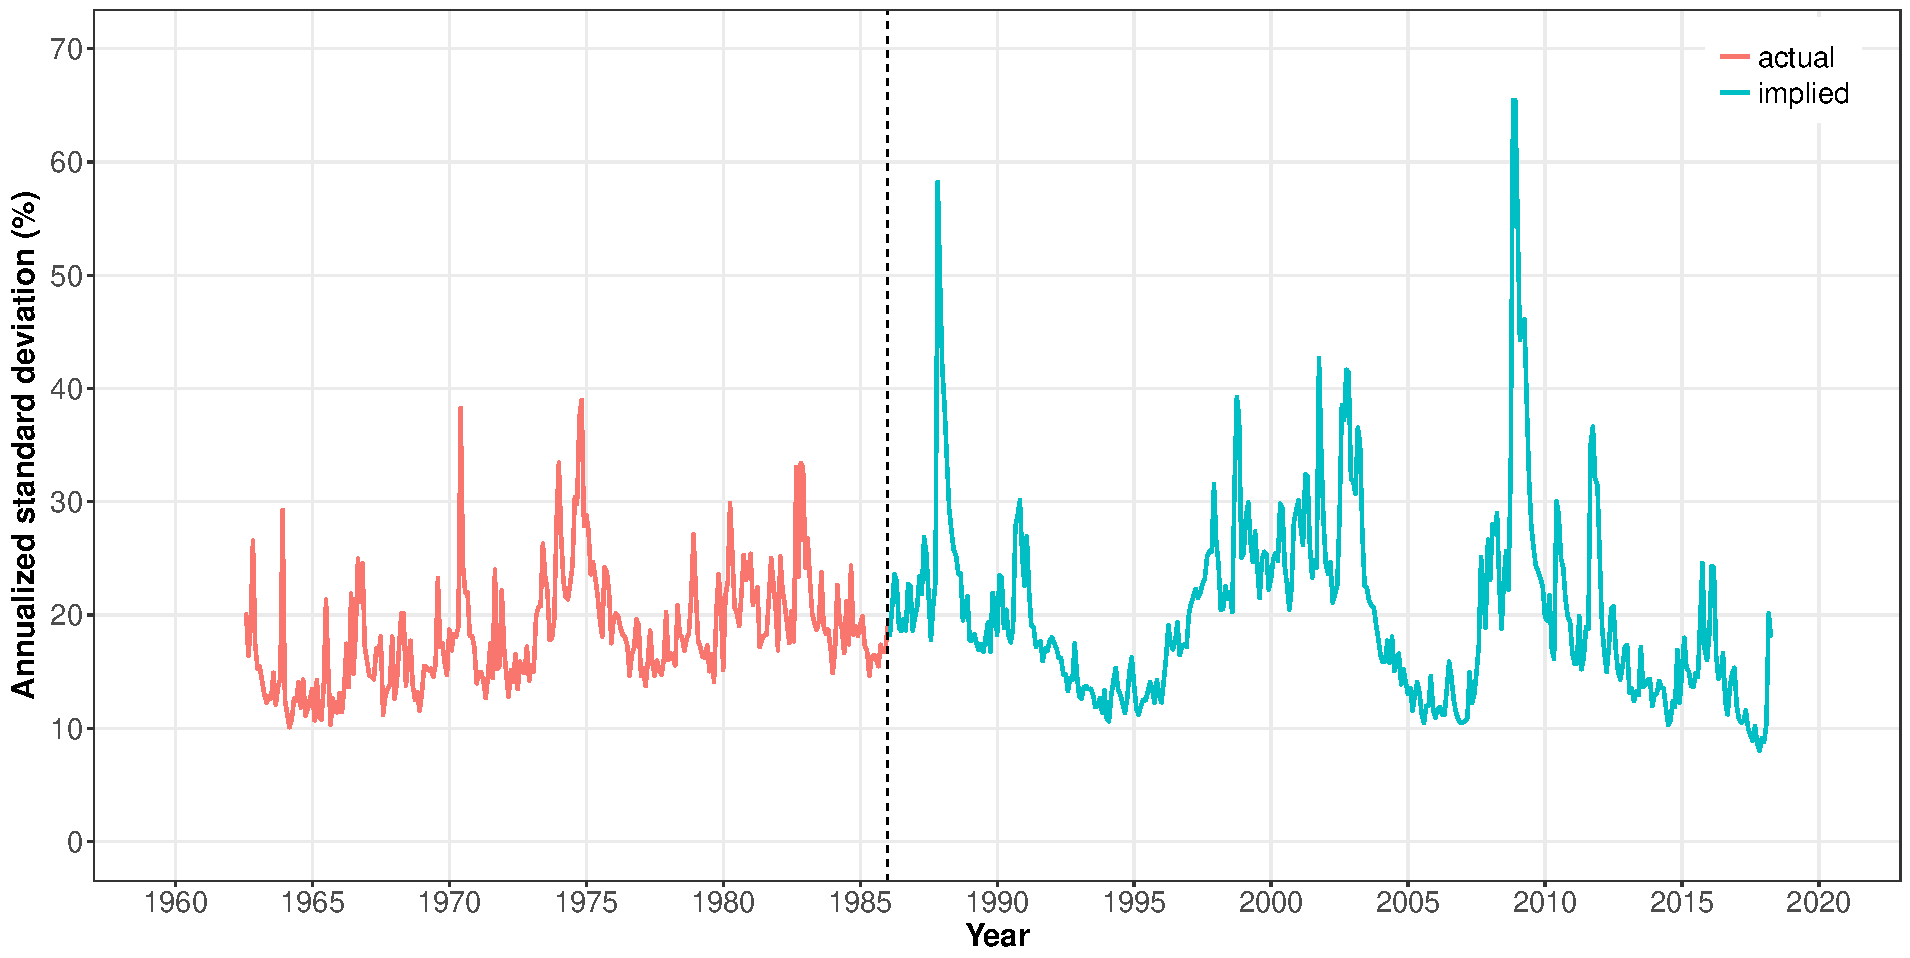
\includegraphics[trim=1cm -1cm 0.8cm 0.5cm, width=0.95\textwidth]{volatility.pdf}}
      \caption[Monthly U.S. stock market volatility including NBER recession dates.]{Monthly U.S. stock market volatility including NBER recession dates (shaded).
      \textit{Note:} From 1986 onwards the series shows the CBOE VXO index of percentage implied volatility, on a hypothetical at the money S\&P100 option 30 days to expiration. Before 1986 actual monthly return volatilities are calculated as the monthly standard deviation of the daily S\&P500 index normalized to the same mean and variance as the VXO index when they overlap from 1986 - 2003.}
   \label{fig:volatility}
\end{figure}

%\begin{figure}[!h]
%   \centering
%   \setlength\fboxsep{0pt}
%   \setlength\fboxrule{0pt}
%   \fbox{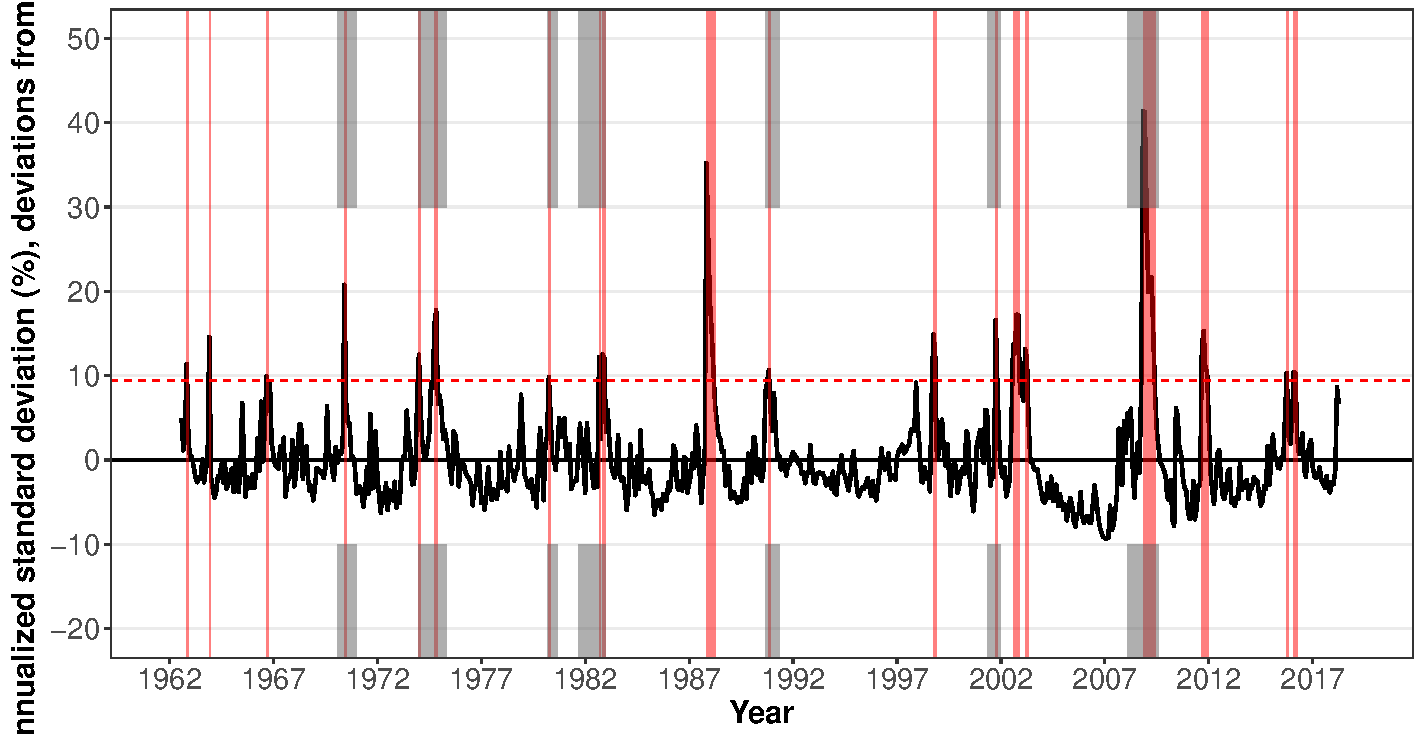
\includegraphics[trim=1cm -2.5cm 0.8cm -1cm, width=0.95\textwidth]{volatility_cycle_shocks2.pdf}}
%      \caption[Monthly U.S. stock market volatility including Bloom-shocks and NBER recession dates.]{Monthly U.S. stock market volatility. Red shaded areas correspond to dates where volatility series exceeds 1.65 standard deviation above the series' mean. Grey shaded areas denote NBER recession dates in the US.}   \label{fig:volatility_cycle_shocks2}
%\end{figure}


%\begin{figure}[hbt]
%   \centering
%   \setlength\fboxsep{0pt}
%   \setlength\fboxrule{0pt}
%   \fbox{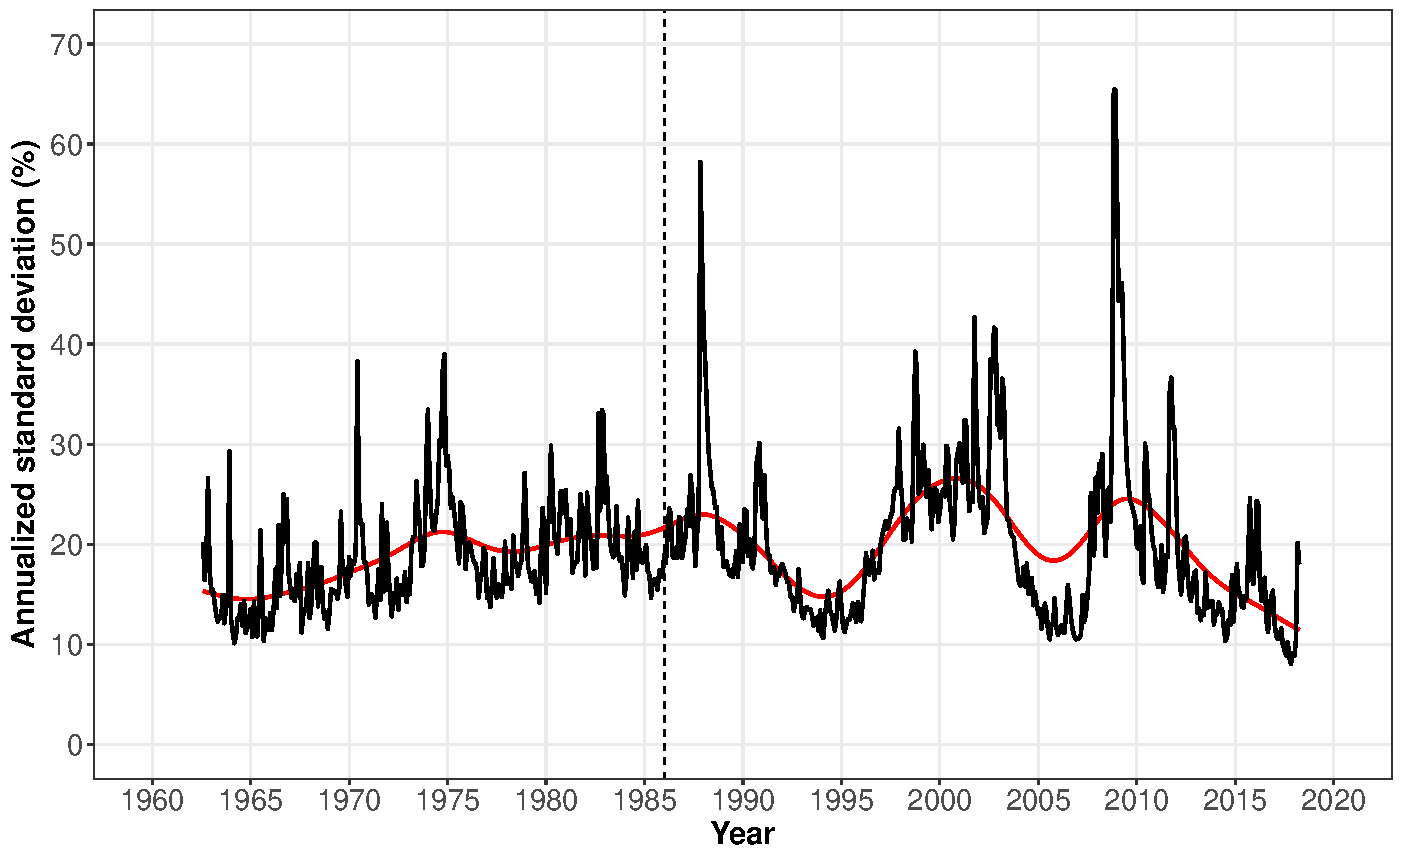
\includegraphics[trim=1cm -2.5cm 0.8cm -1cm, width=0.95\textwidth]{volatility_trend.pdf}}
%      \caption[Monthly U.S. stock market volatility and HP-filtered trend.]{Monthly U.S. stock market volatility and HP-filtered trend.
%      \textit{Note:} HP-filtered trend was calculated using a smoothing parameter $\lambda = 129,6000$.}   \label{fig:volatility_trend}
%\end{figure}


%\begin{figure}[h]
%   \centering
%   \setlength\fboxsep{0pt}
%   \setlength\fboxrule{0pt}
%   \fbox{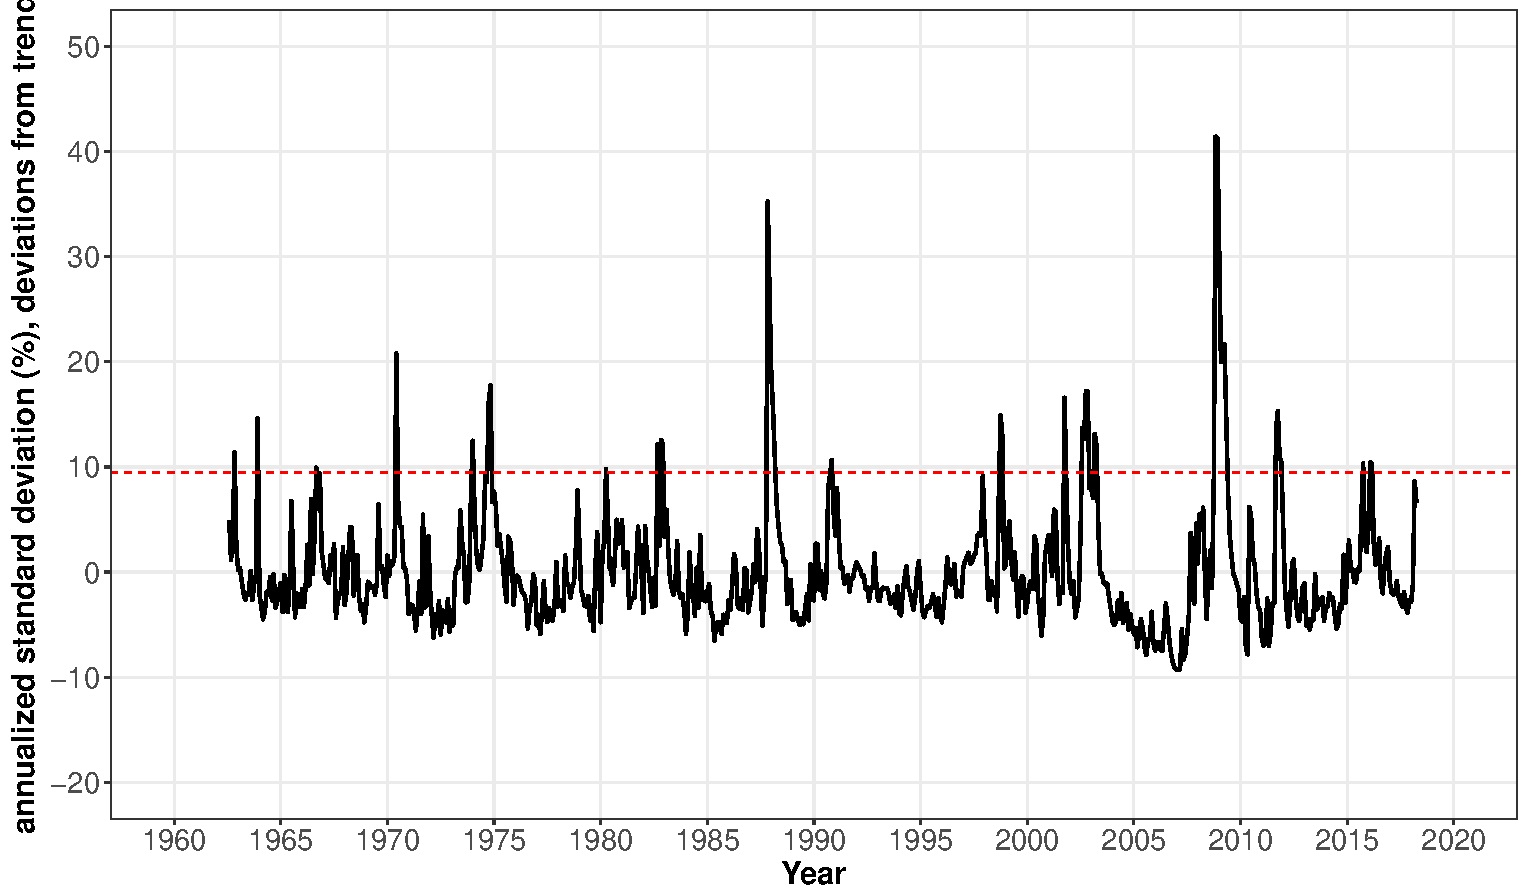
\includegraphics[trim=1cm -2.5cm 0.8cm -1cm, width=0.95\textwidth]{volatility_cycle_shocks.pdf}}
%      \caption[Monthly U.S. stock market volatility and HP-filtered trend.]{Monthly U.S. stock market volatility and HP-filtered trend.
%      \textit{Note:} HP-filtered trend was calculated using a smoothing parameter $\lambda = 129,6000$.}   \label{fig:volatility_cycle_shocks}
%\end{figure}

%
%
%\begin{table}[htp] 
%\centering
%\caption{Replication of shocks following \citet{bloom:09}.}
%\scalebox{0.8}{
%    \begin{tabular}{cccccc}
%    \hline
%         yearmon_start & yearmon_end & duration & yearmon_max & max_vol \\ \hline
%        Nov 1962 & Nov 1962 & 1 months & Nov 1962 & 26.58\% \\
%        Dec 1963 & Dec 1963 & 1 months & Dec 1963 & 29.28\% \\
%        Sep 1966 & Sep 1966 & 1 months & Sep 1966 & 24.99\%\\
%        Jun 1970 & Jun 1970 & 1 months & Jun 1970 & 38.27\% \\
%        Jan 1974 & Jan 1974 & 1 months & Jan 1974 & 33.44\% \\
%        Oct 1974 & Nov 1974 & 1 months & Nov 1974 & 38.98\% \\
%        Apr 1980 & Apr 1980 & 1 months & Apr 1980 & 29.86\% \\
%        Sep 1982 & Sep 1982 & 1 months & Sep 1982 & 33.05\% \\
%        Nov 1982 & Dec 1982 & 2 months & Nov 1982 & 33.43\% \\
%        Nov 1987 & Mar 1988 & 5 months & Nov 1987 & 58.22\% \\
%        Nov 1990 & Nov 1990 & 1 months & Nov 1990 & 30.13\% \\
%        Oct 1998 & Nov 1998 & 1 months & Oct 1998 & 39.25\% \\
%        Oct 2001 & Oct 2001 & 1 months & Oct 2001 & 42.69\% \\
%        Aug 2002 & Nov 2002 & 4 months & Oct 2002 & 41.66\% \\
%        Mar 2003 & Apr 2003 & 1 months & Mar 2003 & 36.54\% \\
%        Nov 2008 & May 2009 & 7 months & Nov 2008 & 65.45\% \\
%        Sep 2011 & Dec 2011 & 4 months & Oct 2011 & 36.64\% \\
%        Oct 2015 & Oct 2015 & 1 months & Oct 2015 & 24.60\% \\
%        Feb 2016 & Mar 2016 & 2 months & Feb 2016 & 24.33\% \\
%        \hline
%        \hline
%    \end{tabular}
%}
%\label{tab:bloom_shocks}
%\end{table}


\subsection{A News-Based Measure: \citet{bakeretal:15}}
\label{sec:epuindex}
While string searching (and hence also matching) algorithms have been around since the early days of computer science, the methods rose in sophistication in the past decades accompanying ever larger amounts of text. Increased computing power in combination with more efficient algorithms nowadays allows the processing of masses of text within a reasonable amount of time. In combination with dedicated digital archives of various sorts, a rapidly growing body of literature within economics has turned to text search methods, primarily using digital newspaper archives, to answer a variety of research questions.\footnote{Examples of such approaches include, among others, \citet{alexopoulosandcohen:09}, \citet{genthkowandshapiro:10}, \citet{hobergandphillips:10}, \citet{boudoukhetal:13}, and \citet{alexopoulosandcohen:15}.}

Making use of this newspaper-based technique and with a focus on \textit{policy-related} economic uncertainty, \citet{bakeretal:15} build uncertainty indices trying to capture both the public's near-term and longer-term concerns as reflected in the newspaper coverage of certain key-terms\footnote{In earlier drafts of their contribution, index components included the present value of future scheduled tax code expirations and disagreement among professional forecasters over future government purchases and consumer prices. To be able to extend their EPU measures over time and across countries, \citet{bakeretal:15} decided to focus on the newspaper approach but continue to report the other components on their dedicated website at \url{http://www.policyuncertainty.com}.}. The cornerstone of their work is the construction of a monthly and daily Economic Policy Uncertainty (EPU) Index for the U.S. and its evolution since 1985. This index reflects the frequency with which a specifically designed trio of terms is found in digital archives containing articles of ten leading U.S. newspapers:\footnote{The newspapers filtered by the search-algorithm are \textit{USA Today}, \textit{Miami Herald}, \textit{Chicago Tribune}, \textit{Washington Post}, \textit{Los Angeles Times}, \textit{Boston Globe}, \textit{San Francisco Chronicle}, \textit{Dallas Morning News}, \textit{New York Times} and \textit{Wal Street Journal}.} ``economic'' or ``economy'' (E-terms set); ``uncertain'' or ``uncertainty'' (U-terms set); and one or more of the terms ``Congress'', ``deficit'', ``Federal Reserve'', ``legislation'', ``regulation'' or ``White House'' (P-terms set). This means that to be of relevance, an article must contain terms in all of the three categories.

\begin{figure}[!h]
   \centering
   \setlength\fboxsep{0pt}
   \setlength\fboxrule{0pt}
   \fbox{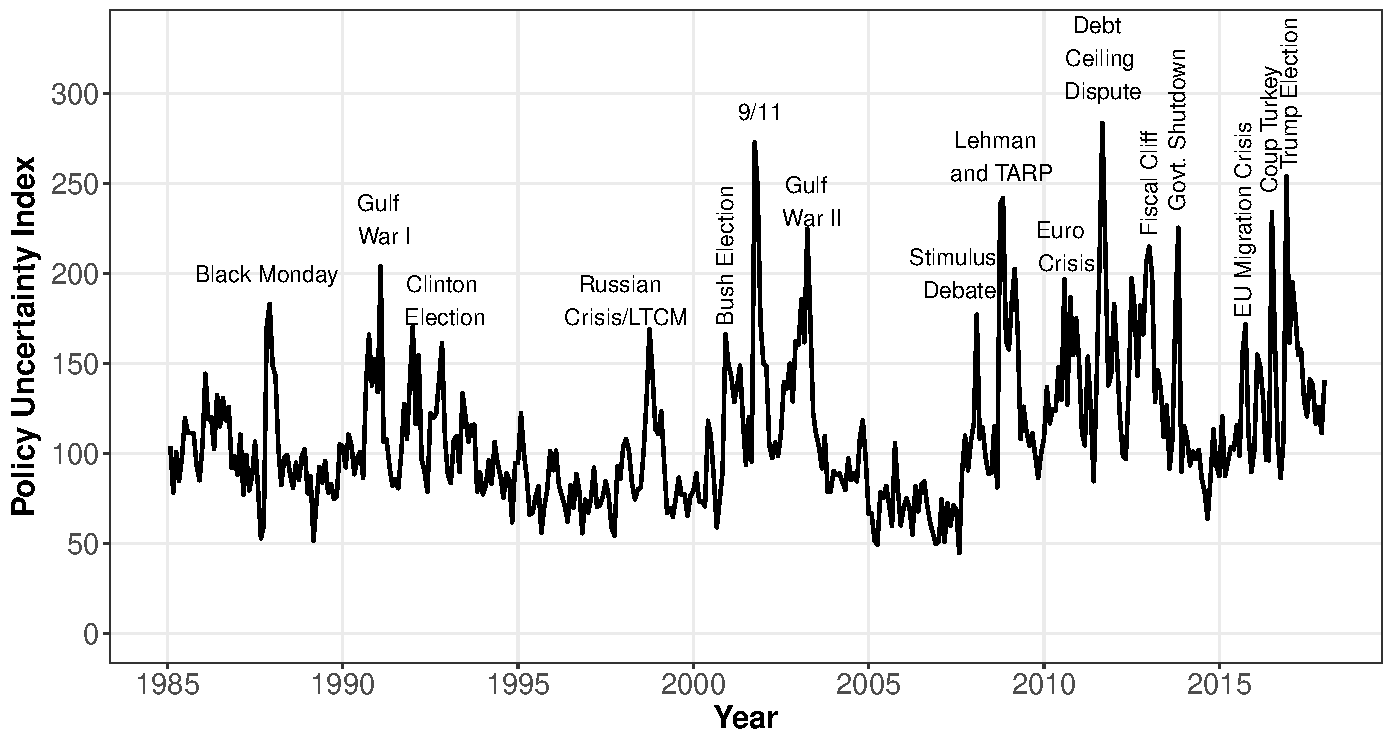
\includegraphics[trim=0.5cm -1.5cm 0.8cm 0cm, width=0.95\textwidth]{epu_index_plot.pdf}}
      \caption[EPU Index for the U.S., 01/1985 - 04/2018.]{EPU Index for the U.S., 01/1985 - 04/2018.
      \textit{Note:} Index reflects scaled monthly counts of articles containing 'uncertain' or 'uncertainty', 'economic' or 'economy, and one or more policy relevant terms: 'regulation', 'federal reserve', 'deficit', 'congress', 'legislation', or 'white house'. The series is normalized to mean 100 from 1985-2009 and based on queries run for the USA Today, Miami Herald, Chicago Tribune, Washington Post, LA Times, Boston Glove, SF Chronicle, Dallas Morning News, NW Times, and the Wall Street Journal. Shaded areas denote NBER recession dates in the U.S.\\
      Original Figure in \citet{bakeretal:15} ranges until 2015. We have taken all available values until April 2018, inclusive.}   \label{fig:epuindex}
\end{figure}

To cater for the discrepancy of the overall volume of articles across newspapers and time yielded by the raw counts, \citet{bakeretal:15} implement the following steps to arrive at a reasonable index: (i) scaling of the raw counts by the total number of articles in the same newspaper and month, (ii) standardization of each monthly newspaper-level series to unit standard deviation from 1985 to 2009, (iii) averaging across the 10 papers by month, (iv) normalization of the 10-paper series to a mean of 100 from 1985 to 2009.

As shown in Figure~\ref{fig:epuindex}, this results in a time series that, among others, spikes near tight presidential elections, Gulf Wars I and II, the 9/11 attacks, the failure of Lehman Brothers, the 2011 debt ceiling dispute, and other major battles over fiscal policy \citep{bakeretal:15}. As an example of a period where the EPU index does not show any outlier, \citet{bakeretal:15} refer to the partial federal government shutdowns from November 1995 to January 1996.\footnote{Although these shutdowns did receive a considerable amount of press coverage, the share of articles mentioning the established trio of terms is extremely low.} 



Besides this index, \citet{bakeretal:15} extend their approach back in time, across countries (by constructing indices for 11 other countries including all G10 economies), and to specific (policy) categories.
 
 \begin{figure}[h]
   \centering
   \setlength\fboxsep{0pt}
   \setlength\fboxrule{0pt}
   \fbox{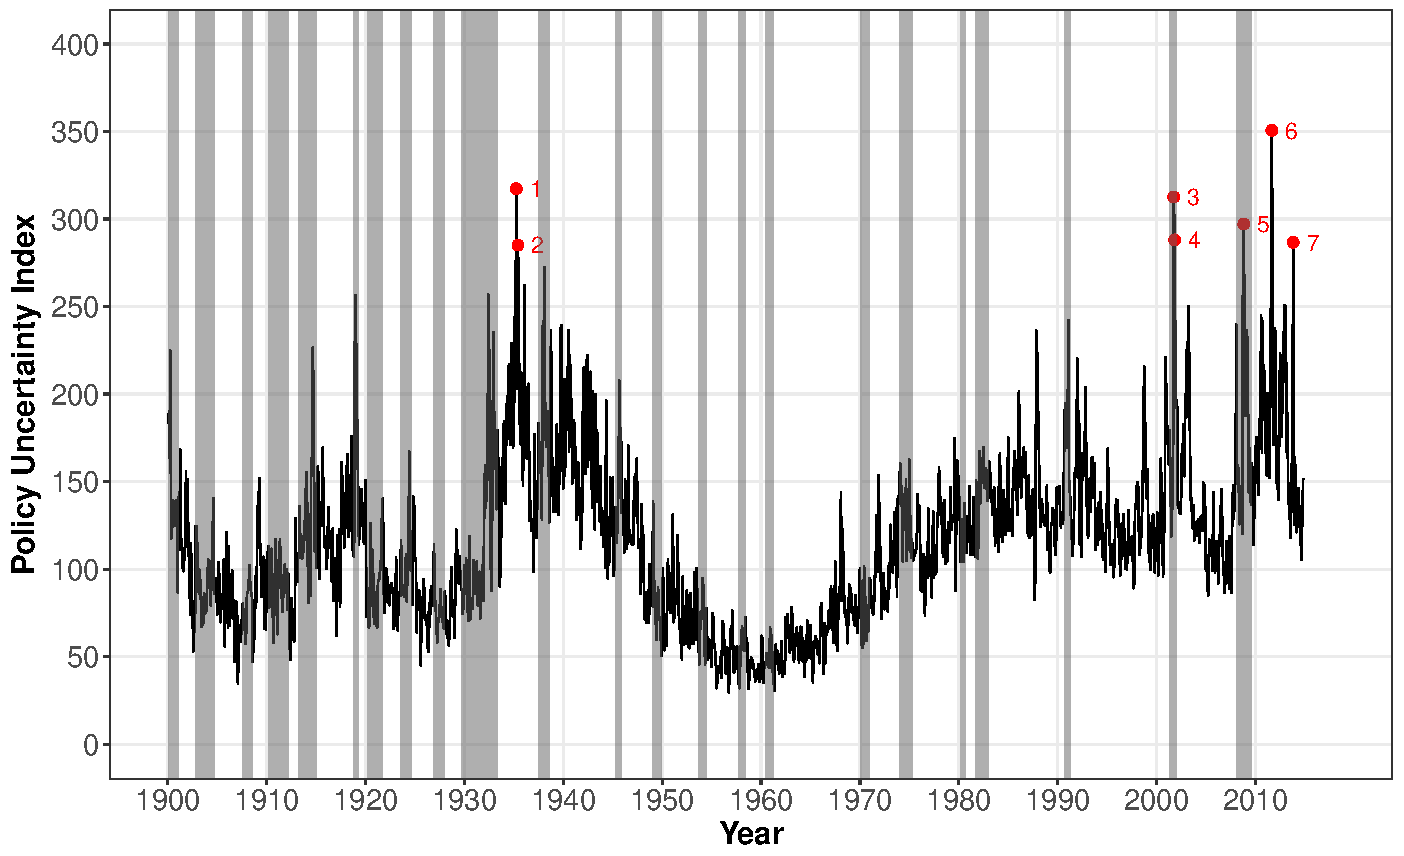
\includegraphics[trim=0.5cm -1.5cm 0.8cm 0cm, width=0.95\textwidth]{epu_index_historical_plot.pdf}}
      \caption[Historical EPU Index for the U.S., 01/1900 - 10/2014.]{EPU Index for the U.S. , 01/1900 - 10/2014.
      \textit{Note:} Index reflects scaled monthly counts of articles containing 'uncertain' or 'uncertainty', 'economic' or 'economy, and one or more policy relevant terms: 'regulation', 'federal reserve', 'deficit', 'congress', 'legislation', or 'white house'. The series is normalized to mean 100 from 1985-2009 and based on queries run for the USA Today, Miami Herald, Chicago Tribune, Washington Post, LA Times, Boston Glove, SF Chronicle, Dallas Morning News, NY Times, and the Wall Street Journal. Shaded areas denote NBER recession dates in the U.S.}   \label{fig:epuindex_historical}
\end{figure}
 
For their historical EPU Index dating back to 1900, \citet{bakeretal:15} rely on the archives of six major U.S. newspapers\footnote{They are \textit{Wall Street Journal}, \textit{New York Times}, \textit{Los Angeles Times}, \textit{Boston Globe}, \textit{Chicago Tribune} and \textit{Washington Post}.} that have been published throughout the 20th century with slight modifications: to account for word usage patterns in newspapers, the E term set is expanded to include ``business'', ``industry'', ``commerce'' and ``commercial'' while the P term set is expanded by the words ``tariff'' and ``war''.\footnote{\citet{bakeretal:15} report that for the overlapping period as of 1985 both the original term sets and the expanded ones show similar results while the expanded term set performs better for the first decades of the 20th century.} As shown in Figure~\ref{fig:epuindex_historical}, looking at the index from 1900 onwards, for \citet[p. 1594]{bakeretal:15} the series ``[...] highlights pre-World WAR II political developments and shocks like the Gold Standard Act of 1900, the outbreak of World War I, the Versailles conference in 1919, and a sustained surge in policy uncertainty from late 1931 when President Herbert Hoover, and then President Franklin Roosevelt, introduced a rash of major new policies. [...]'' Interestingly, the index also shows a slight upward drift since the 1960s which \citet{bakeretal:14} attribute either to the growth in government spending, taxes, and regulation or increased political polarization and its implications for the policy-making process. Corresponding to Figure~\ref{fig:epuindex_historical}, Table~\ref{tab:largest_epu} showing the dates marked with red dots reveals that in the past two decades five times uncertainty rose to levels comparable to the Great Depression of the 1930s.




\begin{table}[!h]
\centering
\caption{7 Largest Spikes of U.S. EPU Historical}
\scalebox{1}{ 
    \begin{tabular}{cccc}
        \hline
         ID & Year & Month & EPU Historical Index \\ \hline
        1 & 1935 & 3 & 317 \\
        2 & 1935 & 5 & 285 \\
        3 & 2001 & 9 & 313 \\
        4 & 2001 & 10 & 288 \\
        5 & 2008 & 10 & 297 \\
        6 & 2011 & 8 & 351 \\
        7 & 2013 & 10 & 287 \\
            \hline
                \hline
    \end{tabular}
}
\label{tab:largest_epu}
\centering
\end{table}

The category-specific policy uncertainty indices are developed for the U.S. only by specifying more restrictive criteria for those articles that contain certain search terms.\footnote{E.g., the construction of a health care policy- or national security policy uncertainty index is based on the presence of additional terms like ``health care'', ``hospital'' or``health insurance'' and ``war'', ``terrorism'' or ``department of defense'', respectively.}\footnote{Together, the collection of all indices is available at \url{http://www.policyuncertainty.com}, a dedicated homepage by the authors to make regular updates to their indices available.}

Table~\ref{fig:epuindex_categories} reports all category-specific EPU indices together with an overall economic uncertainty (EU) index (dropping the third of the trio of necessary terms in the index constructions) and the EPU. --> Refer to \citet[p. 1602]{bakeretal:15} to add some details about the peculiarities of the categorical breakdown of EPU!


 \begin{figure}[!h]
   \centering
   \setlength\fboxsep{0pt}
   \setlength\fboxrule{0pt}
   \fbox{\includegraphics[trim=0.5cm -1.5cm 0.8cm 0cm, height=5cm, width=12cm]{example-image-b}}
      \caption[Placeholder for 'Economic Policy Uncertainty by Policy Category and Time Period, 1985 - 2014.]{Placeholder for 'Economic Policy Uncertainty by Policy Category and Time Period, 1985 - 2014.
      \textit{Note:} The second row reports average values of the Newsbank Index of Economic Policy Uncertainty in each indicated period (scaling by the total number of articles in a period), expressed as a percentage of the average index value for the entire sample period from 1985:1 to 2014:12. For example, the value of 109 for Economic Policy Uncertainty from 1985:1 to 1990:6 says that the value of the index in that period is 109\% of its average value over the full sample period. The top row reports the value of the Newsbank Index of Overall Economic Uncertainty, also expressed as a percentage of the average value of the news-based policy uncertainty index. Entries in Rows 1 to 12 index report analogous values for narrower policy categories based on news article references to specific policy-related terms. For example, the value of 26.8 for “Monetary Policy” from 2010:1 to 2013:10 says that the number of scaled references to monetary policy uncertainty in this period is 26.8 percent of the
average number of scaled references to ALL forms of policy-related uncertainty during the 1985:1 to 2012:10 sample period. The categories in Rows 1 through 12 are not mutually exclusive in two respects. First, a given news article may discuss multiple distinct sources of uncertainty such as monetary policy and entitlement reforms. Second, some of the category boundaries overlap. For example, Medicaid is an entitlement program and a major part of the U.S. health care system. \textit{Source: http://www.policyuncertainty.com}}   \label{fig:epuindex_categories}
\end{figure}



To alleviate any potential concerns about the reliability, accuracy or consistency of their newspaper-based approach, \citet[p. 1595]{bakeretal:15} counter with five observations that, in their view, reinforces their indices' ultimate purpose to proxy for movements in policy-related economic uncertainty: (1) there is a strong positive relationship between their EPU measure and implied stock market volatility (as another commonly used uncertainty-proxy)\footnote{We report our correlation-measures in Table~\ref{tab:correlations}.}, (2) they report a strong positive relationship between the newspaper-based EPU index and e.g., indices based on the frequency with which the Federal Reserve System's Beige Books mention policy uncertainty, (3) there seems to be no political slant since EPU indices based on right- or left-wing newspapers show not serious distortions, (4) an extensive audit study that included the manual reading of 12,000 randomly selected articles drawn from major U.S. newspapers which revealed a high correlation between this human- and the classical computer-generated index confirming the chosen set of terms used for the automated text search and lastly, (5) the market adoption of their indices by commercial data providers including Bloomberg, FRED, Haver, and Reuters to alleviate the demands from industry leads \citet{bakeretal:15} to conclude that the indices contain useful information for decision makers.



\begingroup
    \fontsize{8pt}{12pt}\selectfont
    Note to self:
\begin{itemize}
	\item  BBD-index following \citet{bakeretal:15}\\
The IMF Working Paper (Measuring Global and Country-Specific Uncertainty) is a very helpful resource because: (1) They compare various uncertainty measures and also give a hint of from where to retrieve news-based uncertainty-measures!
	\item \citet[p. 1593]{bakeretal:15} write: ``At the macro level, innovations in policy uncertainty foreshadow declines in investment, output, and employment in the United States and, in a panel vector autoregressive setting, for 12 major economies.''
	\item \citet[p. 1596]{bakeretal:15} write: ``Our second approach fits vector autoregressive (VAR) models to U.S. data [...]. The U.S. VAR results indicate that a policy uncertainty innovation equivalent to the actual EPU increase from 2005-2006 to 2001-2012 foreshadows declines of about 6\% in gross investment, 1.1\% in industrial production, and 0.35\% in employment.
\end{itemize}
\endgroup






\subsection{A Forecast-Based Measure: \citet{juradoetal:15}}
\label{sec:macrouncertainty}
\begingroup
    \fontsize{8pt}{12pt}\selectfont
    Note to self:
\begin{itemize}
	\item  \citet[p. 1]{gilchristetal:14} write: ``[...] the common variation in the unforecastable component of a large number of economic indicators \citep{juradoetal:15}.''
\end{itemize}
\endgroup

Especially in contrast to stock market volatility and/or cross-sectional dispersion measures frequently deployed in uncertainty studies, \citet{juradoetal:15} have designed a computationally and data-intensive approach by making use of a rich set of time series, computing the conditional volatility of the unforecastable component of the future value of each of these series and finally aggregating these conditional volatilities into one composite index.\footnote{Note that, apart from practical issues, \citet[p. 1191]{juradoetal:15} themselves explain the reliance on (most likely revised) ``historical'' data (instead of ``real time'' data) with their goal of forming the ``[...] most historically accurate estimates of uncertainty at any given point in time in [their] sample''.}\\
\\
To set their approach apart from other commonly used uncertainty measures, \citet[p. 1178]{juradoetal:15} argue that ``[...] what matters for economic decision making is not whether particular economic indicators have become more or less variable or disperse \textit{per se}, but rather whether the economy has become more or less \textit{predictable}; that is, less ore more uncertain.''\\
\\
To formalize the rationale behind their approach, they define the $h$-period ahead uncertainty in the variable $y_{jt} \in Y_t = (y_{1t}, \ldots, y_{N_{y}t})'$, denoted by $U^t_{jt}(h)$, as the conditional volatility of the purely unforecastable component of the future value of the series, i.e.,
\begin{equation} \label{eq:juradoetal_1}
U^t_{jt}(h) \equiv \sqrt{\mathbb{E}\Big[(y_{jt+h} - \mathbb{E}[y_{jt+h}|I_t])^2|I_t\Big]},
\end{equation}
where the expectation $\mathbb{E}(\cdot|I_t)$ is taken with respect to information $I_t$ available to economic agents at time $t$. Hence, if the expectation today (conditional on all available information) of the squared error in forecasting $y_{jt+h}$ rises, uncertainty in the variable increases. The individual uncertainties at each date are then aggregated into a \textit{macroeconomic uncertainty} index by using aggregation weights $w_j$ as follows:
\begin{equation} \label{eq:juradoetal_2}
U^t_{jt}(h) \equiv plim_{N_{y}\to\infty} \sum_{j=1}^{N_y} w_j U_{jt}^y(h) \equiv \mathbb{E}_w \Big[U_{jt}^y(h)\Big]
\end{equation}

Based on the above definitions, \citet{juradoetal:15} emphasize two features that are central to their approach:
\begin{enumerate}
	\item they distinguish between \textit{uncertainty} in a series $y_{jt}$ and its \textit{conditional volatility} and argue that the proper measurement of uncertainty requires the removal of the entire forecastable component $\mathbb{E}[y_{jt+h}|I_t]$ before the computation of the conditional volatility; without accounting for this, the argument goes, forecastable variation is erroneously classified as ``uncertainty''. According to \citet{juradoetal:15}, this is taken into account only in very few occasions in the literature.
	\item they claim that macroeconomic uncertainty is ``a measure of the common variation in uncertainty across many series'' and not equal to the uncertainty in any single series $y_{jt}$; \citet{juradoetal:15} see this as an important argument because of uncertainty-based theories of the business cycle that typically require the existence of common (often countercyclical) variation in uncertainty across large numbers of series; \citet{juradoetal:15} hence put their econometric estimation of uncertainty insofar to test, as they expect to find evidence of such an aggregate uncertainty factor common to many series, if the above assumption turns out to be correct.
\end{enumerate}

\citet{juradoetal:15}'s econometric approach then consists of three parts:
\begin{enumerate}[i]
	\item estimation of the forecastable component $\mathbb{E}[y_{jt+h}|I_t]$: this is achieved by, first, running a factor analysis on a large set of predictors (132 macro time series) $\{X_{it}\}, i = 1, 2, \dots, N$ whose linear span/hull comes as close as possible to $I_t$; second, making use of the formed factors, $\mathbb{E}[y_{jt+h}|I_t]$ is then approximated by means of a diffusion index forecasting model ideal for data-rich environments (the diffusion indices can then be treated as known in the subsequent steps)
	\item with the definition of the $h$-step-ahead forecast error as $V_{jt+h}^y \equiv y_{jt+h} - \mathbb{E}[y_{jt+h}|I_t]$, \citet{juradoetal:15} estimate the conditional volatility of this forecast error, i.e., $\mathbb{E}[(V_{t+h}^y)^2|I_t]$ at time $t$ by specifying a parametric stochastic volatility model for both the one-step-ahead prediction errors in $y_{jt}$ and the analogous forecast errors for the factors (from step i above); \\
	these volatility estimates are then used to recursively compute the values of $\mathbb{E}[(V_{t+h}^y|I_t]$ for $h > 1$. 
	\item in the last step, the \textit{macroeconomic uncertainty} index $U_t^y(h)$ is constructed from the individual uncertainty measures $U_{jt}^y(h)$ where the base-case is the equally-weighted average of individual uncertainties
\end{enumerate}

While \citet{juradoetal:15} apply their approach to two large dataset with economic time-series (one monthly dataset containing hundreds of macroeconomic and financial indicators and one quarterly dataset containing 155 firm-level observations on profit growth normalized by sales), here we only confine ourselves to the former, i.e., their \textit{common macro uncertainty} index.

Their resulting estimated measures of time-varying uncertainty are plotted in Figure~\ref{fig:macroUncertainty_index} and reveals 'only' three big episodes of uncertainty: the months during the recessions from 1973-1974 and 1981-1982 and the months during the Great Recession of 2007-2009 (being the most striking episode of heightened uncertainty, followed by the 1981-1982 recession as a close second).\footnote{See Table~\ref{tab:macro_shocks} below for the exact dates including the maximum value for the index for each identified episode of high uncertainty.}\footnote{\citet{juradoetal:15} report that a closer look at the estimates reveals that the three series with the highest uncertainty are a producer price index for intermediate materials, a commodity spot price index, and employment in mining between 1973:11 and 1975:3, the Fed funds rate, employment in mining, and the three months commercial paper rate for the 1980:1 and 1982:11 episode and the monetary base, non-borrowed reserves and total reserves between 2007:12 and 2009:6. \citet{juradoetal:15} conclude these results to be consistent with the historical account.}

\begin{figure}[!ht]
   \centering
   \setlength\fboxsep{0pt}
   \setlength\fboxrule{0pt}
   \fbox{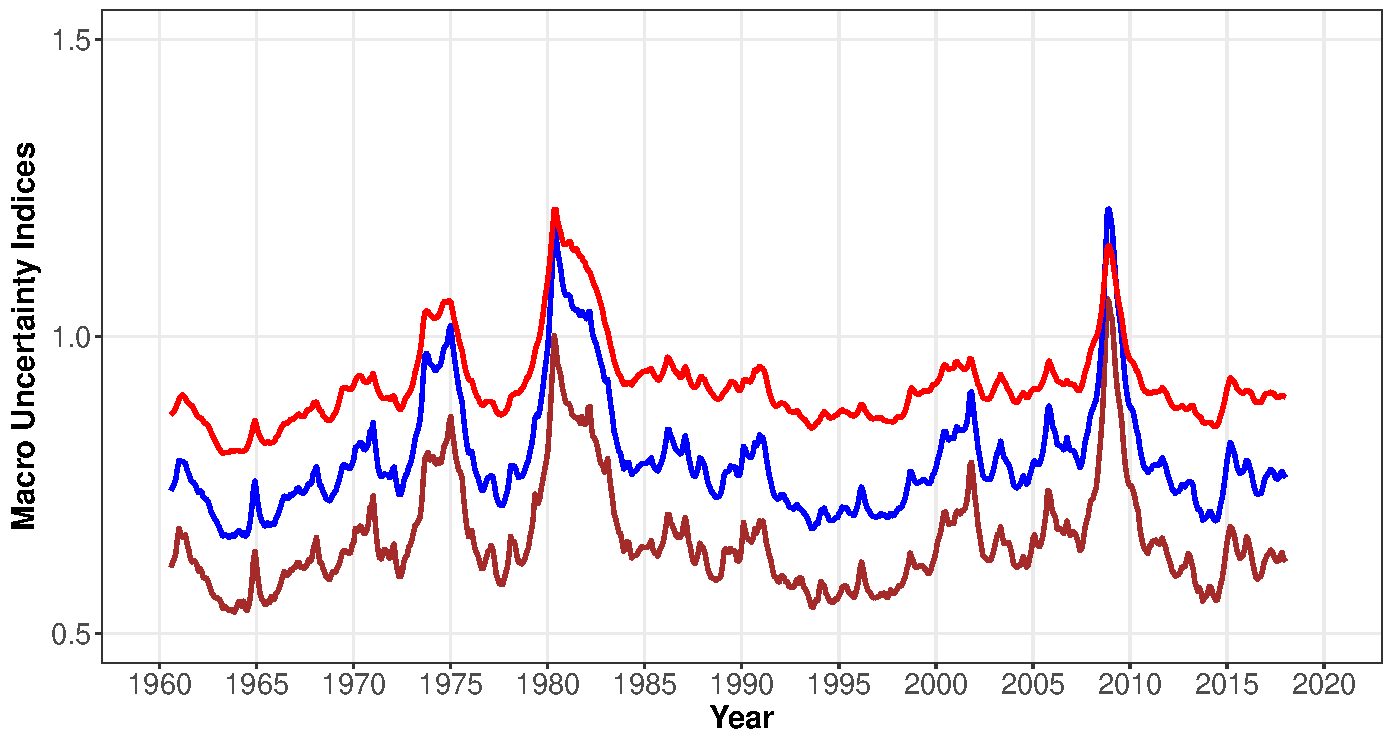
\includegraphics[trim=0cm -2cm 0cm -0.5cm, clip, height=0.6\textwidth, width=1\textwidth]{macroUncertainty_index_plot.pdf}}
      \caption[Aggregate Uncertainty: $h = 1, 3, 12$.]{Aggregate Uncertainty: $h = 1, 3, 12$.
      \textit{Note:} Horizontal lines indicate 1.65 standard deviations above the mean of each series. Data are monthly and span the period 1960:7-2017:12. Red shaded areas correspond to dates where volatility series exceeds 1.65 standard deviation above the mean of the h1-series. Grey shaded areas denote NBER recession dates in the US.\\
      Original Figure 1 in \citet{juradoetal:15} spans until 2011. We have taken all available values until December 2017, inclusive.}   \label{fig:macroUncertainty_index}
\end{figure}

\begin{table}[t]
\centering
\caption{Periods of high uncertainty according to macro uncertainty index h=1.}
\scalebox{0.8}{
    \begin{tabular}{ccccc}
    \hline
         Start & End & Duration & Maximum Year/Month & Maximum Value \\ \hline
        Sep 1974 & Mar 1975 & 7 months & Jan 1975 & 0.87 \\
        Jan 1980 & Aug 1982 & 31 months & May 1980 & 1.00 \\
        Jul 2008 & Sep 2009 & 15 months & Nov 2008 & 1.06 \\
        \hline
        \hline
    \end{tabular}
}
\label{tab:macro_shocks}
\centering
\end{table}


The IMF Working Paper (Measuring Global and Country-Specific Uncertainty) is a very helpful resource because: (4) They also succinctly describe the uncertainty-measure developed by Jurado et al (which is very complicated!)




%\subsection{Additional Parts for Later Usage}
%\citet{orlikandveldkamp:14} discuss data used to proxy for uncertainty in Section 5 and offer a useful taxonomy which we could make use of as well! They write: ``Our model generates a measure of economic uncertainty. In this section, we describe the commonly used proxies of uncertainty, analyze their theoretical relationship with conditional variance and then compare their statical properties to those of our measure. \citet{orlikandveldkamp:14} mention the following uncertainty measures:\\
%\\
%\\
%\\
%\\
%Another interesting sentence that is written in \citet{bachmannetal:13}, p. 10: ``Measuring the subjective uncertainty of decision makers is inherently difficult. Ideally, one would like to elicit a subjective probability distribution over future events from the managers, as has been done in Guiso and Parigi (1999) for Italian firms. with this probability distribution it is straightforward to compute a measure of subjective uncertainty for firms' decision makers. However, to the best of our knowledge such probability distributions are not available repeatedly and over long time horizons. Therefore, reserachers have to rely on proxies.'' \\
%\\
%\\
%\\
%Note to self: 
%\begin{itemize}
%	\item I could potentially at some point refer to economic sentiment indicators like \url{https://www.oenb.at/en/Statistics/Standardized-Tables/
%	Economic-and-Industry-Indicators/Economic-Indicators/Economic-Sentiment-Indicator-for-the-Euro-Area.html} or \url{https://data.europa.eu/euodp/data/dataset/c04BuUz6WXIQGJkHPwLug}
%\end{itemize}

\subsection{Critique of the Various Measures}
\begin{itemize}
	\item Comparing the VXO to their own macro uncertainty index, \citet[p. 1201]{juradoetal:15} write that ``[...] it is difficult to imagine that the level of macro uncertainty in the economy in October 1987 (not even a recession year) was on par with the recent financial crisis.''
	\item \citet{orlikandveldkamp:14} go on and write: ``Other proxy variables for uncertainty are informative, but have a less clear connection to a conditional variance definition of uncertainty.' (then they go on and write about business or consumer confidence, market volatility index (VIX), etc.)'
	\item mentioned in \citet[p. 1182]{juradoetal:15}: ``[...] we emphasize here that the measures of dispersion and stock market volatility studied may or may not be tightly linked to true economic uncertainty. Indeed, one of the most popular proxies for uncertainty is closely related to financial market volatility as measured by the VIX, which has a large component that appears driven by factors associated with time-varying risk-aversion rather than economic uncertainty (see \citet{bekaertetal:13}) 
	\item \citet[p. 4]{moore:17} writes: ``The drawback of these stock volatility measures is that they are only indirectly connected to economic activity. Although company earnings are connected to economic activity, much of the short-run variation in stock prices is driven by other factors (Shiller 1981; Cochran e2011). Although these factors may related to economic uncertainty, the connection to economic activity is not clear. These measures are also asymmetric - increases in the measures accompany large falls in stock prices; large gains in stock prices are less common.
	\item IMF Working Paper, Measuring Global and Country-Specific Uncertainty, p.1: ``A ubiquitous proxy is the implied or relaized volatility in stock markets, such as VIX, e.g. Bloom (2009). However, the volatility in Wall Street might not reflect uncertainty in Main Street. For instance, changes in the VIX might be due to leverage or financiel stress, despite low levels of economic uncertainty; For instance, changes in the VIX might be due to leverage or financial stress, despite low levels of economic uncertainty; see Bekaert et al. (2013).
	\item IMF Working Paper, Measuring Global and Country-Specific Uncertainty, p.1: ``\citet{juradoetal:15} develop an alternative measure of economic uncertainty: the common variation in uncertainty across hundreds of economic series. Their measure reflects uncertainty around objective statistical forecasts, rather than perceived uncertainty by market participants. Moreover, as they focus on common, not idiosyncratic, unceratinty, there is no role for private information and heterogeneous agent models.
	\item IMF Working Paper, Measuring Global and Country-Specific Uncertainty, p.1: ``But, like all measurements of this type, this news-based uncertainty measure puts a high bar for the attentiveness of reporters and editors, who might miss uncertainty events if they neglect to write a story on the subject.'' 
	\item IMF Working Paper, Measuring Global and Country-Specific Uncertainty, p.4: Regarding cross-sectional dispersion measures: When disagreement is taken to indicate uncertainty, the underlying assumption is that this inter-personal dispersion measure is an acceptable proxy for the average dispersion of intra-personal uncertainty. As shown by Lahiri and Sheng (2010), however, disagreement is only a part of uncertainty and misses an important component: the volatility of aggregate shocks.
		\item similarly, \citet[p. 12]{bontempietal:16} write: ``The (i) VIX is used in many empirical studies (most prominently in \citet{bloom:09}). But one caveat that emerges from the use of the VIX to proxy uncertainty concerns its ability to represent macroeconomic uncertainty, since it is based on stock market information alone. According to \citet{bekaertetal:13}, the VIX does not only reflect uncertainty but can be broken down into uncertainty and risk-aversion. Since risk aversion accounts for a sizeable part of the VIX,\footnote{For this reason, the VIX is usually referred to as the ``fear index'' (see, e.g., \citet{whaley:00}).}, even more caution should be taken when considering it as a proxy of macro-economic uncertainty.
	\item in their non-technical summary, \citet{bekaertetal:13} write: ``Second, Bloom (2009) and Bloom, Floetotto and Jaimovich (2009) show that heightened
“economic uncertainty” decreases employment and output. It is therefore conceivable that the
monetary authority responds to uncertainty shocks, in order to affect economic outcomes.
However, the VIX index, used by Bloom (2009) to measure uncertainty, can be decomposed
into a component that reflects actual expected stock market volatility (uncertainty) and a
residual, the so-called variance premium, that reflects risk aversion and other non-linear pricing
effects, perhaps even Knightian uncertainty. Establishing which component drives the strong
co-movements between the monetary policy stance and the VIX is therefore particularly
important''
	\item related to our empirical analysis: \citet[p. 1184]{juradoetal:15} write: ``An important unresolved issue for empirical analysis of uncertainty concerns the persistence of uncertainty shocks. [...] Researchers (e.g., Schaal 2011) have argued that empirical proxies for uncertainty, such as the cross-sectional dispersion in firms' sales growth, are not persistent enough to explain the prolonged levels of unemployment that have occurred during and after some recessions, notably the 2007-2009 reession and its aftermath. Here we provide new measures of uncertainty and its persistence, finding that they are considerably more persistent than popular proxies such as stock market volatility and measures of dispersion.
	\item With regard to cross-sectional dispersion measures in $N_A$ analysts' or forms' subjective expectations as a measure of uncertainty, \citet[p. 1182]{juradoetal:15} also have a very strong opinion: ``A separate strand of the literature focuses on cross-sectional dispersion in $N_A$ analysts' or firms' subjective expectations as a measure of uncertainty:
	\begin{equation}\label{eq:juradoetal_3}
D^A_{jt}(h)  = \sqrt{\sum_{k=1}^{N_{A_t}} w_k^A \Big(y_{jt+h} - \mathbb{E} (y_{jt+h}|I_{{A_k}, t})\Big)^2},
	\end{equation}
	where $I_{{A_k}, t}$ is the information of agent $k$ at time $t$, and $w_k^A$ is the weight applied to agent $k$. One potential advantage of using $D^A_{jt}(h)$ as a proxy for uncertainty is that is treats the conditional forecast of $y_{jt+h}$ as an observable variable, and therefore does not require an estimation of $\mathbb{E} (y_{jt+h}|I_{{A_k}, t})$. \citet{bachmannetal:13} follow this approach using a survey of German firms and argue that uncertainty appears to be more an outcome of recessions than a cause, contrary to the predictions of theoretical models such as \citet{bloom:09} and others. [...] While analysts' forecasts are interesting in their own right, there are several known drawbacks in using them to measure uncertainty. First, subjective expectations are only available for a limited number of series. For example, of the 132 monthly macroeconomic series we will consider in this paper, not even one-fifth have corresponding expectations series. Second, it si not clear that the responses elicited from these surveys accurately capture the conditional expectations of the economy as a whole. The respondents typically sampled are practitioner forecasters; some analysts' forecasts are known to display systematic biases and omit relevant forecasting information (So, 2013), and analysts may have pecuniary incentives to bias their forecasts in a way that economic agents would not. Third, disagreement in survey forecasts could be more reflective of differences in opinion than of uncertainty. Fourth, Lahiri and Shen (2010) show that, even if forecasters are unbiased, disagreement in analysts' point forecasts does not equal (average across analysts) forecast error uncertainty unless the variance of accumulated aggregate shocks over the forecast horizon is zero. \citet{bachmannetal:13} acknowledge these problems and are careful to address them by using additional proxies for uncertainty, such as an ex post measure of forecast error variance based on the survey expectations. \\
	
	
	
	\item Further, \citet{juradoetal:15} (pp. 1178) argue, that ``unfortunately, the conditions under which common proxies are likely to be tightly linked to the typical theoretical notion of uncertainty may be quite special. For example, stock market volatility can change over time even if there is no change in uncertainty about economic fundamentals, if leverage changes, or if movements in risk aversion or sentiment are important drivers of asset market fluctuations.\\
Cross-sectional dispersion in individual stock returns can fluctuate without any change in uncertainty if there is heterogeneity in the loadings on common risk factors. similarly, cross-sectional dispersion in firm-level profits, sales, and productivity can fluctuate over the business cycle merely because there is heterogeneity in the cyclicality of firms' business activity.'' 
	\item \citet[p. 13]{bontempietal:16} write: ``Although independent of any single observable economic indicator or event, the macroeconomic uncertainty measure following \citet{juradoetal:15} is a computationally intensive black box that is not directly linked to the uncertainty perceived by the general public.  
\end{itemize}

\section{Properties of Selected Measures and Stylized Facts}
\label{sec:ComparisonOfMeasures}
\begin{figure}[!ht]
   \centering
   \setlength\fboxsep{0pt}
   \setlength\fboxrule{0pt}
   \fbox{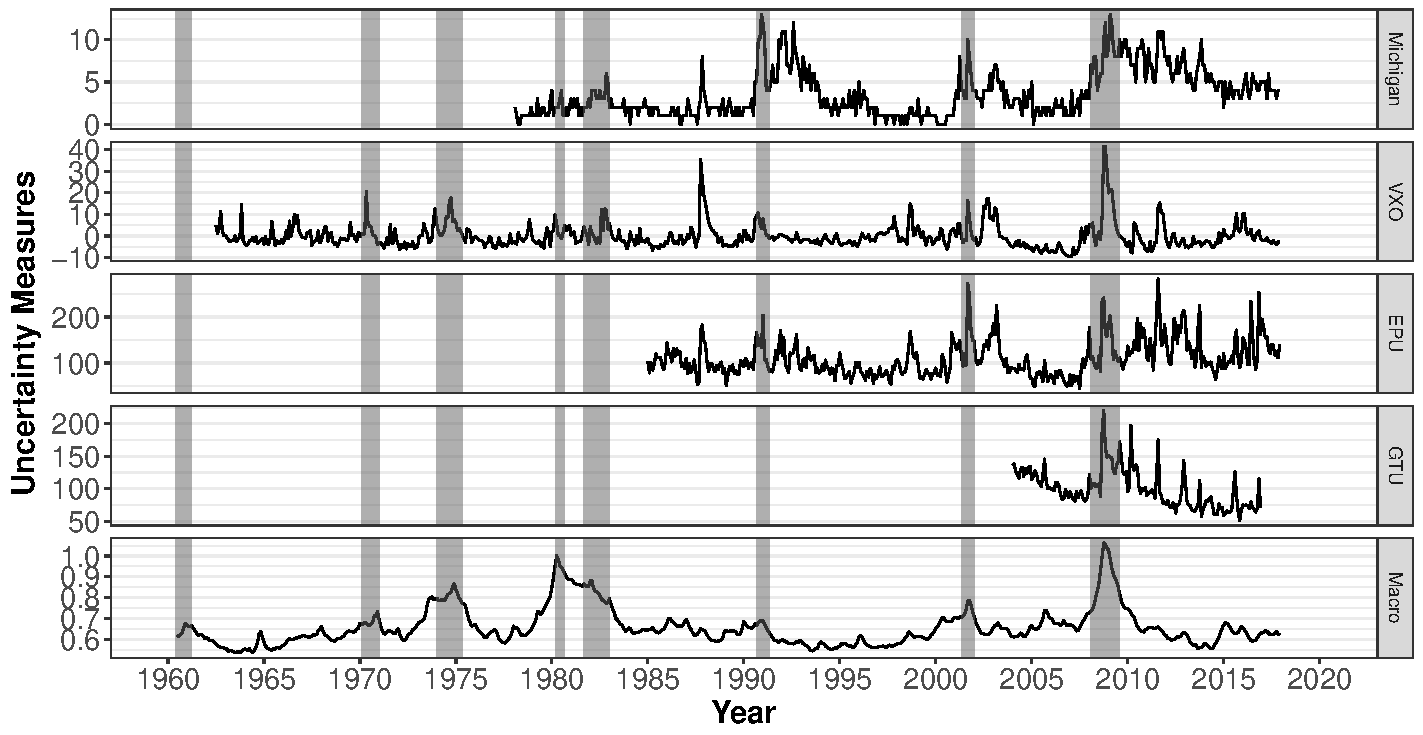
\includegraphics[trim=1cm -1.5cm 0.8cm -0cm, width=0.95\textwidth]{comparison_plot.pdf}}
      \caption[Comparison of uncertainty measures (facetted).]{Comparison of uncertainty measures (facetted).
      \textit{Note:} Shaded areas denote NBER recession dates. Data frequencies are monthly. The macro uncertainty series starts in July 1960, the EPU in January 1960, the consumer uncertainty series (Michigan Survey) in March 1978 and the VXO in July 1962.}   \label{fig:comparison_plot}
\end{figure}


Figures \ref{fig:comparison_plot} (on different scales) and \ref{fig:comparison_plot_combined} (normalized to the same scale) show all uncertainty measures we have considered so far including NBER recessions for the U.S. 

A first preliminary visual comparison highlights that similar to \citet{bachmannetal:13}'s assessment in their own comparison, almost all recession periods correspond to elevated uncertainty across all measures. Apart from this commonality, the VXO and EPU are affected by much noisier fluctuations over time than e.g., the macro uncertainty index. The VXO and EPU often move together prior to the crisis with distinct variations due to pronounced reactions of the VXO series to events with a connection to financial markets (e.g., the Asian financial crisis, the WorldCOM fraud, the Lehman Brothers failure, etc.). On the other hand, the EPU shows stronger spikes related to e.g., the Gulf Wars, presidential elections, and fiscal uncertainties due to tax or spending debates which causes the EPU to be elevated during most of the recovery period showing more variation including several spikes. This suggests that the EPU, by construction, indeed reacts much stronger to the political turmoil in the past decade than financial markets themselves.\footnote{Specifically being aware of these differences between the VXO and their EPU measure, \citet{bakeretal:15} construct a variation of their original EPU to be more strongly geared towards uncertainty on equity markets. Naturally, they report this financed-based EPU to correlate more strongly with the VXO/volatility series. For \citet{bakeretal:15} this exercise serves as a proof-of-concept in so far that a reasonable proxy for a specific \textit{type} of economic uncertainty can indeed be constructed using text-search techniques and that the variations between the VXO/volatility series and the original EPU are important and justified by construction.} \\
\\
\begingroup
    \fontsize{8pt}{12pt}\selectfont
Description of difference between VIX and MSoC: ``However, the two series appear otherwise very different. One notable difference is in 1997-1998. The VIX surged following the East Asian financial crisis and the Russian debt crisis, but consumer uncertainty remained at historically low levels. Another notable difference is in late 2010, when the U.S. economy faced the possibility of  fiscal cliff'' that could potentially trigger large tax increases and government spending cuts if Congress and the White House failed to reach an agreement about deficit reductions. In that period, consumer uncertainty remained elevated but the VIX was very low. Anecdotal evidence aside, the two measures of uncertainty are only weakly correlated, with a sample correlation of about 0.24 during the period from January 1986 - October 2013.
\endgroup
The macro uncertainty index overall stands out with an overall smoother trajectory and marked spikes that correspond to recessions but also, as aptly formulated by \citet{juradoetal:15} themselves, significant independent variation as compared to the other commonly used uncertainty measures suggesting that ``[...] quantitatively important uncertainty episodes occur far more \textit{in}frequently\footnote{Italics added.} than what is indicated from common uncertainty proxies, but that when they \textit{do} occur, they display larger and more persistent correlations with real activity'' \citep[p. 1181]{juradoetal:15}. This observation can be confirmed by looking at Figures \ref{fig:comparison_plot} and \ref{fig:comparison_plot_combined}\footnote{And also Table~\ref{tab:summary_stats1} which we will discuss below.} where increases in the macro uncertainty estimates are mostly associated with protracted recessions whereas more modest recessions are accompanied with smaller spikes. A period where the macro uncertainty index stands out is the recessionary period from 1980-1982: throughout this episode the index is highly elevated while other measures are comparatively low. The VXO on the other hand also shows spikes outside of recession periods that correspond to events exclusively related to stock-markets. For example, the large spike commonly to as 'Black Monday' (October, 19th 1987) when stock markets experienced their largest single-day percentage decline ever recorded, is only visible in the MSoC (with a timely delay - almost not visible) and the EPU. The macro uncertainty index, however, barely moves around that time. Interestingly, the EPU shows the largest spike surrounding the years 2001-2001 (the dot-com bubble). 

\begin{table}[t]
\centering
\caption[Correlation matrix of uncertainty measures.]{Correlation matrix of uncertainty measures. [check correlation between EPU and Macro! \citet{bakeretal:15}] report a value of 0.42 while we get 0.15!}
\scalebox{1}{ 
	\begin{tabular}{@{\extracolsep{5pt}} lcccc} 
	\toprule
 	& MSoC & VXO & EPU & Macro \\ 
	\midrule \\[-1.8ex] 
	MSoC & $1$ & $0.510$ & $0.600$ &  $0.340$ \\ 
	VXO & $0.510$ & $1$ & $0.530$ & $0.630$ \\ 
	EPU & $0.600$ & $0.530$ & $1$ & $0.150$ \\ 
	Macro & $0.340$ & $0.630$ & $0.150$ & $1$ \\ 
	\bottomrule
	\end{tabular} 
}
\label{tab:correlations}
\end{table}


Despite an overall co-movement between the series, the identified episodes of substantial variation in the processes' dynamics suggest that ``[t]hese [time series] are clearly not measures of the same [latent] stochastic process [...]'' \citep[p. ]{orlikandveldkamp:14}.\\
\\
To shed some light on the above statement, we will comparatively discuss a few univariate and multivariate properties of the various uncertainty measures in turn.

Table~\ref{tab:summary_stats1} reports several summary statistics including key figures regarding the \textit{distribution} of the uncertainty measures, their \textit{cyclicality} and its nexus to the business cycle, \textit{persistence} and whether we have any evidence for non-\textit{stationarity}. The results point at a few stylized facts:\\
First, none of the measures passes the Shapiro-Wilk test, meaning that their respective distributions are significantly different from the normal distribution. This is in line with the figures on skewness and kurtosis: the distribution of changes in the measures are positively skewed and show excess kurtosis (fat tails), most pronounced for VXO and EPU indicating that there are more extreme values in these series as compared to Macro1 and Macro12.\footnote{The only exception being the kurtosis figure for Michigan with -0.66.}. Together, these observations point at tails on the right side of the distribution being longer than the ones on the left (meaning that the majority of the density's mass and the median lies to the left of the means). Similarly to the dynamics of business cycles, the above findings suggest that increases in the uncertainty measures tend to be larger than decreases. In other words, uncertainty increases faster than it decreases \citep{moore:17}. Further, across all uncertainty measures, the VXO and EPU suggest a higher variability (according to the variation coefficients) which is also visible from the visual inspection of Figures \ref{fig:comparison_plot} and \ref{fig:comparison_plot_combined}.

Second, uncertainty appears to be countercyclical. The measures largely show means and variances that are higher during recessions versus expansions. This is further supported by negative contemporaneous correlations of the uncertainty measures with key economic indicators like industrial production and employment in manufacturing. The figures are strongest for the macro uncertainty series (Macro1 and Macro12) while VXO, Michigan and EPU are more weakly associated with the business cycle. In line with \citet{bloom:14}, uncertainty seems to be higher during recessions.\footnote{The unconditional negative correlations are, of course, uninformative about causation between real activity and uncertainty.}

\begin{table}[!h]
\tiny
\centering
\caption[Summary Statistics on the Dynamics of Uncertainty Proxies.]{Summary Statistics on the Dynamics of Uncertainty Proxies.\\
\textit{Note:} IP-corr(k) and EMP-corr(k) are the absolute cross-correlation coefficients between a measure of uncertainty and the 12 month moving average of industrial production or employment in manufacturing growth in period $t+k$, i.e., $\text{IP-corr(k)} = |corr(u_t, \Delta \% IP_{t+k}|$ and $\text{EMP-corr(k)} = |corr(u_t, \Delta \% EMP_{t+k}|$. A positive $k$ means uncertainty is correlated with future IP/EMP. Half-lifes are based on estimates from a univariate AR(1) model for each series and calculated as $HL = ln(2)/ln(AR(1).coef)$. The sample for each uncertainty measure is the largest available, starting in July 1962 in the case of VXO, EPU, Macro1 and Macro12 and in March 1978 for Michigan.}
\scalebox{1}{  % blows up or reduces the table in its entirety
\renewcommand{\arraystretch}{1.5} % stretches vertically
\resizebox{\textwidth}{!}{%
    \begin{tabular}{l *{5}{d{3.3}} }
        \toprule
        %below multicolumn is necessary so that the effect of dcolumn is not also applied on the column headers!
         &  \multicolumn{1}{c}{VXO} & \multicolumn{1}{c}{Michigan} &  \multicolumn{1}{c}{EPU} &  \multicolumn{1}{c}{Macro1} &  \multicolumn{1}{c}{Macro12} \\ 
         \midrule
         \multicolumn{6}{l}{\textit{Distribution}}\\
        Coeff. of Variation ($\sigma/\mu)$ & 0.33 & 0.78 & 0.37 & 0.14 & 0.08 \\
        Skewness (Levels) & 1.23 & 1.11 & 0.77 & 1.67 & 1.61 \\
        Excess Kurtosis (Levels) & -0.98 & -2.37 & -1.21 & 0.23 &-0.08 \\
        Skewness (Change) & 0.69 & 0.29 & 0.48 & 0.75 & 0.90 \\
        Excess Kurtosis (Change) & 2.06 & -0.66 & 3.33 & 0.35 & 0.60 \\
        Shapiro-Wilk (p-value) & 0 & 0 & 0 & 0 & 0 \\
        \midrule
        \multicolumn{6}{l}{\textit{Cyclicality}}\\
        Downturn/Upturn $\mu$ ratios  & 1.35 & 1.73 & 1.14 & 1.25 & 1.13 \\
        Downturn/Upturn $\sigma$ ratios & 0.98 & 1.3 & 1.33 & 1.72 & 1.58 \\
        IP-corr(0) & -0.36 & -0.27 & -0.33 & -0.64 & -0.61 \\
        IP-corr(-12) & -0.15 & -0.36 & -0.22 & -0.37 & -0.33 \\
        IP-corr(+12) & -0.13 & 0.13 & -0.17 & -0.21 & -0.29 \\
        EMP-corr(0) & -0.43 & -0.28 & -0.33 & -0.63 & -0.57 \\
        EMP-corr(-12) & -0.21 & -0.30 & -0.24 & -0.24 & -0.20 \\
        EMP-corr(+12) & -0.24 & 0.18 & -0.21 & -0.34 & -0.40 \\
        \midrule
        \multicolumn{6}{l}{\textit{Persistence}}\\
        AR(1) & 0.83 & 0.85 & 0.81 & 0.99 & 0.99 \\
        Half Life (in months) & 3.66 & 4.22 & 3.26 & 57.8 & 129 \\
        \midrule
        \multicolumn{6}{l}{\textit{Stationarity Tests}}\\
        Level Stationary (p-value)\tablefootnote{KPSS-test with $H_0 = \text{(trend/level) stationary}$.} & 0.02 & 0.01 & 0.01 & 0.09 & 0.03 \\
        Trend Stationary (p-value) & 0.10 & 0.05 & 0.01 & 0.01 & 0.01 \\
        \bottomrule
    \end{tabular}
    }
}
\label{tab:summary_stats1}
\end{table}


Third, as persistence seems to be a relevant ingredient of the impact of uncertainty on business cycles as shown by \citet{schaal:17}, the estimated half-life shocks (derived from the AR(1)-coefficients) of Macro1 and Macro12 with 57 and 129 months, respectively, show a much higher persistency than the other uncertainty proxies with approx. 4 months which is ``[...] a finding relevant for theories where uncertainty is a driving force of economic downturns, including those with more prolonged periods of below-trend economic growth'' \citep[p. 1193]{juradoetal:15}. 

Together, one could postulate that the dynamics of uncertainty tend to be characterized by ``[...] large [upward] spikes [...] after major events, followed by slow reversion'' \citep[p. 14]{moore:17}.

While Table~\ref{tab:summary_stats1} looked at all recessionary periods together, Figure~\ref{fig:uncertainty_after_recessions} shows the evolution of uncertainty in the U.S., starting 9 months after uncertainty reached its peak during the respective recessions since 1960.\footnote{We look at the 1982, 1983, 1991, 2002 and 2009 recessions and exclude the 1971, 1975 recessions because our measure from the Michigan Survey only starts in 1978.} 


While Table~\ref{tab:summary_stats1} already hints at the strong countercyclicality of uncertainty --> reproduce the Table from Kose and Terrones, 2012 where they differentiate various degrees of uncertainty and its effects on production, etc.


\begingroup
    \fontsize{8pt}{12pt}\selectfont
    Note to self:
\begin{itemize}
	\item IMF, Kose and Terrones, 2012, p. 1: --> Derived from this statement, I should reconstruct the regressions of Kose and Terrones to prove those two points: ``Uncertainty is shown to have a harmful impact on economic activity. Second, as experienced acutely since the global financial crisis, uncertainty is highly COUNTERCYCLICAL. Thirds, cross-country evidence indicates that high uncertainty is OFTEN ASSOCIATED WITH DEPER RECESSIONS AND WEAKER RECOVERIES. 
\end{itemize}
\endgroup




\begingroup
    \fontsize{8pt}{12pt}\selectfont
    Note to self:
\begin{itemize}
	\item here we should compare the statistical features at both the univariate (persistence, seasonality and variability over time) and multivariate (Granger causality and contemporaneous correlation) levels!! (compare to \citet{bontempietal:16})!!!! i.e., add time-series analysis of the uncertainty-measures! (like the one performed in Bontempi et al, 2015) to this section!
	\item The following sentence is taken from \citet{bloom:09} where Bloom explains the rationale for taking the stock-market volatility: Here I should mention what is written in Bloom (2009): 'The evidence presented in Table I shows that a number of cross-sectional measures of uncertainty are highly correlated with time series stock-market volatility. Stock-market volatility has also been previously used as a proxy for uncertainty at the firm level (e.g., Leahy and Whited (1996) and Bloom, Bond, and Van REenen (2007)).'
	\item Here I should replicate some of the stylized facts that Bloom has mentioned in his 2012 paper as well as in the corresponding Power-Point-Presentation!\\
\\
I have to read the review article from Nicholas Bloom where he starts the abstract with: ``This review article tries to answer four questions: (i) what are the stylized facts about uncertainty over time; (ii) why does uncertainty vary; (iii) do fluctuations in uncertainty matter; and (iv) did higher uncertainty worsen the Great Recession?
	\item \citet[p. 3]{bontempietal:16} write: ``The three previous approaches al have their pros and cons. On the one hand, the pre-selection of directly obesrvable specific events is easy to perceive but somewhat arbitrary. On the other hand, the methodological approaches that extract uncertainty estimates from latent processes are statistically and economically sound but are also very complex black boxes not strictly related to observable indicators of uncertainty.''
	\item the differences between the macro uncertainty index of \citet{juradoetal:15} and other uncertainty measures cause \citet[p. 1180]{juradoetal:15} to conclude: ``Taken together, the findings imply that most movements in common uncertainty proxies, such as stock market volatility (the most common), and measures of cross-sectional dispersion, are not associated with a broad-based movement in economic uncertainty as defined in (2). This is important because it suggests that much of the variation in common uncertainty proxies is not driven by uncertainty.
\end{itemize}
\endgroup



\section{Identification of Shocks and Causality}
We do look at measures that try to model the same underlying stochastic process but .....cat in a dark room etc.
Because in the empirical analysis we will look at samples that start in 07/1962 at the earliest (apart from the Michigan Survey), as of now we will choose that date as our starting date (unless an uncertainty measure has data only later). The end-date refers to the original estimation window used by \citet{bloom:09}.


Bloom manages to tell a story and.........

mention that we get slightly different results!
\\
\\Note to self: We argue that uncertainty is a local property and not a global property, meaning that some sort of learning effect takes place (das muss ich dann noch etwas näher ausführen!) in people and that an algorithm that takes local properties
into account is to be preferred!
\\
\\
Wichtig: Bei Bloom's Herangehensweise haben wir das Endpunkt-Problem! (siehe Finanzkrise, die überhaupt nicht mit-einfließt)!


\subsection{The Bloom-Shock}
\label{sec:bloom_shock}
\begingroup
    \fontsize{8pt}{12pt}\selectfont
    Note to self:
\begin{itemize}
	\item I definitely have to take into account what Hans said: the construction of the Bloom-shock explicitly tries to argue that the shocks are exogenous by construction - here I should 
\end{itemize}
\endgroup


\citet{bloom:09} introduces stock-market volatility indicators (periods of high uncertainty; henceforth called 'Bloom-shocks') with the following approach:
\begin{enumerate}[i]
	\item detrending the uncertainty measure using a HP-filter with $\lambda = 129,600$; 
	\item shocks are then chosen as those events with stock-market volatility more than 1.65 standard deviations above the HP-detrended mean (selected as the 5\% one-tailed significance level) of the measures' time series; thereby each month is being treated as an independent observation
	\item within a series of resulting adjacent shock-months, \citet{bloom:09} further distinguishes between months corresponding to the maximum volatility and months corresponding to the first occurrence of significantly high volatility; the actual 'Bloom-shocks' are months with the maximum volatility
\end{enumerate}

The resulting indicator function (so Bloom's argument) ensures that the ``[...] identification comes only from these large, and arguably exogenous, volatility shocks rather than from the smaller ongoing fluctuations.'' \citep[p. 630]{bloom:09}. 
In Figure~\ref{fig:bloom_shock_all} we can see what the construction of 'Bloom-shocks' would mean for all uncertainty measures we have introduced in Section~\ref{sec:MeasuringUncertainty}. Correspondingly, for a more detailed reference, Table~\ref{tab:tab_bloom_shock_all} outlines all 'shock' - periods in greater detail across all measures including information about 'first' (f) and 'maximum' volatility.\footnote{Table~\ref{tab:tab_bloom_shock_all_until2016} and Figure~\ref{fig:bloom_shock_all_until2016} in Appendix~\ref{sec:additionalTables} show the resulting shock-dates including the Great Recession (i.e., considering the longest possible time-range according to data availability of the respective uncertainty measures.)} 

To be able to compare our results to \citet{bloom:09} in case of the VXO, for both the construction of Figure~\ref{fig:bloom_shock_all} and Table~\ref{tab:tab_bloom_shock_all} we have limited the data for the shock-calculation for all uncertainty measures to the period of 07/1962 - 06/2008\footnote{02/1978 in the case of the Michigan Survey}. 


In Table A.1, \citet[p. 676]{bloom:09} reports 17 events of maximum stock market volatility and assigns each of theses event dates to actual events categorized as either 'war', 'terror', 'oil', or 'economic'. In our reproduction of Bloom's Table in Table~\ref{tab:bloom_shocks} we record a few discrepancies: we do not pick up November 1978 (OPEC II) and instead pick up October 1966, August 1982, January 1991, August 2007 and November 2007. 

Apart from this, a comparison of the identified shock-periods across our uncertainty measures confirms our observation from Section~\ref{sec:ComparisonOfMeasures}: despite a considerable amount of overlapping shock-periods, the various uncertainty measures at the same time also produce distinct shock-periods that are limited to one or maximum two of the uncertainty measures simultaneously, suggesting that indeed the various measures seem to be steered partly by a common underlying stochastic process in combination with an own distinct component (financial in the case of the VXO, political in the case of the EPU, etc).

the most notably observations are 

. While easily deductible from Table~\ref{tab:tab_bloom_shock_all}, we have reproduced our 
He thereby links all identified shocks by actual events classified in 'Terror', 'War', 'Oil', and 'Economic'. But since the classification of a 'shock' is an in-sample property and changes depending on the time-span usw.....
Mention: The result has to be seen with caution because it is an in-sample property: to highlight this we have produced the exact same plot for the full available samples of the various uncertainty measures that are avialable (including the financial crisis) this time --> This significantly alters the picture!!!\\
\\
I should maybe add the specific events that Bloom identifies with the months of maximum volatility to put them in historical context!

\begin{landscape}
\begin{figure}[!ht]
   \centering
   \setlength\fboxsep{0pt}
   \setlength\fboxrule{0pt}
   \fbox{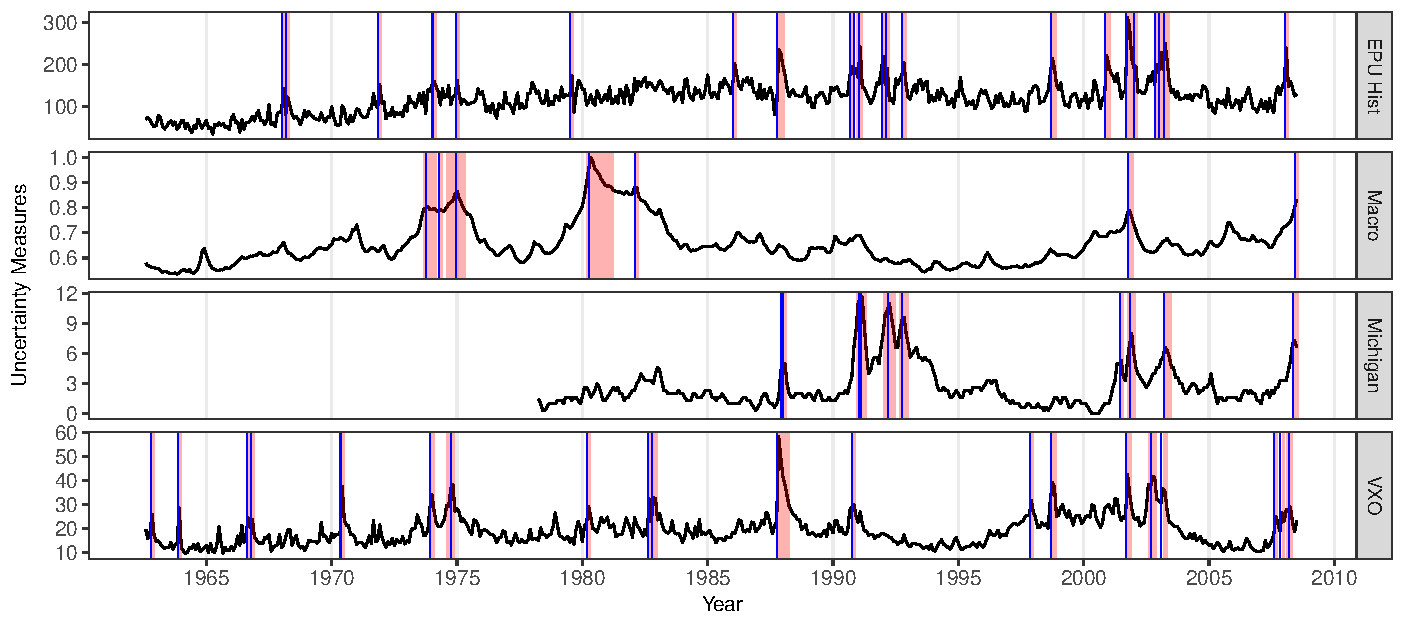
\includegraphics[trim=1cm -1.5cm 0.8cm -0cm, width=1.5\textwidth]{BLOOM_Shocks_plot_combined.pdf}}
      \caption[Comparison of uncertainty measures including 'Bloom-shocks' (facetted).]{Comparison of uncertainty measures including 'Bloom-shocks' (facetted).
      \textit{Note:} Shaded areas denote shock-periods (high uncertainty periods) following \citet{bloom:09} according to the following definition: high uncertainty periods are defined as periods where a series value is more than 1.65 standard deviations above the HP-detrended mean of the series. Data frequencies are monthly. Blue horizontal lines mark months of maximum volatility within a high-uncertainty period (the actual 'Bloom-Shocks'). All series apart from consumer uncertainty series (Michigan Survey) start in July 1962, Michigan Survey in March 1978.}   \label{fig:bloom_shock_all}
\end{figure}
\end{landscape}


\subsection{Exogenous Shocks vs. Endogenous Response}
\label{sec:exoEndoJuradoetal}
Despite showing own variation, the rise of uncertainty in recessions as confirmed by a growing body of literature and our own analysis as suggested by Table~\ref{tab:summary_stats1} is robust to the specific uncertainty measure deployed as a proxy to capture the latent stochastic process of uncertainty. But despite both theoretical and empirical advances that confirm for uncertainty playing a role in business cycles, the question about uncertainty being an exogenous source of business cycle fluctuations or an endogenous response thereof is yet to be solved. As pointed out by \citet[p. 1]{ludvigsonetal:18}, ``[....] the question of causality and the identification of exogenous variation in uncertainty is a long-standing challenge of the uncertainty literature [which] arises in part because there is no single uncertainty model, hence no theoretical consensus on whether the uncertainty that accompanies deep recessions is primarily a cause or effect (or both) of declines in economic activity.'' As we have seen in in our discussion in Section~\ref{sec:UncertaintyandBusinessCyclesRelatedLiterature}, theoretically, most models would point at an adverse effect but even positive effects have been suggested. Even within models pointing ad adverse effects we find various reasoning approaches so that in effect there is ``[...] no single uncertainty theory or all-encompassing structural model'' \citep[p. 5]{ludvigsonetal:18} that could be used to map to the data.\\
\\
\citet{ludvigsonetal:18} identify two issues in the empirical modeling of uncertainty and point at the following shortcomings: First, in a VAR context (results of which in the literature we have reported in Section~\ref{sec:selectedworkindetail} and whose underlying theory we will discuss in greater detail in Section~\ref{sec:IRFsVARversusLocalProj}), the deployed models primarily rely on recursive schemes as an identification strategy whose justification in terms of ordering due to contemporaneous movement of the variables seems sometimes arbitrary and not well grounded.\footnote{\citet{ludvigsonetal:18} also discuss other commonly used identification schemes: sign restrictions, long-run restrictions, IV estimations, etc. Because of ambiguous theoretical signs of the relationships between uncertainty and real activity, the authors conclude that sign restrictions are inappropriate. Similarly they reject IV analysis, stating that it is very difficult to find truly exogenous instruments.} Second, uncertainty stemming from financial markets might play a different role in business cycles than real economic uncertainty, referring to \citet{ngandwright:13} who find that all the post-1982 recessions have their origins in financial market disturbances and that these recessions come along with distinctly different features as recessions where financial uncertainty plays a subordinate role.

To account for these identified issues, \citet{ludvigsonetal:18} suggest a novel identification strategy within an SVAR framework which we will present in the context of our empirical analysis in Section~\ref{sec:EmpiricalAnalysis}.



\begingroup
    \fontsize{8pt}{12pt}\selectfont
    Note to self:
\begin{itemize}
	\item Further, Bloom writes: ``The only historical example of a persistent second-moment shock was the Great Depression, when uncertainty - as measures by share-returns volatility - rose to 130\% of 9/11 levels on average for the 4 years of 1929 to 1932. 
	\item Further, \citet[p. 657]{bloom:09} writes: ``Of course these first- and second-moment shocks differ both in terms of the moments they impact and in terms of their duration: permanent and temporary, respectively. The reason is that the second-moment component of shocks is almost always temporary while the first-moment component tends to be persistent. --> How does Bloom distinguish those shocks empirically? He writes: ``However, in the immediate aftermath of these shocks, distinguishing them will be difficult, as both the first- and second-moment components will generate an immediate drop in employment, investment, etc.'' \\
Further, p. 655: ``All the large macro shocks highlighted in Figure 1 comprise both a first-and second-moment element, suggesting a more realistic simulation would analyze these together.''
	\item They mention: ``The idea of using specific events and/or external variables to identify shocks is not new. Many important studies have used the narrative approach to construct shock series from historical readings of political and economic events.''
\end{itemize}
\endgroup

%%%%%%%%%%%%%%%%%%%%%%%%EMPIRICALANALYSIS%%%%%%%%%%%%%%%%%%%%%%%%%%%
%%%%%%%%%%%%%%%%%%%%%%%%EMPIRICALANALYSIS%%%%%%%%%%%%%%%%%%%%%%%%%%%
%%%%%%%%%%%%%%%%%%%%%%%%EMPIRICALANALYSIS%%%%%%%%%%%%%%%%%%%%%%%%%%%
%%%%%%%%%%%%%%%%%%%%%%%%EMPIRICALANALYSIS%%%%%%%%%%%%%%%%%%%%%%%%%%%
\chapter{Macroeconomic Dynamics}
\label{sec:EmpiricalAnalysis}
\begingroup
    \fontsize{8pt}{12pt}\selectfont
    Note to self:
\begin{itemize}
	\item Unsere empirische Analyse kann als Sensitivitätsanalyse verstanden werden, die zeigt, wie sehr die von Bontempi et al. (2016) erwähnten Fragen eine Rolle im Nachweis empirischer Zusammenhänge spielen: verwendetes Unsicherheitsmaß, Modell (Variablen), Zeitraum, etc!!!
	\item Frage an Hans: Bloom uses various robustness checks for his VARs including different variables sets and ordering and different variable detrending assumptions; how should we incorporate these alternative robustness estimations into our own estimations?
	\item \citet{bontempietal:16} write: ``Findings in the literature suggest that every time uncertainty is modelled within the macroeconomic VAR context, it [largely] displays a significant negative relationship with economic activity, as uncertainty shocks are broadly found to exert a negative impact on output and employment.[...] \\
	However, this key finding is only robust with regard to the uncertainty impact in the short run, whereas in the long run different works have pointed to somewhat heterogeneous output responses:\\
	For example, the results in \citet{bloom:09} sustain the over-shooting effect of a VIX uncertainty shock on real activity: following the shock, the economy suffers in the short term, but in the long run the initial level of output is surpassed. The evidence in Figure 6 of Bachmann et al (2013) suggests that Bloom's over-shooting is more due to the use of the finance-based measure rather than to any genuine uncertainty effect. (\citet{juradoetal:15} argue that Bloom's over-shooting is an artefact in the data mainly due to his HP filtering, since with raw data the over-shooting dynamics vanish.) The latter fact reinforces our caveats about the reliability of measures of macroeconomic uncertainty based solely on financial information, and suggests that researchers need to be careful when proxying uncertainty with these finance-based measures, as they may label certain transitory financial crises as uncertainty shocks.\\
	\citet{juradoetal:15} and \citet{bachmannetal:13} instead utilize forecast-based measures. Their VAR models reveal that the dynamic response of output to uncertainty shocks sharply reduces the level of production with effects that persist well beyond the horizons considered in their exercise (i.e., more than 4-5 years after the shock).\\
	\citet{bakeretal:15} model the economy by slightly reducing the number of variables in Bloom's VAR (from 8 to 5 macroeconomic variables, uncertainty included), and use their news-based economic policy uncertainty index. They report a negative dynamics response of manufacturing production to a shock. However, unlike \citet{juradoetal:15} and \citet{bachmannetal:13}, these output responses are significantly negative for only the first 15-18 months after the shock, before gradually declining to zero, i.e. without overshooting.''
	\item \citet[p. 674]{bloom:09} writes: ``Hence, the simulated response to uncertainty shocks generates a drop, rebound, and longer-run overshoot, much the same as their actual empirical impact.''
	\item \citet[p. 651]{bloom:09} writes: ``What is striking about Figure 12 is the similarity of the size, duration, and time profile of the simulated response to an uncertainty shock compared to the VAR results on actual data shown in Figure 2.''
 	\item as written in the Appendix of \citet[p. 5]{basuandbundick:17}: ``As we discuss in the main text, the Federal Reserve hit the zero lower bound on nominal interest rates at the end of 2008. While we model this outcome rigorously using our theoretical model, it is less clear how to model the stance of monetary policy during our 1986-2014 sample period econometrically. [...] If we use the 1962-2008 sample of Bloom (2009) with the federal funds rate as the measure of monetary policy, our stylized fact remains: Higher uncertainty generates declines in output, consumption, investment, and hours worked.
	\item  In line with the mainstream perspective and for the purpose of this work, we will elaborate below whether or not we can reasonably argue that the measures of uncertainty that we look at can indeed be regarded as exogenous sources of shocks within our empirical model. 
	\item Here in the introduction to the Empirical Analysis I should outline the intuition behind the benchmark-model that we are analyzing (\citet{bloom:09}) which \citet{bachmannetal:13} describe very well in their introduction to Section 2: ``Time-varying uncertainty at the firm level may have economic consequences when there is a degree of irreversibility to firm actions. For a concrete example, suppose that a firm faces fixed costs to adjusting the size of its labor force and/or physical capital stock. Suppose further that there is a mean-preserving spread on the distribution of future demand for the firm's product. With fixed adjustments costs, higher uncertainty over future demand makes new hiring and investment less attractive. The reason for this is intuitive - if a large fixed cost must be paid do adjust the firm'S labor or capital, then there is reason to minimize the number of times this cost must be paid. If the future is very uncertain (in the sense that demand could be either very high or very low relative to the present), then it makes sense to wait until the uncertainty is resolved to undertake new hiring and investment.'' --> ``An increase in uncertainty thus makes inaction relatively more attractive.'' 
\end{itemize}
\endgroup

In this last section we want to study the dynamic relationships between and responses of a set of key macroeconomic variables to innovations (shocks) of the various uncertainty measures which we have introduced in Section~\ref{MeasuringUncertaintyandaHistoricalView}. Various models have been suggested/studied in the literature each of them suggesting a slightly different set of variables to include, a different specification overall and/or ordering with which the variables enter the VAR. We will start with a replication of the baseline VAR($12$)-8\footnote{Our notation 'VAR($p$) - $v$' denotes the number of lags $p$ and the number of variables included $v$.} that \citet{bloom:09} estimated as a support of his theoretical model of the firm to disentangle responses of output and employment to heightened uncertainty in Section~\ref{sec:VAR8}, explore the trajectory of impulse responses by deploying a different estimation technique as suggested by \citet{jorda:05} in Section~\ref{sec:jorda05} and finally try to disentangle cause and effect by deploying SVARs as suggested by \citet{ludvigsonetal:18} in Section~\ref{sec:ludvigsonetal18}.\\
\\
Central to our study of the effects that the models suggest is the dynamic behavior, i.e., the recovery of impulse response functions. Because the approach deployed in a VAR setting differs from that of local projections (direct multistep forecasts), Section~\ref{sec:IRFsVARversusLocalProj} first starts with an outline of the two approaches and establishes under which circumstances impulse responses derived from a VAR are equivalent to impulse responses recovered from local projections.

%\newpage
\section[Impulse Responses in a VAR Setting Versus Local Projections]{Impulse Responses in a VAR Setting Versus Local Projections\footnote{This entire section draws heavily from various sources including ...... LIST ALL THE BOOKS and other resources I have used!}}
\label{sec:IRFsVARversusLocalProj}

\begingroup
    \fontsize{8pt}{12pt}\selectfont
    Leftovers from previous version:
\begin{itemize}
	\item \citet{jorda:05} popularized the idea of computing impulse responses for vector time series based on \textit{local projections} that go without the specification and estimation of the ``[...] unknown true multivariate dynamic system itself'' \citep[p. 1]{jorda:05}. \\
As part of the advantages, \citet{jorda:05}, among others, shows that local projections provide appropriate inference that goes without asymptotic delta-method approximations or numerical techniques, are robust to misspecificaions of the DGP and more easily allow non-linear specifications (\textit{flexible local projection}). The key argument regards the original purpose of time-series models, i.e., forecasting: A (multiple) linear system (like a VAR) is optimally designed for one-period ahead forecasts and will still produce reasonable one-period ahead forecasts under a misspecified model.\footnote{Using the term 'linear projection' to describe a forecast formed from a linear function of past observations as it is the case in traditional time-series forecasting emphasizes the common goal of traditional time-series forecasting versus local projections.} In case of an acute misspecification, however, looking at more distant horizons, misspecification errors are worsened along with the forecast horizon and passed on to the more distant point forecasts. 

Technically, local projections are the result of sequential regressions of a dependent variable shifted several steps ahead, i.e., regressions of the dependent variables at horizon $t+h$ on the set of regressors at time $t$. As such, the method shares many similarities with direct multi-step forecasting techniques.\footnote{See e.g., \citet{marcellinoetal:06} for a comparison of direct and iterated multistep methods in forecasting practice for univariate time series. They describe forecasts based on a multiperiod model (direct forecast) as regressing a multiperiod-ahead value of the dependent variable on current and lagged values of the variable and show that the comparison between iterated (i.e., forecasts derived from time series models) and direct forecasts involve a trade-off between bias and efficiency: iterated methods win with respect to parameter efficiency but produce a compounded bias if the one-step-ahead model is already misspecified. Similarly like \citet{jorda:05} write that the idea of direct multiperiod forecasts (in comparison to iterated forecasts based on a univariate or multivariate time-series models) goes back to at least \citet{cox:61} whereas \citet{weiss:91} established consistency and asymptotic normality of direct forecasts under general conditions. \citet{bhansali:02} provides a review of the literature.} While direct forecasting aims at an optimal multi-step point forecast of the dependent variable, local projections target a consistent estimation of the corresponding impulse response coefficients (which are obviously two interrelated goals).\\
\\
To put Jordá's local projections properly in context with respect to VARs, in what follows we outline some theory regarding VARs which will allow us then to seamlessly introduce local projections into the picture.
\end{itemize}
\endgroup









\paragraph{Estimation of VARs}


\paragraph{Defining Impulse Responses Under Unknown Wold Decomposition}
\citet{jorda:05} outlines that the deployment of the Wold decomposition (i.e., transformation of a VAR into its MA($\infty$) counterpart) to be able to recover the impulse responses is justified under the premise that the estimated model indeed resembles the underlying DGP. To focus on the actual goal of impulse responses in a model-free context, \citet{jorda:05} reverts back to the original definition of impulse responses without reference to the unknown DGP (and hence without knowing the Wold decomposition) as described by \citet{koopetal:96} and \citet{hamilton:94}:\\
\citet{koopetal:96}\footnote{\citet{hamilton:94} uses a similar description.} introduce the (as they call it) \textit{traditional} definition of an impulse response function as the difference between two different realizations of $\vect{y_{t+s}}$ that are identical up to time $t-1$ but diverge in time $t$ so that 
\begin{equation}
	\vect{x_{t-1}'} = (\vect{y_{t-1}^'}, \vect{y_{t-2}^'}, \dots, \vect{y_{t-p}^'})
\end{equation}
is the information received about the system up to date $t-1$. In this setting, one realization assumes that the system was hit by a shock of size $\vect{\delta}$ between $t$ and $t+s$ while the other one (called benchmark) is not impacted between $t$ and $t+s$. Based on this distinction, even if its Wold decomposition does not exist (as mentioned above) the impulse response function can be defined as the difference between the two forecasts
\begin{equation}\label{eq:IRForecast}
\begin{split}
	IRF(t, s, \vect{\delta}) & = \mathbb{E}(\vect{y_{t+s}}|\vect{u_t}=\vect{\delta}; \vect{x_{t-1}}) - \mathbb{E}(\vect{y_{t+s}}|\vect{u_t}=\vect{0};\vect{x_{t-1}}) \\
	& = \vect{\Psi_s \delta} \\
	\text{for} \quad s & = 0, 1, 2, \dots
\end{split}
\end{equation}
where $\mathbb{E}(.|.)$ denotes the best, mean squared error prediction, $\vect{y_t}$ is an $(n \times 1)$ random vector, $\vect{0}$ is of dimension $(n \times 1)$, $\vect{u_t}$ is the $(n \times 1)$ vector of reduced-form disturbances and $\vect{\delta}$ is an $(n \times 1)$ vector containing the respective changes of $\vect{u_t}$ and answers the question: ``What is the effect of a shock of size $\vect{\delta}$ hitting the system at time $t$ on the state of the system at time $t+s$, given that no other shocks hit the system?'' \citep{koopetal:96}. As stated above, the representation of IRFs in Equations~\ref{eq:IRForecast} or \ref{eq:svar10} give the effect to a one-time unit increase to one of the (structural) shocks while holding all else constant. 
\\
\\
Because of the tricky identification of contemporaneous causal relations in a VAR setting, \citet{jorda:05} criticizes the mechanical standard Wold-causal ordering of the elements of $\vect{y_t}$ on which the VAR literature often relies to establish the triangular factorization of the reduced-form variance-covariance matrix $\vect{\Sigma_u}$ and at the same time finds that the ``statistical-based structural identification of contemporaneous causal links'' is a difficult venture.\footnote{An issue we will pick up again in Section~\ref{sec:ludvigsonetal18} when discussing the approach of \citet{ludvigsonetal:18}.}

\paragraph{Estimation of Impulse Responses Under Local Projections}
By referring to Equation~\ref{eq:IRForecast}, \citet[p. 4]{jorda:05} hence abstracts from the technicalities involved in the estimation of impulse responses with VARs (first estimating a reduced-form model, inverting its estimates for the MA($\infty$) - representation, and recursively iterating through the model, etc.) and asserts the optimality of this approach if the specified VAR indeed correctly represents the GDP but stresses that the ``[...] statistical objective in calculating impulse responses is to obtain the best, mean-squared, multi-step predictions'' and instead suggests to directly project the $s$-step ahead forecast $\vect{y_{t+s}}$ onto the linear space generated by $(\vect{y_{t-1}}, \vect{y_{t-2}}, \dots, \vect{y_{t-2}})$ which yields the following specification
\begin{equation} \label{eq:localproj42}
\begin{split}
	\vect{y_{t+s}} = \vect{\alpha_s} + \vect{K_1^{s+1}}\vect{y_{t-1}} + \vect{K_2^{s+1}}\vect{y_{t-2}} + \cdots + \vect{K_p^{s+1}}\vect{y_{t-p}} + \vect{e_{t+s}^s} \\
	\quad \text{for steps} \quad s=0, 1, 2, \dots, h 
\end{split}								
\end{equation}
where $\vect{\alpha_s}$ is an $(n \times 1)$ vector of constants and the $\vect{K_i^{s+1}}$s are matrices of coefficients for each lag $i$ and horizon $s+1$. The collection of $h$ regressions in Equation~\ref{eq:localproj42} together make up the \textit{local projections}, which, written out, amount to the following set of regressions:
\begin{equation} \label{eq:localproj43}
\begin{split}
	\vect{y_{t+1}} & = \vect{\alpha_1} + \vect{K_1^{1+1}}\vect{y_{t-1}} + \vect{K_2^{1+1}}\vect{y_{t-2}} + \cdots + \vect{K_p^{1+1}}\vect{y_{t-p}} + \vect{e_{t+1}^1} \\
	\vect{y_{t+2}} & = \vect{\alpha_2} + \vect{K_1^{2+1}}\vect{y_{t-1}} + \vect{K_2^{2+1}}\vect{y_{t-2}} + \cdots + \vect{K_p^{2+1}}\vect{y_{t-p}} + \vect{e_{t+2}^2} \\
	& \vdots \\
	\vect{y_{t+s}} & = \vect{\alpha_s} + \vect{K_1^{s+1}}\vect{y_{t-1}} + \vect{K_2^{s+1}}\vect{y_{t-2}} + \cdots + \vect{K_p^{s+1}}\vect{y_{t-p}} + \vect{e_{t+s}^s}
\end{split}								
\end{equation}

With respect to Equation~\ref{eq:IRForecast}, impulse responses from the local-linear projections of the specification \ref{eq:localproj42} hence are given by
\begin{equation}\label{eq:IRFLocProjDefinition}
\begin{split}
	IRF(t, s, \vect{\delta}) & = {\hatt{K}_1^s}\vect{\delta}  \\
	\text{for} \quad s & = 0, 1, 2, \dots
\end{split}
\end{equation}
i.e., the estimates ${\hatt{K}_1^s}$s are the impulse response coefficients.\\
\\
We briefly summarize a few further results shown in \citet{jorda:05}: the residuals $e_{t+s}^s$ in Equation~\ref{eq:localproj42} are a moving average of the forecast errors from time $t$ to $t+s$ due to which they are uncorrelated with the regressors that are dated $t-1$ to $t-p$,\footnote{However, due to this \citet{jorda:05} suggests to use heteroskedasticity and autocorrelation consistent estimators for the variance-covariance matrix (see, e.g., \citealp{newest:87}).} the maximum lag $p$ must not be common for each forecast horizon $s$ and consistency does not require that the sequence of $h$ system regressions as written down in Equations~\ref{eq:localproj42} and \ref{eq:localproj43}, respectively, be estimated jointly (meaning that the impulse response for the $jth$ variable in the vector $\vect{y_t}$ can be estimated by means of single regressions of $y_{jt}$ onto the linear space spanned by $(\vect{y_{t-1}}, \vect{y_{t-2}}, \dots, \vect{y_{t-p}})'$. Further, \citet{jorda:05} shows that the point-wise estimation of impulse responses via local projections is more robust to model misspecification resulting from dispensing iterated multistep-forecasts that get compounded along the way in case of misspecification.\\
One of the apparent downsides, however, is that (as pointed out by \citealp{brugnolini:18}), local projections are more data consuming than VARs by consuming data along both the lag ($p$) and lead ($h$) dimension.

\paragraph{Relationship to VARs}
\citet{jorda:05} establishes the relationship between VARs and local projection estimation by proceeding along the following lines:
\begin{enumerate}
	\item Starting from a \textit{pth-order vector autoregression} - VAR(p) (i.e., a reduced-form representation of a VAR)
	\begin{equation} \label{eq:svar24}
	\begin{split}
		\vect{y_t} = \vect{c} + \vect{B_1}\vect{y_{t-1}} + \vect{B_2}\vect{y_{t-2}} + \cdots + \vect{B_p}\vect{y_{t-p}} + \vect{u_t},
	\end{split}								
	\end{equation}	
	under covariance-stationarity the first and second moments are independent of date $t$ so that it is possible to take expectations on both sides of the equation to calculate the mean $\vect{\mu}$ of the process which gives
	\begin{equation} \label{eq:svar25}
	\begin{split}
		\vect{\mu} = \vect{c} + \vect{B_1}\vect{\mu} + \vect{B_2}\vect{\mu}+\cdots + \vect{B_p}\vect{\mu}
	\end{split}								
	\end{equation}	
	after which Equation~\ref{eq:svar24} can be rewritten in terms of deviations from the mean (note that this eliminates the vector of constants $\vect{c}$) which yields
	\begin{equation} \label{eq:svar26}
	\begin{split}
		(\vect{y_t} - \vect{\mu}) = \vect{B_1}(\vect{y_{t-1}} - \vect{\mu}) + \vect{B_2}(\vect{y_{t-2}} - \vect{\mu}) + \cdots + \vect{B_p}(\vect{y_{t-p}} - \vect{\mu}) + \vect{u_t}
	\end{split}								
	\end{equation}	
	\item Any VAR($p$) - process can be rewritten in its $np$-dimensional VAR(1) companion form by defining the stacked vectors $\vect{\xi_t}$, $\vect{v_t}$ and the block matrix $\vect{F}$\footnote{To see this, consider a small reduced-form VAR($2$)-model $\vect{y_t} = \vect{c} + \vect{B_1}\vect{y_{t-1}} + \vect{B_2}\vect{y_{t-2}} + \vect{u_t}$. Applying a transformation that stacks the lags of the VAR($2$) variables in a new VAR($1$) dependent variable (i.e., in our case the dimension of the dependent variable changes from $(n \times 1)$ to $(n2 \times 1)$) and consequently adjust the coefficient matrix which in this example results in $$\begin{bmatrix} \vect{y_t}\\
				\vect{y_{t-1}}
 				\end{bmatrix} = \begin{bmatrix} 
								\vect{c}\\
								\vect{0}
 								\end{bmatrix} + 
									\begin{bmatrix} 
									\vect{B_1} & \vect{B_2}\\
									\vect{I} & \vect{0}
 									\end{bmatrix} \begin{bmatrix} \vect{y_{t-1}}\\
												\vect{y_{t-2}}
 												\end{bmatrix} + 
												\begin{bmatrix} \vect{u_{t}}\\
												\vect{0}
 												\end{bmatrix}$$ with $\vect{I}$ being the identity matrix.		
						}
						
						
						
	\begin{equation} \label{eq:svar27}
	\begin{split}
		\vect{\xi_t}	 \equiv \begin{bmatrix}
    						\vect{y_t}-\vect{\mu}\\
						\vect{y_{t-1}}-\vect{\mu} \\
						\vdots \\
						\vect{y_{t-p+1}}-\vect{\mu}
 						\end{bmatrix}_{np \times 1} \\
		\vect{F} \equiv \begin{bmatrix}
    						\vect{B_1} & \vect{B_2} & \vect{B_3} & \cdots & \vect{B_{p-1}} & \vect{B_p}\\
						\vect{I_n} & \vect{0} & \vect{0} & \cdots & \vect{0} & \vect{0}\\
						\vect{0} & \vect{I_n} & \vect{0} & \cdots & \vect{0} & \vect{0}\\
						\vdots & \vdots & \vdots & \cdots & \vdots & \vdots\\
						\vect{0} & \vect{0} & \vect{0} & \cdots & \vect{I_n} & \vect{0}
 						\end{bmatrix}_{np \times np}\\
		\vect{v_t} \equiv \begin{bmatrix}
    						\vect{u_t} \\
						\vect{0} \\
						\vdots \\
						\vect{0} \\
 						\end{bmatrix}_{np \times 1}
	\end{split}								
	\end{equation}	
	after which the VAR($p$) as denoted in Equation~\ref{eq:svar26} can be rewritten as a VAR(1):\footnote{Note the dimensions of the defined matrices.}
	\begin{equation} \label{eq:svar28}
	\begin{split}
		\vect{\xi_t} = \vect{F}\vect{\xi_{t-1}} + \vect{v_t}
	\end{split}								
	\end{equation}	
	with
	\begin{equation} \label{eq:svar29}
	\begin{split}
		\mathbb{E}[\vect{v_t}\vect{v_{\tau}^'}] & =     \begin{cases}
      												\vect{Q}, & \text{for} \quad t = \tau \\
      												\vect{0}, & \text{otherwise.}
										\end{cases}
	\end{split}
	\end{equation}
	and
	\begin{equation} \label{eq:svar30}
	\begin{split}
		\vect{Q} \equiv \begin{bmatrix}
    						\vect{\Sigma_u} & \vect{0} & \cdots & \vect{0} \\
						\vect{0} & \vect{0} & \cdots & \vect{0} \\
						\vdots & \vdots & \cdots & \vdots \\
						\vect{0} & \vect{0} & \cdots & \vect{0} 
 						\end{bmatrix}
	\end{split}								
	\end{equation}		
	\item Equation~\ref{eq:svar28} implies 
	\begin{equation} \label{eq:svar31}
	\begin{split}
		\vect{\xi_{t+s}}  = \vect{v_{t+s}} + \vect{F}\vect{v_{t+s-1}} + \vect{F}^2\vect{v_{t+s-2}} + \vect{F}^3\vect{v_{t+s-3}} + \cdots + \vect{F}^{s}\vect{v_{t}} + \vect{F}^{s+1}\vect{\xi_{t-1}} 
	\end{split}								
	\end{equation}	
	from which $s$-step ahead forecasts can be computed.
	\item Denoting $\vect{F_{11}^{(j)}}$ as the upper left block of $\vect{F^j}$, with $\vect{F^j}$ being the matrix $\vect{F}$ raised to the $j$th power so that the $(n \times n)$ matrix $\vect{F_{11}^{(j)}}$ indicates rows 1 through $n$ and columns 1 through $n$ of the $(np \times np)$ matrix $\vect{F^j}$, similarly, $\vect{F_{12}^{(j)}}$ denotes the part of $\vect{F_j}$ consisting of rows 1 through $n$ and columns $(n + 1)$ through $2n$. Generally, $\vect{F_{1p}^{(j)}}$ denotes rows 1 through $n$ and columns $[n(p - 1) + 1]$ through $np$ of $\vect{F^j}$, the first $n$ rows of Equation~\ref{eq:svar28} result to
	\begin{equation} \label{eq:svar32}
	\begin{split}
		\vect{y_{t+s}}-\vect{\mu} &  = \\
				       & = \vect{u_t} + \vect{F_{11}^{(1)}}\vect{u_{t+s-1}} + \vect{F_{11}^{(2)}}\vect{u_{t+s-2}} + \vect{F_{11}^{(3)}}\vect{u_{t+s-3}} + \cdots + \vect{F_{11}^{(s)}}\vect{u_{t}} + \\
				       & + \vect{F_{11}^{(s+1)}}(\vect{y_{t-1}}-\vect{\mu}) + \vect{F_{12}^{(s+1)}}(\vect{y_{t-2}}-\vect{\mu}) + \cdots + \vect{F_{1p}^{(s+1)}}(\vect{y_{t-p}}-\vect{\mu})
	\end{split}								
	\end{equation}		
	with $\vect{\Psi_j} = \vect{F_{11}^{(j)}}$. \\
	Under covariance stationarity (i.e., the eigenvalues of $\vect{F}$ all lie inside the unit circle), it holds that $\vect{F^s} \to \vect{0}$ as $s \to \infty$ due to which $\vect{y_t}$ from Equation~\ref{eq:svar24} can be written down in its infinite vector moving-average representation as follows
	\begin{equation} \label{eq:svar33}
	\begin{split}
		\vect{y_t} = \vect{\mu} + \vect{u_t} + \vect{F_{11}^{(1)}}\vect{u_{t-1}} + \vect{F_{11}^{(2)}}\vect{u_{t-2}} + \cdots +  \vect{F_{11}^{(s)}}\vect{u_{t-s}} + \cdots
	\end{split}								
	\end{equation}	
	with the impulse response function given by
	\begin{equation}\label{eq:svar33a}
\begin{split}
	IRF(t, s, \vect{\delta}) & = {\vect{F}_1^s}\vect{\delta}  \\
	\text{for} \quad s & = 0, 1, 2, \dots
\end{split}
\end{equation}
	\item Ultimately, \citet{jorda:05} establishes the relationship between impulse responses calculated via local projections versus impulse responses estimated from a VAR by comparing the two expressions from Equation~\ref{eq:svar32} (slightly rearranged) with Equation~\ref{eq:localproj42}: \\Comparing
		\begin{equation} \label{eq:svar34}
	\begin{split}
		\vect{y_{t+s}} = \vect{\alpha_s} + \vect{K_1^{s+1}}\vect{y_{t-1}} + \vect{K_2^{s+1}}\vect{y_{t-2}} + \cdots + \vect{K_1^{s+1}}\vect{y_{t-p}} + \vect{e_{t+s}^s}\\
	\quad \text{for steps} \quad s=0, 1, 2, \dots, h 
	\end{split}								
	\end{equation}	
	to a slightly rearranged version of Equation~\ref{eq:svar32}
	\begin{equation} \label{eq:svar35}
	\begin{split}
		\vect{y_{t+s}} & = (\vect{I} - \vect{F_{11}^s} - \cdots - \vect{F_{1p}^s})\vect{\mu} + \vect{F_{11}^{s+1}}\vect{y_{t-1}} + \cdots + \vect{F_{1p}^{s+1}}\vect{y_{t-p}} + \\
		& + (\vect{u_{t+s}} + \vect{F_{11}^1}\vect{t_{t+s-1}} + \cdots + \vect{F_{11}^s}\vect{t_{t}})
	\end{split}								
	\end{equation}	
	shows that 
			\begin{equation} \label{eq:svar36}
	\begin{split}
		\vect{\alpha^s} & = (\vect{I} - \vect{F_{11}^s} - \cdots - \vect{F_{1p}^s})\vect{\mu} \\
		\vect{K_1^{s+1}} & = \vect{F_{11}^{s+1}} \quad \text{, and} \\
		\vect{e_{t+s}^s} & = (\vect{u_{t+s}} + \vect{F_{11}^1}\vect{t_{t+s-1}} + \cdots + \vect{F_{11}^s}\vect{t_{t}})
	\end{split}								
	\end{equation}	\begin{equation} \label{eq:svar36}
	\begin{split}
		\vect{\alpha^s} & = (\vect{I} - \vect{F_{11}^s} - \cdots - \vect{F_{1p}^s})\vect{\mu} \\
		\vect{K_1^{s+1}} & = \vect{F_{11}^{s+1}} \quad \text{, and} \\
		\vect{e_{t+s}^s} & = (\vect{u_{t+s}} + \vect{F_{11}^1}\vect{t_{t+s-1}} + \cdots + \vect{F_{11}^s}\vect{t_{t}})
	\end{split}								
	\end{equation}	
	Jordá concludes that when the DGP is indeed a VAR as in expression~\ref{eq:svar24}, Equations~\ref{eq:svar35} and \ref{eq:svar36} show that impulse responses calculated by local projections and via VARs are equivalent. Further, the error terms in the local projection specification $\vect{e_{t+s}^s}$ are a moving average of the forecast errors from time $t$ through $t+s$.
\end{enumerate}

%%%%%%%%%%%%%%%%%%%%%%%RESULTINGSPECIFICATIONS%%%%%%%%%%%%%%%%%%%%%%%%%%
\section{Resulting Specifications}
Based on the explanations above, we will estimate three models:
\begin{enumerate}

\item As our benchmark model, Section~\ref{sec:VAR8} will estimate the baseline VAR from \citet{bloom:09}.\footnote{As part of his robustness checks, \citet{bloom:09} estimates several variants of his baseline model. What we call 'benchmark' here is Bloom's baseline model where all variables apart from the uncertainty measure enter log-detrended.} In particular, the model looks as follows:\\
\\
\citet{bloom:09} estimates a VAR(8)-12\footnote{Using a VAR(p) to describe a system of $n$ endogenous time series processes, i.e., $\vect{y_n}$ implies that $p$ lags are sufficient to summarize all of the dynamic correlations between the elements of $\vect{y_n}$ in the system.} consisting of variables as depicted in vector~\ref{eq:VAR8} (top part) via a recursive scheme (i.e., cholesky decomposition) based on the assumptions that shocks instantaneously influence the stock market (levels and volatility), then move on to prices (wages, the consumer price index (CPI), and interest rates), and finally eventually affect quantities (hours, employment and output). In particular, \citet{bloom:09}'s rationale for including the stock-market levels as the first variable in the ordering is to ensure that the impact of stock-market levels is already controlled for when looking at the impact of volatility shocks (see \citealp[p. 630]{bloom:09}). Further, \citet{bloom:09} detrends all variables that enter the VARs using the HP-filter (\citealp{hodrickandprescott:97}) apart from the uncertainty measure(s).\footnote{In vector~\ref{eq:VAR8} all variables that enter the VAR detrended are marked with a $c$-prefix to indicate that the variable denotes the remaining cycle-component after removal of the trend.}\\
\\
\citet{juradoetal:15} replicate \citet{bloom:09}'s VARs in their contribution, renounce to detrend the variables however, arguing that the HP filter uses information over the entire sample which makes it difficult to interpret the timing of an observation and report results using \citet{bloom:09}'s original detrended variables in their Appendix. We will estimate their this specification as well (low part vector~\ref{eq:VAR8}).

\begin{equation} \label{eq:VAR8}
\begin{split}
\vect{y_t} &  = 
 \begin{bmatrix} 
 		y_{1t} \\
		y_{2t} \\
		y_{3t} \\
		y_{4t} \\
		y_{5t} \\
		y_{6t} \\
		y_{7t} \\
		y_{8t} 
	      \end{bmatrix} = 
 \begin{bmatrix} \text{c-log(S\&P500 Index)} \\ 
				      \textit{uncertainty measure}\\ 
				      \text{c-federal funds rate}\\
				      \text{c-log(wages)}\\
				      \text{c-log(CPI)}\\
				      \text{c-hours}\\
				      \text{c-log(employment)}\\
				      \text{c-log(industrial production)}
	      \end{bmatrix}\\\\
\vect{y_t} & = 
 \begin{bmatrix} 
 		y_{1t} \\
		y_{2t} \\
		y_{3t} \\
		y_{4t} \\
		y_{5t} \\
		y_{6t} \\
		y_{7t} \\
		y_{8t} 
	      \end{bmatrix} = 	      
	      \begin{bmatrix} \text{log(S\&P500 Index)} \\ 
				      \textit{uncertainty measure}\\ 
				      \text{federal funds rate}\\
				      \text{log(wages)}\\
				      \text{log(CPI)}\\
				      \text{hours}\\
				      \text{log(employment)}\\
				      \text{log(industrial production)}
	      \end{bmatrix}
\end{split}
\end{equation}
Including twelve lags in the estimation results in the following reduced-form VAR(8)-12-system to be estimated:
	\begin{equation} \label{eq:VAR8_1}
	\begin{split}
		\vect{y_t} = {\hatt{c}} + {\hatt{B}_1}\vect{y_{t-1}} + {\hatt{B}_2}\vect{y_{t-2}} + \cdots + {\hatt{B}_{12}}\vect{y_{t-12}} + {\hatt{u}_t}
	\end{split}								
	\end{equation}	
with ${\hatt{c}}$ being an $(8 \times n)$ vector of constants, $\vect{y_t}, \vect{y_{t-1}}, \dots, \vect{y_{t-12}}$ being $(8 \times 1)$ vectors, ${\hatt{u}_t}$ being an $(8 \times 1)$ vector and the estimated matrices ${\hatt{B}_1}, {\hatt{B}_2}, \dots, {\hatt{B}_{12}}$ all having dimension $(8 \times 8)$
which details to
	\begin{equation} \label{eq:VAR8_2}
		\begin{split}
		\begin{bmatrix}
    		y_{1,t} \\
    		y_{2,t} \\
		\vdots \\
		y_{8,t}
 		\end{bmatrix} & = 
		\begin{bmatrix}
    		\hattnobf{c}_{{1}} \\
    		\hattnobf{c}_{{2}} \\
		\vdots \\
		\hattnobf{c}_{{8}}
 		\end{bmatrix} + 
		\begin{bmatrix}
    		\hattnobf{b}_{{1,1}_1} & \hattnobf{b}_{{1,2}_1} & \hattnobf{b}_{{1,2}_1} & \cdots & \hattnobf{b}_{{1,8}_1}\\
    		\hattnobf{b}_{{2,1}_1} & \hattnobf{b}_{{2,2}_1} & \hattnobf{b}_{{2,3}_1} & \cdots & \hattnobf{b}_{{2,8}_1}\\
		\vdots & \vdots & \vdots & \cdots & \vdots \\
		\hattnobf{b}_{{8,1}_1} & \hattnobf{b}_{{8,2}_1} & \hattnobf{b}_{{8,3}_1} & \cdots & \hattnobf{b}_{{8,8}_1}\\
 		\end{bmatrix} 
		\begin{bmatrix}
    		y_{1,t-1} \\
    		y_{2,t-1} \\
		\vdots \\
		y_{8, t-1}
 		\end{bmatrix} + \\
		& +
		\begin{bmatrix}
    		\hattnobf{b}_{{1,1}_2} & \hattnobf{b}_{{1,2}_2} & \hattnobf{b}_{{3,1}_2} & \cdots & \hattnobf{b}_{{8,1}_2}\\
    		\hattnobf{b}_{{2,1}_2} & \hattnobf{b}_{{2,2}_2} & \hattnobf{b}_{{2,3}_2} & \cdots & \hattnobf{b}_{{8,2}_2}\\
		\vdots & \vdots & \vdots & \cdots & \vdots \\
		\hattnobf{b}_{{8,1}_2} & \hattnobf{b}_{{8,2}_2} & \hattnobf{b}_{{8,3}_2} & \cdots & \hattnobf{b}_{{8,8}_2}\\
 		\end{bmatrix} 
		\begin{bmatrix}
    		y_{1,t-2} \\
    		y_{2,t-2} \\
		\vdots \\
		y_{8, t-2}
 		\end{bmatrix} +\\
		& + \cdots + \\
		& + 
		\begin{bmatrix}
    		\hattnobf{b}_{{1,1}_{12}} & \hattnobf{b}_{{1,2}_{12}} & \hattnobf{b}_{{3,1}_{12}} & \cdots & \hattnobf{b}_{{8,1}_{12}}\\
    		\hattnobf{b}_{{2,1}_{12}} & \hattnobf{b}_{{2,2}_{12}} & \hattnobf{b}_{{2,3}_{12}} & \cdots & \hattnobf{b}_{{8,2}_{12}}\\
		\vdots & \vdots & \vdots & \cdots & \vdots \\
		\hattnobf{b}_{{8,1}_{12}} & \hattnobf{b}_{{8,2}_{12}} & \hattnobf{b}_{{8,3}_{12}} & \cdots & \hattnobf{b}_{{8,8}_{12}}\\
 		\end{bmatrix} 
		\begin{bmatrix}
    		y_{1,t-12} \\
    		y_{2,t-12} \\
		\vdots \\
		y_{8, t-12}
 		\end{bmatrix}  + 
		\begin{bmatrix}
    		\hattnobf{u}_{1, t} \\
    		\hattnobf{u}_{2, t} \\
		\vdots \\
		\hattnobf{u}_{8, t}
 		\end{bmatrix}. 
	\end{split}								
	\end{equation}	
Off of this specification, impulse responses for industrial production and employment in manufacturing capturing a one-time shock in uncertainty are calculated as outlined in Section~\ref{sec:IRFsVARversusLocalProj}.

\item Based on \ref{eq:localproj43} and \ref{eq:IRFLocProjDefinition}, correspondingly, the specifications for a direct estimation of the impulse responses via local projections that mimic the Bloom VARs look as follows:\\
\\
Because we are interested in the responses of industrial production and employment in manufacturing in particular, as pointed out above, we do not have to jointly estimate the sequence of $h$ system regressions as detailed in Equations~\ref{eq:localproj42} and \ref{eq:localproj43}, respectively. Rather, we regress industrial production (denoted $y_{8,t}$ for the sake of consistency with the naming above) and employment in manufacturing (correspondingly denoted $y_{7, t}$) at each forecast horizon $s$ on the linear space spanned by $(\vect{y_{t-1}}, \vect{y_{t-2}}, \dots, \vect{y_{t-p}})'$. Writing out the system of equations for step $s=1$ only in detail below yields
\begin{equation} \label{eq:localproj46}
\begin{split}
		\begin{bmatrix}
    		y_{1,t+1} \\
    		y_{2,t+1} \\
		\vdots \\
		y_{7, t+1} \\
		y_{8,t+1}
 		\end{bmatrix} & = 
		\begin{bmatrix}
    		\hattnobf{\alpha}_{{1}} \\
    		\hattnobf{\alpha}_{{2}} \\
		\vdots \\
		\hattnobf{\alpha}_{{7}} \\
		\hattnobf{\alpha}_{{8}}
 		\end{bmatrix} + 
		\begin{bmatrix}
    		{\hattnobf{k}_{{1, 1}_1}^{1+1}} & {\hattnobf{k}_{{1, 2}_1}^{1+1}} & {\hattnobf{k}_{{1, 3}_1}^{1+1}} & \cdots & {\hattnobf{k}_{{1, 8}_1}^{1+1}}\\
    		{\hattnobf{k}_{{2, 1}_1}^{1+1}} & {\hattnobf{k}_{{2, 2}_1}^{1+1}} & {\hattnobf{k}_{{2, 3}_1}^{1+1}} & \cdots & {\hattnobf{k}_{{2, 8}_1}^{1+1}}\\
		\vdots & \vdots & \vdots & \cdots & \vdots \\
		{\hattnobf{k}_{{7, 1}_1}^{1+1}} & {\hattnobf{k}_{{7, 2}_1}^{1+1}} & {\hattnobf{k}_{{7, 3}_1}^{1+1}} & \cdots & {\hattnobf{k}_{{7, 7}_1}^{1+1}}\\
		{\hattnobf{k}_{{8, 1}_1}^{1+1}} & {\hattnobf{k}_{{8, 2}_1}^{1+1}} & {\hattnobf{k}_{{8, 3}_1}^{1+1}} & \cdots & {\hattnobf{k}_{{8, 8}_1}^{1+1}}
 		\end{bmatrix} 
		\begin{bmatrix}
    		y_{1,t-1} \\
    		y_{2,t-1} \\
		\vdots \\
		y_{7, t-1} \\
		y_{8, t-1}
 		\end{bmatrix} + \\
		& +
		\begin{bmatrix}
    		{\hattnobf{k}_{{1, 1}_2}^{1+1}} & {\hattnobf{k}_{{1, 2}_2}^{1+1}} & {\hattnobf{k}_{{1, 3}_2}^{1+1}} & \cdots & {\hattnobf{k}_{{1, 8}_2}^{1+1}}\\
    		{\hattnobf{k}_{{2, 1}_2}^{1+1}} & {\hattnobf{k}_{{2, 2}_2}^{1+1}} & {\hattnobf{k}_{{2, 3}_2}^{1+1}} & \cdots & {\hattnobf{k}_{{2, 8}_2}^{1+1}}\\
		\vdots & \vdots & \vdots & \cdots & \vdots \\
		{\hattnobf{k}_{{7, 1}_2}^{1+1}} & {\hattnobf{k}_{{7, 2}_2}^{1+1}} & {\hattnobf{k}_{{7, 3}_2}^{1+1}} & \cdots & {\hattnobf{k}_{{7, 8}_2}^{1+1}}\\
		{\hattnobf{k}_{{8, 1}_2}^{1+1}} & {\hattnobf{k}_{{8, 2}_2}^{1+1}} & {\hattnobf{k}_{{8, 3}_2}^{1+1}} & \cdots & {\hattnobf{k}_{{8, 8}_2}^{1+1}}
 		\end{bmatrix} 
		\begin{bmatrix}
    		y_{1,t-2} \\
    		y_{2,t-2} \\
		\vdots \\
		y_{7, t-2} \\
		y_{8, t-2}
 		\end{bmatrix} +\\
		& + \cdots + \\
		& + 
		\begin{bmatrix}
    		{\hattnobf{k}_{{1, 1}_{12}}^{1+1}} & {\hattnobf{k}_{{1, 2}_{12}}^{1+1}} & {\hattnobf{k}_{{1, 3}_{12}}^{1+1}} & \cdots & {\hattnobf{k}_{{1, 8}_{12}}^{1+1}}\\
    		{\hattnobf{k}_{{2, 1}_{12}}^{1+1}} & {\hattnobf{k}_{{2, 2}_{12}}^{1+1}} & {\hattnobf{k}_{{2, 3}_{12}}^{1+1}} & \cdots & {\hattnobf{k}_{{2, 8}_{12}}^{1+1}}\\
		\vdots & \vdots & \vdots & \cdots & \vdots \\
		{\hattnobf{k}_{{7, 1}_{12}}^{1+1}} & {\hattnobf{k}_{{7, 2}_{12}}^{1+1}} & {\hattnobf{k}_{{7, 3}_{12}}^{1+1}} & \cdots & {\hattnobf{k}_{{7, 8}_{12}}^{1+1}}\\
		{\hattnobf{k}_{{8, 1}_{12}}^{1+1}} & {\hattnobf{k}_{{8, 2}_{12}}^{1+1}} & {\hattnobf{k}_{{8, 3}_{12}}^{1+1}} & \cdots & {\hattnobf{k}_{{8, 8}_{12}}^{1+1}}
 		\end{bmatrix} 
		\begin{bmatrix}
    		y_{1,t-12} \\
    		y_{2,t-12} \\
		\vdots \\
		y_{7, t-12} \\
		y_{8, t-12}
 		\end{bmatrix} + 
		\begin{bmatrix}
    		\hattnobf{e}_{1, t+1} \\
    		\hattnobf{e}_{2, t+1} \\
		\vdots \\
		\hattnobf{e}_{7, t+1} \\
		\hattnobf{e}_{8, t+1}
 		\end{bmatrix}. 
\end{split}								
\end{equation}
Focussing on rows $7$ and $8$ only (the regressions for industrial production and employment in manufacturing) gives us the two regressions that have to be estimated for each $s = 1, 2, \dots, h$.

\begin{equation} \label{eq:localproj46}
\begin{split}
		\begin{bmatrix}
		y_{7, t+s} \\
		y_{8,t+s}
 		\end{bmatrix} & = 
		\begin{bmatrix}
		\hattnobf{\alpha}_{{7}} \\
		\hattnobf{\alpha}_{{8}}
 		\end{bmatrix} + 
		\begin{bmatrix}
		{\hattnobf{k}_{{7, 1}_1}^{1+1}} & {\hattnobf{k}_{{7, 2}_1}^{1+1}} & {\hattnobf{k}_{{7, 3}_1}^{1+1}} & \cdots & {\hattnobf{k}_{{7, 7}_1}^{1+1}}\\
		{\hattnobf{k}_{{8, 1}_1}^{1+1}} & {\hattnobf{k}_{{8, 2}_1}^{1+1}} & {\hattnobf{k}_{{8, 3}_1}^{1+1}} & \cdots & {\hattnobf{k}_{{8, 8}_1}^{1+1}}
 		\end{bmatrix} 
		\begin{bmatrix}
    		y_{1,t-1} \\
    		y_{2,t-1} \\
		\vdots \\
		y_{7, t-1} \\
		y_{8, t-1}
 		\end{bmatrix} + \\
		& +
		\begin{bmatrix}
		{\hattnobf{k}_{{7, 1}_2}^{1+1}} & {\hattnobf{k}_{{7, 2}_2}^{1+1}} & {\hattnobf{k}_{{7, 3}_2}^{1+1}} & \cdots & {\hattnobf{k}_{{7, 8}_2}^{1+1}}\\
		{\hattnobf{k}_{{8, 1}_2}^{1+1}} & {\hattnobf{k}_{{8, 2}_2}^{1+1}} & {\hattnobf{k}_{{8, 3}_2}^{1+1}} & \cdots & {\hattnobf{k}_{{8, 8}_2}^{1+1}}
 		\end{bmatrix} 
		\begin{bmatrix}
    		y_{1,t-2} \\
    		y_{2,t-2} \\
		\vdots \\
		y_{7, t-2} \\
		y_{8, t-2}
 		\end{bmatrix} +\\
		& + \cdots + \\
		& + 
		\begin{bmatrix}
    		{\hattnobf{k}_{{7, 1}_{12}}^{1+1}} & {\hattnobf{k}_{{7, 2}_{12}}^{1+1}} & {\hattnobf{k}_{{7, 3}_{12}}^{1+1}} & \cdots & {\hattnobf{k}_{{7, 8}_{12}}^{1+1}}\\
		{\hattnobf{k}_{{8, 1}_{12}}^{1+1}} & {\hattnobf{k}_{{8, 2}_{12}}^{1+1}} & {\hattnobf{k}_{{8, 3}_{12}}^{1+1}} & \cdots & {\hattnobf{k}_{{8, 8}_{12}}^{1+1}}
 		\end{bmatrix} 
		\begin{bmatrix}
    		y_{1,t-12} \\
    		y_{2,t-12} \\
		\vdots \\
		y_{7, t-12} \\
		y_{8, t-12}
 		\end{bmatrix} + 
		\begin{bmatrix}
    		\hattnobf{e}_{7, t+s} \\
		\hattnobf{e}_{8, t+s}
 		\end{bmatrix}. 
\end{split}								
\end{equation}

\item The third and last specification we want to estimate is based on work by \citet{ludvigsonetal:18}. As introduced in Section~\ref{sec:exoEndoJuradoetal}, the authors suggest a novel identification scheme in an attempt to model causalities within an (S)VAR-framework. Because their model needs a separate dedicated explanation, Section~\ref{sec:ludvigsonetal18} will discuss both their empirical approach and the resulting specification.

\end{enumerate}


\section{The Benchmark Model: Recursive VAR(12)-8 following \citet{bloom:09}}
\label{sec:VAR8}


\begingroup
    \fontsize{8pt}{12pt}\selectfont
    Note to self:
\begin{itemize}
	\item The assumptions underlying Bloom's (recursive) VARs are very strong (although he claims that his VARs are insensitive to variable ordering in the Appendix!)
	\item We should write down the VAR-equation that we are estimating (just for the sake of completeness!) --> See the notation in Pfaff!
\end{itemize}
\endgroup

\begin{figure}[!h]
   \centering
   \setlength\fboxsep{0pt}
   \setlength\fboxrule{0pt}
   \fbox{\includegraphics[trim=0.1cm -2.0cm -0.5cm 0.0cm, width=0.9\textwidth]{var8_plot_all_HP_until2008.pdf}}
      \caption[Impulse Response Functions of Production and Employment from Estimations of VAR-8 following \citet{bloom:09} using all uncertainty measures.]{Impulse Response Functions of Production and Employment from Estimations of VAR-8 following \citet{bloom:09} using all uncertainty measures. Variables enter the VAR-8 according to \ref{eq:VAR8}.\\
      \textit{Note:}  The light and dark areas represent 95\% and 68\% bootstrapped confidence bands (100 replications), respectively. The data are monthly and span the period 1962:07-2008:06 for the Bloom-Shock and VXO/volatility series, 1978:02-2008:06 for the MSoC uncertainty series, 1975:01-2008:06 for the EPU and 1962:07-2008:06 for the Macro Uncertainty Index (both $h=1$ and $h=12$).}   \label{fig:VAR8_HP_until2008}
\end{figure}

\begin{figure}[!h]
   \centering
   \setlength\fboxsep{0pt}
   \setlength\fboxrule{0pt}
   \fbox{\includegraphics[trim=0.1cm -2.0cm -0.5cm 0.0cm, width=0.9\textwidth]{var8_plot_all_NoHP_until2008.pdf}}
      \caption[Impulse Response Functions of Production and Employment from Estimations of a modified version of the VAR-8 following \citet{bloom:09} using all uncertainty measures.]{Impulse Response Functions of Production and Employment from Estimations of a modified version of the VAR-8 \citet{bloom:09} using all uncertainty measures. Variables enter the VAR-8 according to \ref{eq:VAR8}.\\
       \textit{Note:} The light and dark areas represent 95\% and 68\% bootstrapped confidence bands (100 replications), respectively. The data are monthly and span the period 1962:07-2008:06 for the Bloom-Shock and VXO/volatility series, 1978:02-2008:06 for the MSoC uncertainty series, 1975:01-2008:06 for the EPU and 1962:07-2008:06 for the Macro Uncertainty Index (both $h=1$ and $h=12$).}   \label{fig:VAR8_NoHP_until2008}
\end{figure}

To summarize the dynamic relationship between the variables in our equation system, Figure~\ref{fig:VAR8_HP_until2008} shows the (orthogonalized) impulse response functions (IRFs) to orthogonal shocks (i.e., uncorrelated) created from a Cholesky decomposition for the VAR-8 setting according to \citet{bloom:09}'s original contribution (i.e., all variables apart from the uncertainty measures are detrended). While \citet{bloom:09} solely considers the VXO/volatility-series (and derived shock-measures in various flavors - one of which, the month with the maximum volatility in a series of months with extraordinarily high volatility, we call 'Bloom-Shock' here) as his uncertainty measure with its effect on industrial production (as a proxy for output) and employment, in the spirit of \citet{juradoetal:15} and \citet{bontempietal:16} we here report a full bank of IRFs for the selection of popularized uncertainty measures we have discussed in Section~\ref{sec:MeasuringUncertainty}: the original 'Bloom-shock' and the VXO/volatility-series (as used by \citealp{bloom:09}), the MSoC (as used by \citealp{leducandliu:16}), the EPU (as used by \citealp{bakeretal:15}), the GTU (as used by \citealp{bontempietal:16} and \citealp{castelnuovoandtran:17}) and finally the macro uncertainty index as introduced by \citet{juradoetal:15}.


have to write into the caption that the length of the availability of the uncertainty measure is the limiting factors in all VARs (so for the macro uncertainty index, accordingly all data runs from 1960 until 2018, for the EPU from 1985 until 2018, for the GTU from 2004 to 2018 etc., etc.!!!)



A good sentence: 'The effect on impact, in contrast, is small.' 
Ein Satz aus Bachmann, den ich für meine eigene Arbeit verwenden sollte: "The next sectino discusses the wait-and-see mechanism and delivers a benchmark against which we compare our empirical results." (p. 4) --> Then I can replicate the results from Bloom and then show the results that local projections would produce.\\
\\
Note to self: \citet{bachmannetal:13} write on p. 5: ``In this section we give a brief overview of the ``wait-and-see'' mechanism that might give rise to uncertainty-driven fluctuations. In addition to providing a benchmark against which we can compare our empirical results, this exercise will also serve to motivate the use of high-frequency, sectoral data in examining the impact of uncertainty on economic activity.''\\
Another sentence that \citet{bachmannetal:13} use on p. 6: ``Figure 2 provides an example of an impulse response of output to an increase in uncertainty, replicated from the model in \citet{bloom:09}.


%%%%%%%%%%%%%%%%%%%%%%%%%%%%LOCALPROJECTIONS%%%%%%%%%%%%%%%%%%%%%%%%%%
\section{Alternative Estimations I: Local Projections following \citet{jorda:05}}
\label{sec:jorda05}

Potential endogeneity in the VAR specifications from Section~\ref{sec:VAR8} is an important issue in our attempts to disentangle the real effects of uncertainty, meaning that uncertainty itself may be a function of the business cycle. As discussed in Section~\ref{sec:exoEndoJuradoetal}, the VARs employed in the literature might not be capable of adequately separating cause and effect (--> go in a little more detail here!!!). IRFs are sensitive to misspecifications in the underlying data generating process. Instead of relying on the recursive scheme of a reduced-form VAR-system to estimate IRFs, it is possible to estimate the IRFs directly from the data by regressing future values of the variable of interest on current values of the set of control variables. \\
\\
For the series of regressions we look five years ahead, i.e., estimate 61 regressions using monthly data (starting to count at $h=0$). And because the $e_{t+s}$ will be autocorrelated, the standard errors must be HAC, i.e. \textit{hereoskedasticity and autocorrelation consistent}.\\
The data-sources are described in Appendix~\ref{sec:data}



Figures \ref{fig:locproj_plot_all_HP_until2008} and \ref{fig:locproj_plot_all_NoHP_until2008} show the responses of industrial production and employment in production when the responses are estimated via local projections. In particular, Figure~\ref{fig:locproj_plot_all_HP_until2008} \\
\\
\begingroup
    \fontsize{8pt}{12pt}\selectfont
    Note to self:
\begin{itemize}
	\item as compared to \citet{bloom:09}, we already see a different pattern (BUT: we have not yet fully 'translated' the model or replicated the data-generating process that \citet{bloom:09} assumes (see next point below).\\
	In particular, as formulated by \citet{bachmannetal:13}, 'we find that innovations to business uncertainty are associated with small and slowly-building reductions in economic activity'. 
	\item guter Satz aus \citet{bachmannetal:13}, p. 15: ``Figure 3 provides corroborating evidence with a different measure of sectoral economic activity.'' 
	\item \citet{bachmannetal:13}, p. 17: ``Wait-and-see theories of the transmission from uncertainty shocks to business cycles emphasize hiring and firing frictions. If the 'wait-and-see' - channel were important, we would observe a large reduction in employment followed by a quick recovery in response to an uncertainty shock, similarly to the output response in Figure 2 in Section 2 (the Bloom-figure).''
	\item weitere guter Satz aus \citet{bachmannetal:13}, p. 17: ``However, the response of manufacturing employment is rather consistent with our other results: it moves little on impact, followed by a period of sustained reductions, with no obvious tendency for reversion, even at very long horizons.'' \\
	Note to self: contrary to their finding, we DO FIND A TENDENCY FOR REVERSION AT THE LONG HORIZON!
	\item bezüglich das DGP: wie sollte unsere Spezifikation aussehen um möglichst nahe an den von Bloom unterstellten DGP ranzukommen? Mit anderen Worten: Wie 'übersetzt' man einen VAR in local projections?
\end{itemize}
\endgroup

\begin{figure}[!h]
   \centering
   \setlength\fboxsep{0pt}
   \setlength\fboxrule{0pt}
   \fbox{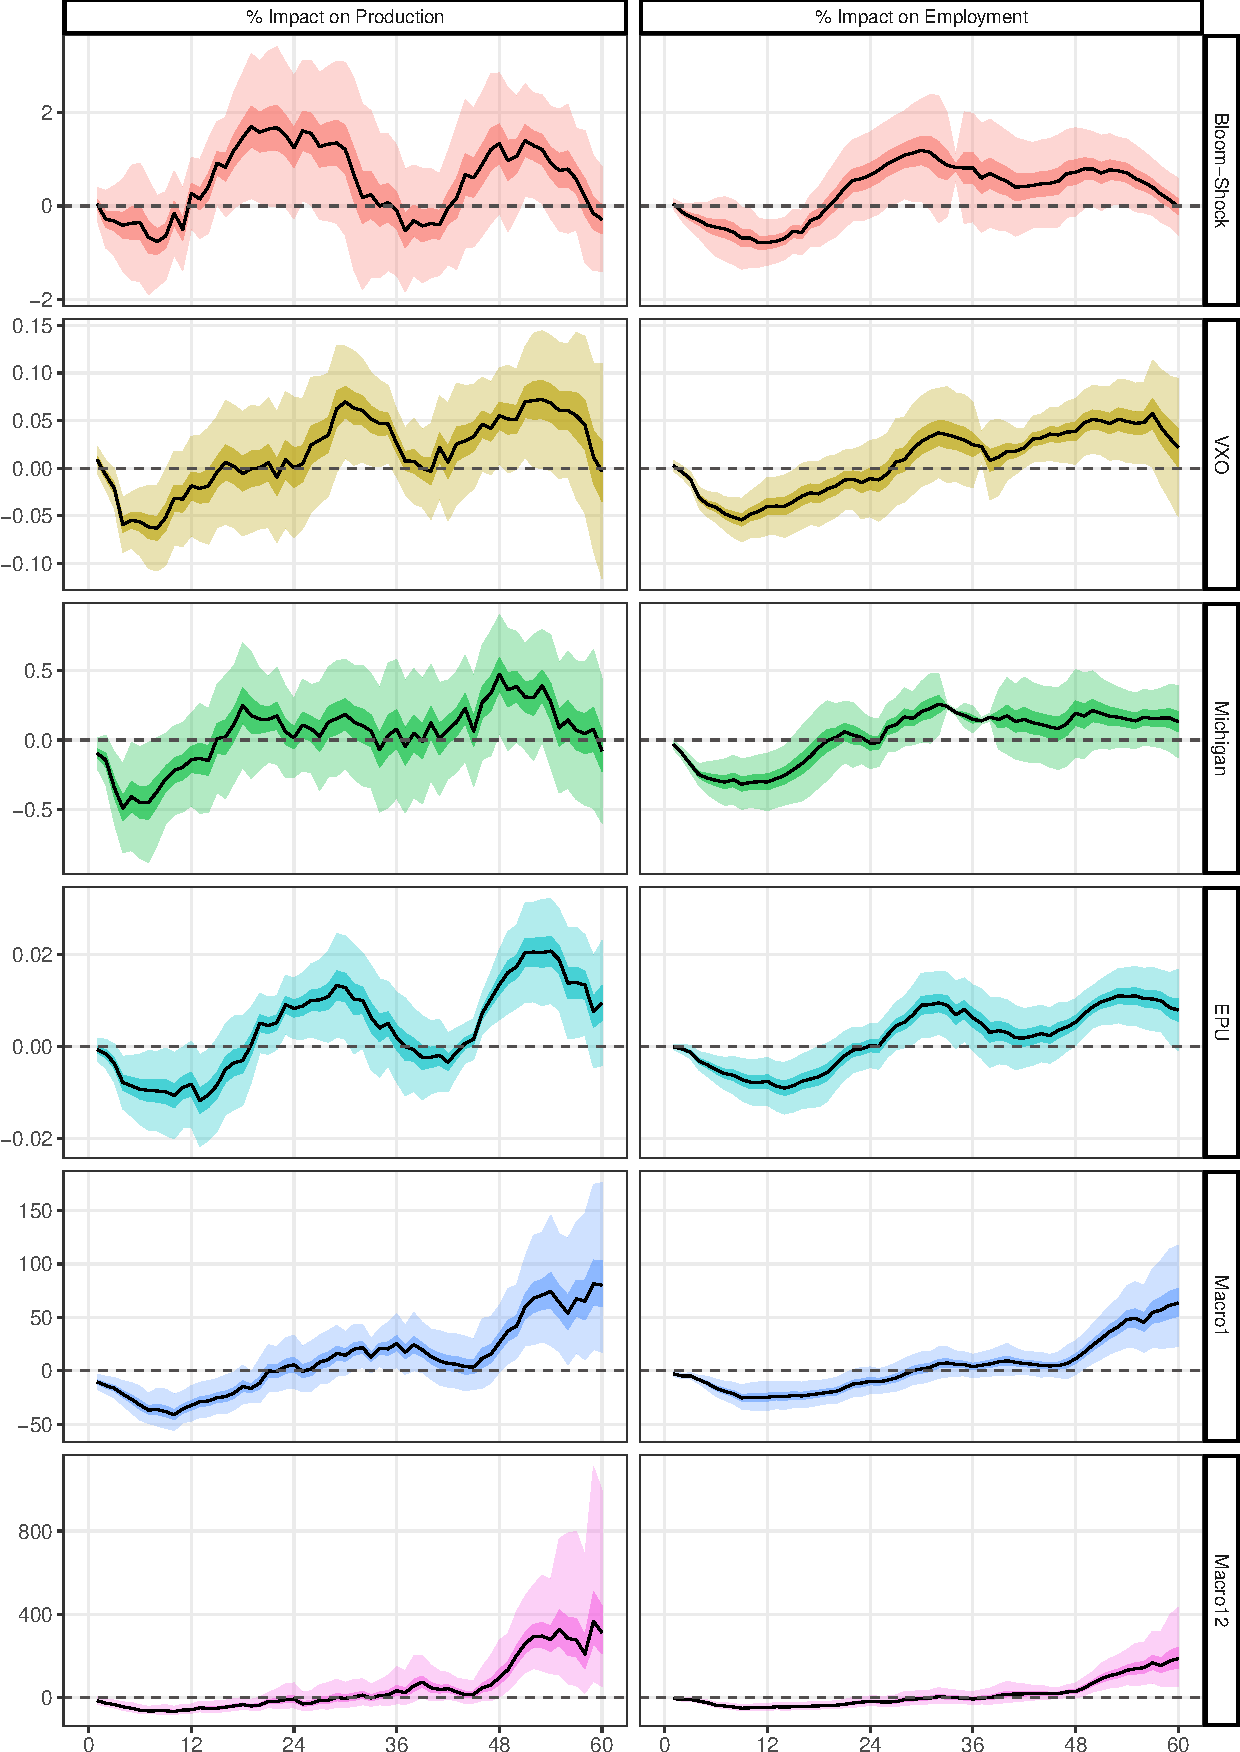
\includegraphics[trim=0.1cm -1cm -0.5cm 0.9cm, width=0.9\textwidth]{locproj_plot_all_HP_until2008.pdf}}
      \caption[Local projection estimations showing the impact of an uncertainty shock on industrial production and employment in manufacturing. All variables apart from uncertainty measures log-detrended.]{Local projection estimations showing the impact of an uncertainty shock on industrial production and employment in manufacturing. All variables apart from uncertainty measures log-detrended.
      \textit{Note:} Dashed lines are 1 standard-error bands around the response to a volatility shock.}
   \label{fig:locproj_plot_all_HP_until2008}
\end{figure}


\begin{figure}[!h]
   \centering
   \setlength\fboxsep{0pt}
   \setlength\fboxrule{0pt}
   \fbox{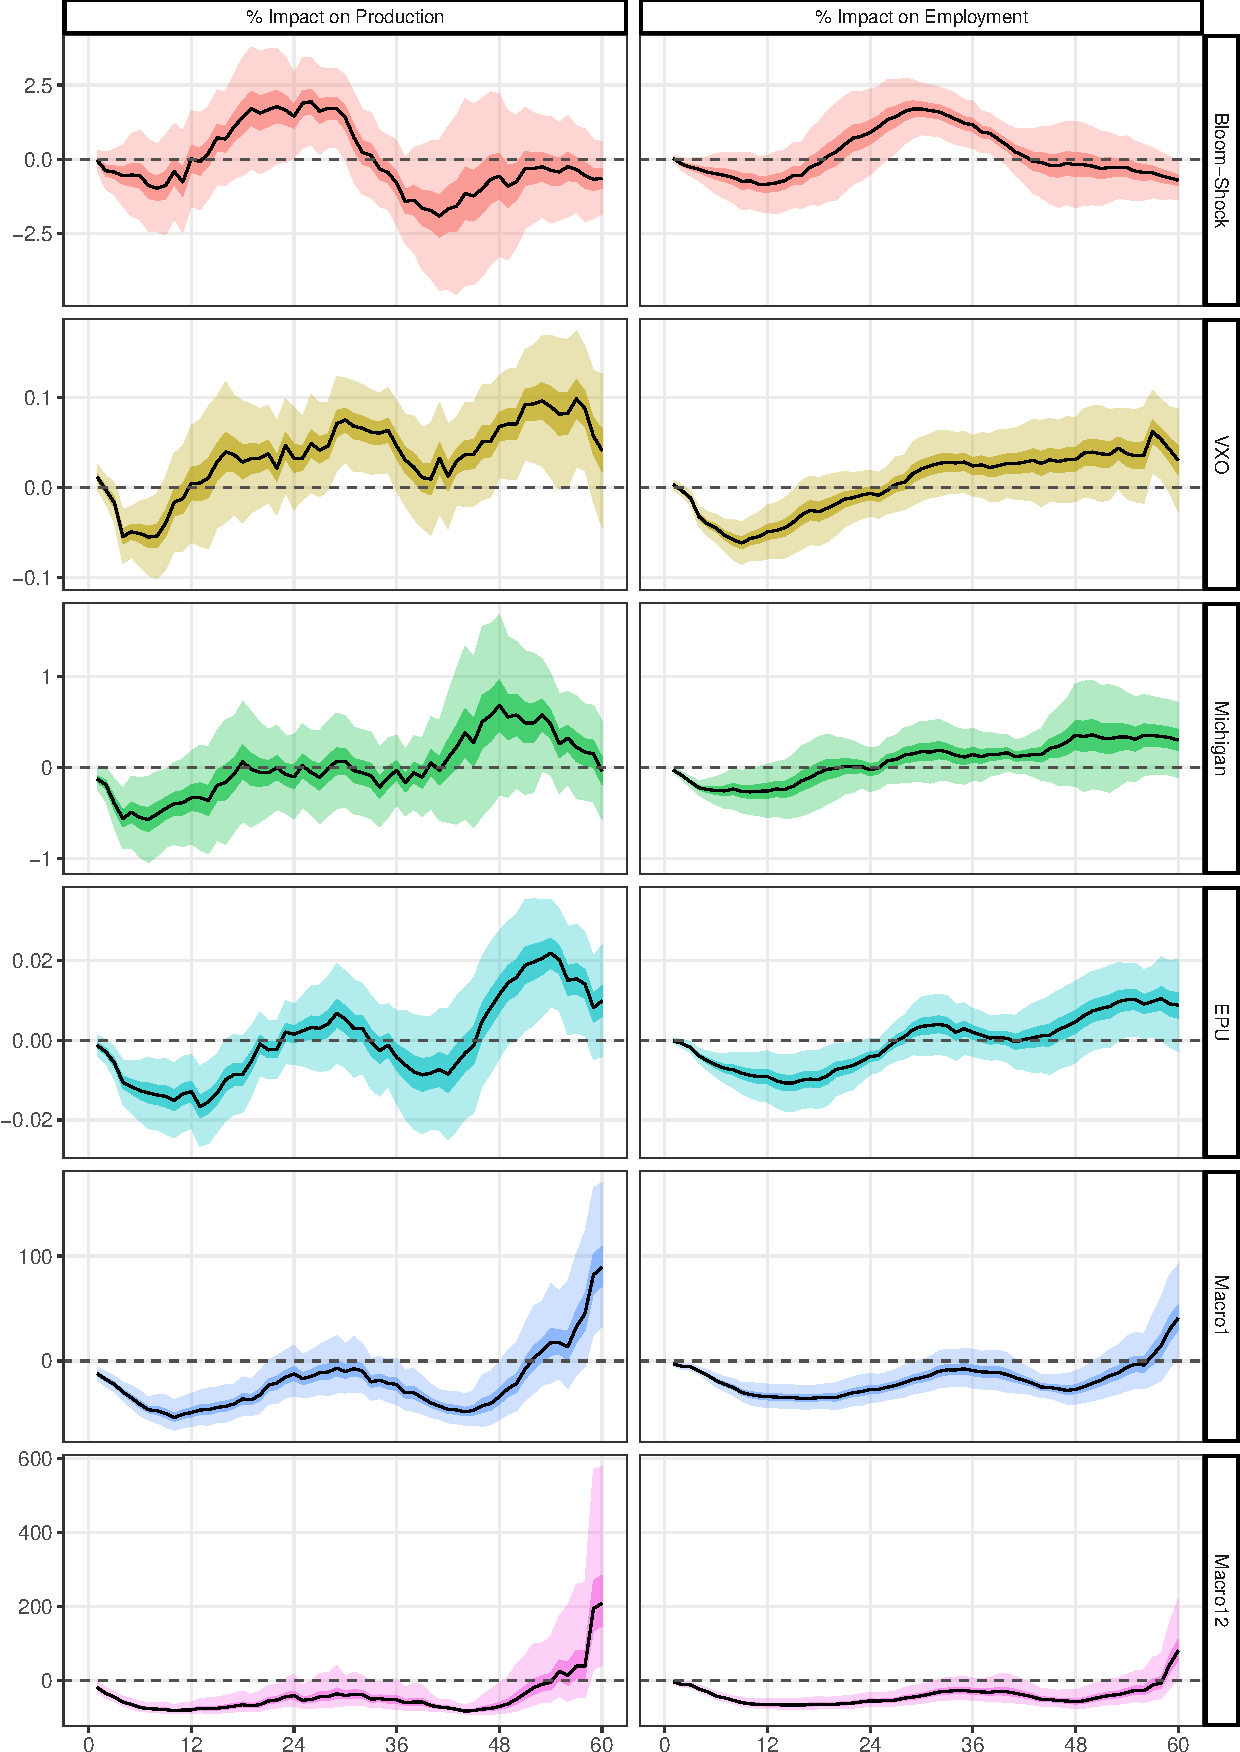
\includegraphics[trim=0.1cm -1cm -0.5cm 0.9cm, width=0.9\textwidth]{locproj_plot_all_NoHP_until2008.pdf}}
      \caption[Local projection estimations showing the impact of an uncertainty shock on industrial production and employment in manufacturing. All variables apart from uncertainty measures enter as logs.]{Local projection estimations showing the impact of an uncertainty shock on industrial production and employment in manufacturing. All variables apart from uncertainty measures enter as logs.
      \textit{Note:} Dashed lines are 1 standard-error bands around the response to a volatility shock.}
   \label{fig:locproj_plot_all_NoHP_until2008}
\end{figure}


\begingroup
    \fontsize{8pt}{12pt}\selectfont
    Note to self:
\begin{itemize}  
	\item ``Real GDP has the virtue of being the broadest indicator of real economic activity. Its downside is that it is difficult to measure [...]. For this reason, we also consider two other indicators: industrial production and the unemployment rate. Industrial production has the benefit of being relatively straightforward to measure; unemployment has the benefit of being perhaps the closest to a purely cyclical indicator.'' (Romer \& Romer, p. 3092)
	\item Footnote 17 in \citet{romandrom:17}: ``The impulse response functions in Figure 4 are estimated using the Jordà local projection method. Figure C2 of online Appendix C shows that the results estimated using a conventional vector autoregression are virtually identical.'' --> should we include a comparison with Bloom's VAR?
	\item \citet[p. 3096]{romandrom:17}: ``To do this, we run the same regression as in equation (1), but with our new measure of financial distress as the dependent variable. Since by construction the response of distress to itself is one at t = 0, we only estimate the regression for horizons 1 to 10. This analysis shows that distress is very serially correlated, particularly at near horizons. This finding suggests that some of the near-term persistence we find in the negative aftermath of financial distress is likely due to persistence in distress itself. It is not necessarily that financial crises have long-lasting effects, but rather that crises themselves tend to last for a while. This possibility [...] is analyzed further in Section III.''
	\item \citet[p. 3097]{romandrom:17}: ``Given that our new series on financial distress differs in important ways from existing crisis chronologies, it is useful to compare our findings for the average aftermath of financial crises with those estimated using the other series.'' --> We can use this approach similarly by using various uncertainty measures in our regressions as alternative and compare the impulse-response functions.
	\item \citet[p. 3099]{romandrom:17}, \textit{Dealing with Heteroskedasticity}: ``The first issue is possible differences in the variance of the residuals across countries. Economic activity is typically much more volatile in the less developed countries in our sample (such as Greece and Turkey), and in the smaller countries. It is plausible to think that the variances of the residuals in equation (1) also vary systematically by country. \\
	--> Taking into account heteroskedasticity in the residuals has a substantial impact on the estimates. Though the time pattern of the decline in GDP is relatively unchanged, the maximum decline is reduced by about one-third.''
	\item \citet[p. 3010]{romandrom:17}: ``In a related exercise, we also consider alternatives to conventional standard errors. In addition to heteroskedasticity of the residuals, there may also be serial correlation due to the overlapping structure of the residuals. We therefore experiment with both heteroskedasticity-consistent standard errors, and two forms of heteroskedasticity- and serial-correlation-corrected standard errors. Table C1 of online Appendix C shows that the alternative standard errors are typically about 30 to 50 percent larger than conventional standard errors. Thus, using the alternatives reduces the statistical significance of the estimated negative aftermath of a financial crisis substantially. Nonetheless, the estimates for GDP remain statistically significant at standard levels at all horizons.''
	\item \citet[p. 15]{ramzub:18}: ``The only complication associated with the Jordà method is the serial correlation in the error terms induced by the successive leading of the dependent variable. Thus, we use the Newey-West correction for our standard errors \citep{newest:87}.''
	\item \citet[p. 16]{ramzub:18}: ``Later, we will be comparing our baseline estimated to those from a threshold VAR." (--> This is something that we can maybe do as well; see a comment added above already!)
	\item \citet[p. 23]{ramzub:18}, footnote 20: ``We only estimate multipliers out five years because the Jordà method is less reliable at long horizons.''
	\item When it comes to describing the data sources I should have a look at the way how \citet{ramzub:18} explain each series in the Appendix.
	\item \citet[p. 17]{ramey:16}: ``If the VAR adequately captures the data generating process, this method is optimal at all horizons. If the VAR is misspecified, however, then the specification errors will be compounded at each horizon. To address this problem, Jordà (2005) introduced a \textit{local projection} method for estimating impulse responses.''
	\item \citet[p. 18]{ramey:16}: ``The control variables need not include the other $Y's$ as long as $\epsilon_{1t}$ is exogenous to those other $Y$'s. Typically, the control variables include deterministic terms (constant, time trends), lags of the $Y_i$, and lags of other variables that are necessary to "mop up''; \\
	One estimates a separate regression for each horizon and the control variables do not necessarily need to be the same for each regression. Note that except for horizon $h=0$, the error term $\xi_{t+h}$ will be serially correlated because it will be a moving average of the forecast errors from $t$ to $t+h$. Thus, the standard errors need to incorporate corrections for serial correlation, such as a \citep{newest:87} correction.
	\item \citet[p. 37]{ramey:16}: The term ``troughs'' is very often used in the context of impulse response functions. Here an example sentence: ``Industrial production begins to fall in the next month and roughs 21 months later.'' Literally translated it means "tief fallen" (auf sein tiefstes Niveau fallen).\\
	Another interesting expression is used on p. 39: ``[...] until they bottom out during the fourth year after the shock.''
	\item \citet[p. 45]{ramey:16}: ``Why does the Jordà method give such different estimates from the proxy SVAR?'' --> This is a question that I could actually elaborate on to possibly also compare our results investigating uncertainty using the Jordà method as opposed to the VAR that Bloom uses in his paper.
	\item In the presentation on the following web-page \url{http://www.datavis.ca/courses/RGraphics/R-Graphics1.pdf} on p. 35 I found an interesting way of plotting regression estimates! (instead of tables with standard errors, we plot the coefficients and confidence bands which let's the viewer immediately understand whether a coefficient is significantly different from zero or not.
\end{itemize}
\endgroup




\paragraph{Robustness Checks: Alternative Uncertainty Measures}
This part provides results from a large number of robustness exercises designed to check the sensitivity of our results to various assumptions. (this sentence is formulated like this by \citet{juradoetal:15}).

\paragraph{Interpretation of Results}
\begingroup
    \fontsize{8pt}{12pt}\selectfont
    Note to self:
\begin{itemize}
	\item \citet[p. 1181]{juradoetal:15} write: ``While we find that increases in uncertainty are associated with large declines in real activity, we caution that our results are silent on wehther uncertainty is the cause or effect of such declines. Our goal is to develop a defensible measure of time-varying macro uncertainty that can be tracked over time and related to fluctuations in real activity and asset markets. Our estimates do, however, imply that the economy is objectively less predictable in recessions thatn it is in normal times. This result is not a statement about changing subjective perceptions of uncertainty in recessions as compared to booms. Any theory for which uncertainty is entirely the effect of recessions would need to be consistent with these basic findings.
	\item \item \citet[p. 1596/1597]{bakeretal:15} write:  ``Although our results are not necessarily causal, one plausible interpretation of our micro and macro evidence is that policy uncertainty retards investment, hiring, and growth in policy-sensitive sectors like defense, finance, healthcare, and construction, and these sectors are important enough for policy uncertainty to matter at the aggregate level.'' --> \\
	In this report, on p. 20, the authors write: \\
	*``A basic challenge for policymakers is thus to move away from an incremental approach to policymaking and address the many downside risks to global activity with strong medium-term fiscal and structural reform programs in order to rebuild confidence. In the euro area, action is also needed to address the current crisis and, over the medium term, to complete the EMU. \\
	*Fiscal adjustment has become necessary in many
cases to strengthen confidence in sovereign balance
sheets and in many other cases because the prospects
for future potential output—and hence revenue
growth—are substantially less promising than they
were before 2008. Unless governments spell out
how they intend to effect the necessary adjustment
over the medium term, a cloud of uncertainty will
continue to hang over the international economy,
with downside risks for output and employment in
the short term.
Fiscal adjustment should be gradual and sustained,
where possible, supported by structural
changes, as, inevitably, it weighs on weak demand. 
\end{itemize}
\endgroup


%%%%%%%%%%%%%%%%%%%%%%%%%%%%STRUCTURALVARS%%%&%%%%%%%%%%%%%%%%%%%%%%%
\section{Alternative Estimations II: Structural VARs following \citet{ludvigsonetal:18}}
\label{sec:ludvigsonetal18}



\chapter{Econometric Model}
\label{sec:EconometricModel}

\section[Preliminaries: Theoretical Background on (S)VARs]{Preliminaries: Theoretical Background on VARs\footnote{This entire section draws heavily from various sources including ...... LIST ALL THE BOOKS and other resources I have used!}}
\label{sec:TheoreticalBackgroundSVARs}

\subsection{(S)VARs and the Derivation of Impulse Responses}
We consider a stable (which implies stationarity) bivariate\footnote{Note that we start with a bivariate, i.e., two-equations-VAR for ease of exposition. As soon as we switch to matrix notation, the case of $n=2$ versus $n>2$ (for a multivariate VAR-system) is negligible.} dynamic stochastic simultaneous equations model in a \textit{structural} VAR (SVAR) representation for the two time series $y_{1t}$ and $y_{2t}$\footnote{In all our following notation we abstract from deterministic regressors (i.e., trend or constant) and exogenous regressors, meaning that we only consider the stochastic part of a DGP.} (i.e., a bivariate SVAR(1)) whereby the time path of the two time series depend on one lag of each variable and also influence each other contemporaneously (i.e., the two variables are endogenous)\footnote{Hence, the example we start with is an SVAR($1$).} so that
\begin{equation} \label{eq:svar1}
\begin{split}
	y_{1t} & = a_{01}y_{2t} + a_{11}y_{1t-1} + a_{12}y_{2t-1} + \epsilon_{1t} \\
	y_{2t} & = a_{02}y_{1t} + a_{21}y_{1t-1} + a_{22}y_{2t-1} + \epsilon_{2t}
\end{split}								
\end{equation}
with 
\begin{equation}
\begin{split}
	\vect{\epsilon_t} \thicksim i.i.d \left (  \begin{bmatrix}
    							0 \\
    							0
 							 \end{bmatrix}, \begin{bmatrix}
    							\sigma_{1}^2 & 0  \\
    							0 & \sigma_{2}^2
 							 \end{bmatrix} \right ),
\end{split}								
\end{equation}
meaning that the error terms $\vect{\epsilon_t}$ are exogenous and independent and identically distributed  for $t = 1, \dots, T$, i.e., white noise.\footnote{Note that for the moment we do not yet impose normality of the errors.} A slight rearrangement of Equation~\ref{eq:svar1} gives 
\begin{equation} \label{eq:svar2}
\begin{split}
	y_{1t} - a_{01}y_{2t} + & = a_{11}y_{1t-1} + a_{12}y_{2t-1} + \epsilon_{1t} \\
	y_{2t} - a_{02}y_{1t} +  & = a_{21}y_{1t-1} + a_{22}y_{2t-1} + \epsilon_{2t}
\end{split}								
\end{equation}
or 
\begin{equation} \label{eq:svar3}
\begin{split}
	\begin{bmatrix}
    	1 & -a_{01} \\
    	-a_{02} & 1
 	\end{bmatrix}
	\begin{bmatrix}
    	y_{1t} \\
    	y_{2t}
 	\end{bmatrix} = 
	\begin{bmatrix}
    	a_{11} & a_{12} \\
    	a_{21} & a_{22}
 	\end{bmatrix} 
	\begin{bmatrix}
    	y_{1t-1} \\
    	y_{2t-1}
 	\end{bmatrix} +
	\begin{bmatrix}
    	\epsilon_{1t} \\
    	\epsilon_{2t}
 	\end{bmatrix} 
\end{split}								
\end{equation}
which, in matrix notation, compactly reduces to 
\begin{equation} \label{eq:svar4}
\begin{split}
	\vect{A_0 y_t} = \vect{A_1}\vect{y_{t-1}} + \vect{\epsilon_t}
\end{split}								
\end{equation}
with $\vect{A_0}$ being called the \textit{impact matrix} containing the contemporaneous effects of an increase of each endogenous variable on the other variable, respectively and $\vect{\epsilon_t}$ is a white noise process with
\begin{equation}
\begin{split}
	\mathbb{E}(\vect{\epsilon_t}) &  = \vect{0}  \\
	\mathbb{E}[\vect{\epsilon_t}\vect{\epsilon_{\tau}^'}]  & =     \begin{cases}
      												\vect{\Sigma_\epsilon}, & \text{for}\ t = \tau \\
      												\vect{0}, & \text{otherwise.}
   								  \end{cases}
\end{split}								
\end{equation}

Hence the elements off the main diagonal are zero, i.e., structural shocks are assumed to be uncorrelated. A VAR in such a structural representation can be translated into its \textit{reduced form} representation, i.e., a standard VAR model (in this case a VAR(1) because we are considering only one lag at the moment), by premultiplying \ref{eq:svar4} with the inverse of the impact matrix $\vect{A_0}$ (assuming that it exists) which gives
\begin{equation} \label{eq:svar5}
\begin{split}
	          \vect{A_0^{-1}}\vect{A_0}\vect{y_t} & = \vect{A_0^{-1}}\vect{A_1}\vect{y_{t-1}} + \vect{A_0^{-1}}\vect{\epsilon_t}     \iff \\
	\iff 						\vect{y_t} & = \vect{B_1}\vect{y_{t-1}} + \vect{u_t}
\end{split}								
\end{equation}
and which eliminates the previous complication due to contemporaneous relationships with $\vect{B_1} = \vect{A_0^{-1}}\vect{A_1} \iff \vect{A_1} = \vect{A_0}\vect{B_1}$ and $\vect{u_t} = \vect{A_0^{-1}}\vect{\epsilon_t} \iff \vect{\epsilon_t} = \vect{A_0}\vect{u_t}$.\footnote{Note that here we are still deriving all results for a bivariate vector autoregression of order 1, i.e., a VAR($p$). For a multivariate system with $n>2$, accordingly we would write that the relationship between each coefficient matrix in reduced form $\vect{B}_j$ and structural form $\vect{A}_j$ is governed by $\vect{B}_j = \vect{A}_0^{-1}\vect{A}_j$.}\\
The reduced form errors $\vect{u_t}$ are linear combinations of the structural errors $\vect{\epsilon_t}$ with the following reduced-form variance-covariance matrix\footnote{Note that in the bivariate case, $\vect{\Sigma_u}$ is a diagonal matrix only if $-a_{01} = -a_{02} = 0$, i.e., only if there is no contemporaneous correlation.}
\begin{equation} \label{eq:svar6}
\begin{split}
 		\vect{\Sigma_u} \equiv \mathbb{E}[\vect{u_t}\vect{u_t^'}] & = \mathbb{E}[(\vect{A_0^{-1}}\vect{\epsilon_t}) (\vect{A_0^{-1}}\vect{\epsilon_t})' ] = \\
								& = \mathbb{E}[\vect{A_0^{-1}}\vect{\epsilon_t} \vect{\epsilon_t}'\vect{A_0^{-1}}'] = \\
								& = \vect{A_0^{-1}}\mathbb{E}[\vect{\epsilon_t} \vect{\epsilon_t}']\vect{A_0^{-1}}' = \\
								& = \vect{A_0^{-1}}\vect{\Sigma_\epsilon}\vect{A_0^{-1}}'
\end{split}								
\end{equation}
The variance-covariance matrix $\vect{\Sigma_u}$ of the reduced-form VAR is assumed to be a symmetric positive definite matrix which, however, may not be a diagonal matrix due to instantaneous correlations between the error-terms. As a consequence, isolated shocks in the components of $\vect{u}_t$ may not be likely. This reduced form VAR (1) is covariance stationary \textit{if and only if} the eigenvalues of $\vect{A_1}$ have modulus less than 1. \\
\\
If we assume contemporaneous relationships among the endogenous variables, the regressors in the SVAR representation are correlated with the error term and hence would result in biased OLS estimates.\footnote{If $\vect{A_0} = \vect{I_n}$ then this is not the case.} Therefore, in econometric applications the VAR in its reduced form representation is being estimated from the data. While the reduced-form VAR is the one being estimated, it is a purely econometric model without any theoretical component and does not say anything about the structure of the economy and hence the reduced-form error terms $\vect{u_t}$ cannot be interpreted as structural shocks.\footnote{Note that in the estimated covariance matrix for ${\hat{\Sigma}_u}$ the respective errors are usually correlated so that shocks to one variable are usually accompanied with a response to other variables.} Rather, the goal is to get back to the structural representation with a diagonal covariance matrix and economic meaning.\footnote{In practice, the error series in reduced-form VARs are usually correlated while in a structural setting correlated reduced-form shocks are broken down into uncorrelated structural shocks that allow a clearer assessment of effects within a model.} Without imposing any further restrictions, however, the parameters in the SVAR, i.e., models with contemporaneous relationships,\footnote{In a model without contemporaneous relationship no identification issues would emerge.} are not identified, i.e., given values of the reduced form parameters $\vect{B_1}$ and $\vect{\Sigma_u}$, it is not possible to uniquely solve for the structural parameters $\vect{A_0}$, $\vect{A_1}$ and $\vect{\Sigma_\epsilon}$. In particular, the knowledge of the impact matrix $\vect{A_0^{-1}}$ would allow to recover $\vect{A_1}$ via $\vect{A_1} = \vect{A_0}\vect{B_1}$ and the structural errors via $\vect{\epsilon_t} = \vect{A_0}\vect{u_t}$ and subsequently the variance covariance matrix of the structural errors $\vect{\Sigma_\epsilon}$.\footnote{In the bivariate case we consider here, at least 1 restriction on the parameters of the SVAR is required to enable the identification of all structural parameters. }\\
\\
Abstracting from possible identification schemes for $\vect{A_0^{-1}}$ for the moment, under the assumption of covariance stationarity (i.e., if neither the mean nor the autocovariance of the process depend on time $t$) of the vector process $\vect{y_t}$, \vect{y_t} (i.e., the reduced form VAR) can be transformed into its vector moving average (VMA($\infty$); also called Wold MA) representation according to the Wold decomposition theorem\footnote{In words, the Wold Theorem states that any covariance stationary process has an infinite order, moving-average representation.} (i.e., there exists a unique mapping) whereby all past values of $\vect{y_t}$ are substituted out which translates Equation~\ref{eq:svar5} into a linear combination of all $\vect{u_t}$s (reduced-form innovations) over time (whereby the corresponding MA-weights do not depend on time $t$ but only on $j$, i.e., how long ago the shock $\vect{u}$ occurred):
\begin{equation} \label{eq:svar7}
\begin{split}
 			\vect{y_t} & = \vect{\mu} + \vect{\Psi_0}\vect{u_t} + \vect{\Psi_1}\vect{u_{t-1}} + \vect{\Psi_{2}}\vect{u_{t-2}} + \vect{\Psi_{3}}\vect{u_{t-3}} + \cdots = \\
			& = \textit{(or more compactly written)} = \\
			& = \vect{\mu} + \sum\limits_{k=0}^\infty \vect{\Psi_k}\vect{u_{t-k}}
\end{split}								
\end{equation}
with $\vect{\Psi_0} =\vect{\mathbf{I_2}}$ and $\vect{\Psi_k}$ can be computed recursively via $\vect{\Psi_k} = \sum\limits_{j=1}^k \vect{\Psi_{k-j}\vect{B_j}}$ for $k=1, 2, \dots$.\footnote{Note that we are still looking at the bivariate case. For the $n$-dimensional case, we would have $\vect{\Psi_0} =\vect{\mathbf{I_n}}$.}\footnote{Note that Equation~\ref{eq:svar7} shows the general reduced-form VMA($\infty$) representation for a VAR($p$). In case of our bivariate example with one lag only (see Equation~\ref{eq:svar5}), the reduced-form VMA-representation would be $\vect{y_t} = \vect{\mu} + \vect{I_2}\vect{u_t} + \vect{{B}_1}\vect{u_{t-1}} + \vect{{B}_1^2}\vect{u_{t-2}} + \vect{{B}_1^3}\vect{u_{t-3}} + \cdots$. In other words, for a VAR(1)-process, the recursion $\vect{\Psi_k} = \sum\limits_{j=1}^k \vect{\Psi_{k-j}\vect{B_j}}$ implies that $\vect{\Psi_0}=\vect{I_n}, \vect{\Psi}_1 = \vect{B}_1, \dots, \vect{\Psi_i} = {\vect{B}}_1^i$. For a VAR(2)-process, for example, the recursion $\vect{\Psi_k} = \sum\limits_{j=1}^k \vect{\Psi_{k-j}\vect{B_j}}$ results in $\vect{\Psi}_1 = \vect{B}_1, \vect{\Psi}_2 = \vect{\Psi}_1\vect{B}_1 + \vect{B}_2 = \vect{B}_1^2 + \vect{B}_2, \dots, \vect{\Psi}_i = \vect{\Psi}_{i-1}\vect{B}_1 + \vect{\Psi}_{i-2}\vect{B}_2, \dots$. The coefficient matrices $\vect{\Psi}_i$ approach zero for $i \to \infty$ which is a consequence of the stability of the respective VAR processes.\\
Correspondingly, Equation~\ref{eq:svar8} becomes $\vect{y_t} = \vect{\mu} + \vect{I_2}\vect{{A}_0^{-1}}\vect{\epsilon_t} + \vect{{B}_1}\vect{{A}_0^{-1}}\vect{\epsilon_{t-1}} + \vect{{B}_1^2}\vect{{A}_0^{-1}}\vect{\epsilon_{t-2}} + \vect{{B}_1^3}\vect{{A}_0^{-1}}\vect{\epsilon_{t-3}} + \cdots$. So for the structural VAR(1) model, the impulse responses to the structural shocks from $n$ period are given by $\vect{{B}_1^n}\vect{{A}_0^{-1}}$.\\
The MA representation of a stable (S)VAR($p$) process is not necessarily of infinite order since that coefficients may turn zero as of a certain lag.} \\
\\
The corresponding \textit{structural} moving average (SMA($\infty$); structural Wold MA) representation of $\vect{y_t}$ is based on an infinite moving average of the \textit{structural} innovations $\vect{\epsilon_t}$ and is obtained by substituting the mapping between structural and reduced form shocks $\vect{u_t} = \vect{A_0^{-1}}\vect{\epsilon_t}$ for all $t$ into Equation~\ref{eq:svar7} so that
\begin{equation} \label{eq:svar8}
\begin{split}
 			\vect{y_t} & = \vect{\mu} + \vect{\Psi_0}\vect{A_0^{-1}}\vect{\epsilon_t} + \vect{\Psi_1}\vect{A_0^{-1}}\vect{\epsilon_{t-1}} + \vect{\Psi_{2}}\vect{A_0^{-2}}\vect{\epsilon_{t-2}} + \vect{\Psi_{3}}\vect{A_0^{-1}}\vect{\epsilon_{t-3}} + \cdots = \\
			& = \textit{(or more compactly written)} = \\
			& = \vect{\mu} + \sum\limits_{k=0}^\infty \vect{\Psi_k}\vect{A_0^{-1}}\vect{\epsilon_{t-k}} \\
			& = \vect{\mu} + \sum\limits_{k=0}^\infty \vect{\Theta_k}\vect{\epsilon_{t-k}}
\end{split}								
\end{equation}
which means that $\vect{\Theta_k} = \vect{\Psi_k}\vect{A_0^{-1}}$ for $k = 0, 1, \dots$. In particular, it holds that $\vect{\Theta_0}=\vect{A_0^{-1}} \neq \vect{I_2}$ (in contrast to the VAR-coefficient $\vect{\Psi_0}$ shown above). \\
\\
Looking at the SMA($\infty$) representation of our bivariate system 
\begin{equation} \label{eq:svar9}
\begin{split}
	\begin{bmatrix}
    	y_{1t} \\
    	y_{2t}
 	\end{bmatrix} 
	=
	\begin{bmatrix}
    	\mu_1 \\
    	\mu_2
 	\end{bmatrix} + 
	\begin{bmatrix}
    	\theta_{11}^{(0)} & \theta_{12}^{(0)}\\
    	\theta_{21}^{(0)} & \theta_{22}^{(0)}
 	\end{bmatrix} 
	\begin{bmatrix}
    	\epsilon_{1t} \\
	\epsilon_{2t}
 	\end{bmatrix} + 
	\begin{bmatrix}
    	\theta_{11}^{(1)} & \theta_{12}^{(1)}\\
    	\theta_{21}^{(1)} & \theta_{22}^{(1)}
 	\end{bmatrix} 
	\begin{bmatrix}
    	\epsilon_{1t-1} \\
	\epsilon_{2t-1}
 	\end{bmatrix} + \cdots 
\end{split}								
\end{equation}
we see that the elements of the $\vect{\Theta_k}$ matrices, $\theta_{ij}^{(k)}$, are the dynamic multipliers/impulse responses of $y_{1t}$ and $y_{2t}$ to changes in $\epsilon_{1t}$ and $\epsilon_{2t}$.\\
\\
Generalizing the above SMA($\infty$) representation to time $t+s$
\begin{equation} \label{eq:svar10}
\begin{split}
	\begin{bmatrix}
    	y_{1t+s} \\
    	y_{2t+s}
 	\end{bmatrix} 
	=
	\begin{bmatrix}
    	\mu_1 \\
    	\mu_2
 	\end{bmatrix} + 
	\begin{bmatrix}
    	\theta_{11}^{(0)} & \theta_{12}^{(0)}\\
    	\theta_{21}^{(0)} & \theta_{22}^{(0)}
 	\end{bmatrix} 
	\begin{bmatrix}
    	\epsilon_{1t + s} \\
	\epsilon_{2t+s}
 	\end{bmatrix} + \cdots +
	\begin{bmatrix}
    	\theta_{11}^{(s)} & \theta_{12}^{(s)}\\
    	\theta_{21}^{(s)} & \theta_{22}^{(s)}
 	\end{bmatrix} 
	\begin{bmatrix}
    	\epsilon_{1t} \\
	\epsilon_{2t}
 	\end{bmatrix} + \cdots 
\end{split}								
\end{equation}
or more compactly to 
\begin{equation} \label{eq:svar8_1}
\begin{split}
 		\vect{y_{t+s}} = \vect{\mu} + \vect{\Theta_0}\vect{\epsilon_{t+s}} + \cdots + \vect{\Theta_s}\vect{\epsilon_{t}} + \cdots
\end{split}								
\end{equation}
shows that the $\vect{\Theta}$ - matrices consisting of the MA-coefficients hold the structural dynamic multipliers (the impulse responses). In our bivariate example, these impulse responses are
\begin{equation} \label{eq:svar9}
\begin{split}
 		\frac{\partial y_{1t+s}}{\partial \epsilon_{1t}} = \theta_{11}^{(s)}, \frac{\partial y_{1t+s}}{\partial \epsilon_{2t}} = \theta_{12}^{(s)} \\
		\frac{\partial y_{2t+s}}{\partial \epsilon_{1t}} = \theta_{21}^{(s)}, \frac{\partial y_{2t+s}}{\partial \epsilon_{2t}} = \theta_{22}^{(s)}
\end{split}								
\end{equation}
or more compactly 
\begin{equation} \label{eq:svar10}
\begin{split}
 		\frac{\partial \vect{y_{t+s}}}{\partial \vect{\epsilon_{t}}} =  \vect{\Theta_s}
\end{split}								
\end{equation}
meaning that in matrix $\vect{\Theta_s}$ the entry $(i, j)$ shows the impact of a one-unit increase in the $j$th variable's innovation at date $t$ ($\epsilon_{jt}$) on the value of the $i$th variable at time $t+s$ $(y_{i, t + s})$.\\
Subsequently, a plot of the elements $(i, j)$ of the respective structural MA matrices $\{\vect{\Theta_s}\}_{i, j}$ as a function of $s$, i.e., 
\begin{equation} \label{eq:svar10}
\begin{split}
 		\frac{\partial y_{t+s}}{\partial \epsilon_{t}}
\end{split}								
\end{equation}
is the \textit{impulse-response function} that describes the response of $y_{i, t+s}$ to a one-time one-unit impulse in $y_{jt}$ with all other variables dated $t$ or earlier held constant.



\subsection{Identification of Structural VARs}
The above derivations have not yet explained the identification of $\vect{A_0^{-1}}$ that is needed to seamlessly connect the estimated reduced-form VAR with the structural VAR that is of actual interest. \\
\\
The usual strategy is to first estimate the reduced-form system as in Equation~\ref{eq:svar5}. In this VAR($1$)-model this amounts to estimating $n^2 + \frac{n(n+1)}{2}$ parameters ($n^2$ for the coefficient matrix $\vect{B_1}$ and $\frac{n(n+1)}{2}$ for the variance covariance-matrix of the reduced-form errors). 
\\
In our bivariate case above, we concluded that we need at least one restriction on the parameters of Equation~\ref{eq:svar4} so that the system of equations becomes solvable. Identification schemes include, among others, zero short-run restrictions (known as Choleski identification), sign restrictions, zero long-run restrictions (also called Blanchard-Quah following \citealp{blanchardandquah:89}), etc.\\
\\
For example, imposing a short-run restriction by assuming that the impact matrix $\vect{A_0}$ is lower triangular with
\begin{equation} \label{eq:svar11}
\begin{split}
 		\vect{A_0} = 	\begin{bmatrix}
    					1 & 0 \\
					-a_{02} & 1
 					\end{bmatrix}
\end{split}								
\end{equation}
i.e., the restriction that $-a_{01}=0$, is sufficient to just identify $-a_{02}$ (from the reduced form covariance matrix $\vect{\Sigma_u}$; shown below) and subsequently results in 
\begin{equation} \label{eq:svar12}
\begin{split}
 		\vect{A_0^{-1}} = \vect{\Theta_0} = 	
					\begin{bmatrix}
    					1 & 0 \\
					a_{02} & 1
 					\end{bmatrix} = 
						\begin{bmatrix}
    						1 & 0 \\
						\theta_{21}^{(0)} & 1
 						\end{bmatrix}
\end{split}								
\end{equation}
for the SMA representation imposing the restriction that the value $y_{2t}$ does not have a contemporaneous effects on $y_{1t}$ while due to $-a_{02} \neq 0$ we would allow for the reverse. The reasoning behind such an identification strategy usually stems from arguments that declare certain variable to be sticky, meaning that they do not respond immediately to certain shocks. Further, we see that the restriction $a_{01}=0$ in the SVAR representation is equivalent to assuming $\theta_{12}^{(0)}=0$ in the SMA, meaning that $\epsilon_{1t}$ has no contemporaneous impact on $y_{2t}$.\\
With $\vect{A_0}$ being a lower triangular matrix of the above form, further the reduced form VAR errors $\vect{u_t} = \vect{A_0^{-1}}\vect{\epsilon_t}$ become
\begin{equation} \label{eq:svar13}
\begin{split}
 		\vect{u_t} = \begin{bmatrix}
    					u_{1t} \\
					u_{2t} 
 					\end{bmatrix} = 
						\begin{bmatrix}
    						1 & 0 \\
						a_{02} & 1  
 						\end{bmatrix} 
							\begin{bmatrix}
    							\epsilon_{1t} \\
							\epsilon_{2t} 
 							\end{bmatrix} = 
								\begin{bmatrix}
    								\epsilon_{1t} \\
								\epsilon_{2t}+a_{01}\epsilon_{1t} 
 								\end{bmatrix} 			
\end{split}								
\end{equation}
The SVAR representation derived under above the assumption hence establishes a recursive causal ordering (i.e., a cascading causal chain of shocks) which may be computed using the Choleski factorization of the reduced form covariance matrix $\vect{\Sigma_u}$ (the Choleski identification is hence also called recursive identification).\footnote{In this identification scheme the order of the variables entering the VAR matters because the variable placed on top is assumed to be the most exogenous and is only affected by a shock to itself. The actual ordering depends on the researcher's own thinking about the most likely propagation chain a shock will adhere to. Further note, that establishing that certain shock have effects only on some variables at a certain point in time is identical to certain \textit{variables} having effects only on some variable at a certain point in time.} 
\\
Writing down the Choleski factorization of the positive semi-definite matrix $\vect{\Sigma_u}$ gives
\begin{equation} \label{eq:svar14}
\begin{split}
 		\vect{\Sigma_u} & = \vect{P}\vect{P'} \quad \text{with} \\
		\vect{P} & = \begin{bmatrix}
    							p_{11} & 0 \\
							p_{21} & p_{22}
 							\end{bmatrix}
\end{split}								
\end{equation}
with $\vect{P}$ being a lower triangular matrix with $p_{ii} \leq 0, i = 1, 2$\footnote{The distinction between the application of a Choleski decomposition and the triangular factorization, which we will discuss in turn, in the context of VARs is very subtle and is related to whether a (reduced-form) VAR is estimated and the resulting $\vect{\Theta}_j$ impulse responses are simply mechanically orthogonalized which results in the orthogonalized impulses having unit variance or whether, in the context of an SVAR, a triangular factorization as described next is established and $\vect{A}_0$ is chosen in a way which implies a Wold causal ordering which, qualitatively, establishes the same orthogonalized impulse responses as well without, however, necessarily having unit variances for the $\vect{\epsilon}_t$s.}. A closely related variant of the this classical representation of the Cholesky decomposition is the L$\Lambda$L decomposition (triangular factorization) in the form of 
\begin{equation} \label{eq:svar15}
\begin{split}
 		\vect{\Sigma_u} & = \vect{L}\vect{\Lambda}\vect{L'}
\end{split}								
\end{equation}
where $\vect{L}$ is a lower triangular matrix with $1$s along the diagonal and $\vect{\Lambda}$ is a diagonal matrix with non-negative elements
\begin{equation} \label{eq:svar16}
\begin{split}
	\vect{L} =  \begin{bmatrix}
    				1 & 0 \\
				l_{21} & 1 
 				\end{bmatrix}, 
				\vect{\Lambda} = 
					\begin{bmatrix}
    					\lambda_1 & 0 \\
					0 & \lambda_2 
 					\end{bmatrix},
					\lambda_i \leq 0, i = 1, 2
\end{split}								
\end{equation}
whereby the representation of this decomposition is related to the classical notation of the Cholesky decomposition of the form $\vect{PP'}$ via
\begin{equation} \label{eq:svar17}
\begin{split}
	\vect{\Sigma_u} & = \vect{L}\vect{\Lambda}\vect{L}' = \vect{L}\vect{\Lambda}^{1/2}(\vect{\Lambda}^{1/2})'\vect{L}' = (\vect{L}\vect{\Lambda})^{1/2}\left ( (\vect{L}\vect{\Lambda})^{1/2}\right )' \\
				& = \vect{P}\vect{P'}.
\end{split}								
\end{equation}
In other words, the triangular decomposition $\vect{\Sigma_u} = \vect{L}\vect{\Lambda}\vect{L'}$ is obtained from the Choleski decomposition $\vect{\Sigma_u} = \vect{P}\vect{P'}$ by defining a diagonal matrix $\vect{D}$ which has the same main diagonal as $\vect{P}$ and by specifying $\vect{L} = \vect{P}\vect{D^{-1}}$ and $\vect{\Lambda} = \vect{D}\vect{D'}$.\\
Starting from a reduced from VAR
\begin{equation} \label{eq:svar18}
\begin{split}
	\vect{y_t} & = \vect{A_1}\vect{y_{t-1}} + \vect{u_t} \\
	\vect{\Sigma_u} & = \mathbb{E}[\vect{u_t}\vect{u_t}']
\end{split}								
\end{equation}
performing the triangular factorization on the covariance matrix $\vect{\Sigma_u}$ and constructing a pseudo SVAR model by premultiplying the reduced form VAR by $\vect{L}^{-1}$ gives
\begin{equation} \label{eq:svar19}
\begin{split}
	\vect{L}^{-1}\vect{y_t} & = \vect{L}^{-1}\vect{B_1}\vect{y_{t-1}} + \vect{L}^{-1}\vect{u_t}
\end{split}								
\end{equation}
which can be rewritten to
\begin{equation} \label{eq:svar21}
\begin{split}
	\vect{A_0}\vect{y_t} & = \vect{A_1}\vect{y_{t-1}} + \vect{\epsilon_t}
\end{split}								
\end{equation}
with $\vect{A_0} = \vect{L^{-1}}$, $\vect{A_1} = \vect{L}^{-1}\vect{B_1}$, $\vect{\epsilon_t} = \vect{L}^{-1}\vect{u_t}$.\\
Hence, with a proper choice of $\vect{A}_0$, the pseudo structural errors $\vect{\epsilon_t}$ have a diagonal covariance matrix $\vect{\Lambda}$ resulting from 
\begin{equation} \label{eq:svar22}
\begin{split}
	\mathbb{E}[\vect{\epsilon_t}\vect{\epsilon_t}'] & = \vect{L}^{-1} \mathbb{E}[\vect{u_t}\vect{u_t}']\vect{L^{-1}}' = \\
										& = \vect{L}^{-1} \vect{\Sigma_u} \vect{L^{-1}}' = \\
										& = \vect{L}^{-1} \vect{L \Lambda L}' \vect{L^{-1}}' = \\
										& = \vect{\Lambda},
\end{split}								
\end{equation}
meaning that the matrix $\vect{L}^{-1}$ rescales the reduced-form errors to norm $\lambda$ and accounts for (eliminates) the correlation between the reduced-form errors. The $(i, j)$ element of $\vect{\Lambda}$ gives the variance of $u_{ji}$. Ultimately the structural $\vect{A_0}$ - matrix is
\begin{equation} \label{eq:svar23}
\begin{split}
	\vect{A_0} = \begin{bmatrix}
    					1 & 0 \\
					-a_{02} & 1
 					\end{bmatrix} = 
					\vect{L}^{-1} = 
						\begin{bmatrix}
    						1 & 0 \\
						t_{21} & 1
 						\end{bmatrix}
\end{split}								
\end{equation}
The above result can also be seen by the following:\\
Knowing that one way to orthogonalize impulse-responses in a reduced-form VAR with possibly correlated errors in $\vect{\Sigma}_u$ is the Choleski decomposition (which gives rise to the Wold causal ordering), when the reduced-form variance-covariance matrix instead is decomposed in its triangular factorization as $\vect{\Sigma}_u = \vect{L}\vect{\Lambda}\vect{L}'$ and knowing that $\vect{\Sigma_u}  \equiv \mathbb{E}[\vect{u_t}\vect{u_t^'}]= \vect{A_0^{-1}}\vect{\Sigma_\epsilon}\vect{A_0^{-1}}'$ (which is equivalent to $\vect{\Sigma_\epsilon} = \vect{A_0}\vect{\Sigma_u}\vect{A_0}'$), establishes that $\vect{L} = \vect{A}_0^{-1}$ and $\vect{\Sigma_\epsilon} = \vect{\Lambda}$. 
\\
\\
The Wold causal ordering (as one example of restrictions) implied in $\vect{A}_0^{-1}$ being a lower triangular matrix with $diag(\vect{A}_0^{-1}) = 1$ causes the system of equations $\vect{\Sigma}_\epsilon  = \vect{A_0^{-1}}\vect{\Sigma_u}\vect{A_0^{-1}}'$ having a unique solution (at least locally).



\section{Framework of \citet{ludvigsonetal:18}}\footnote{Note that the exposition in \citet{ludvigsonetal:18} is based on general work on shock-restricted SVARs in \citet{ludvigsonetal:17}.}

As outlined in Section~\ref{sec:exoEndoJuradoetal} and complementing the specifications we have estimated so far, \citet[p. 2]{ludvigsonetal:18} ask, first, whether uncertainty is ``primarily a source of business cycle fluctuations or a consequence of them'' and, second, whether models of uncertainty should distinguish between financial and 'real' macroeconomic uncertainty. Their suggested model hence accounts for the distinction between both, types of uncertainty and introduces a novel identification strategy that ``allows for simultaneous feedback between uncertainty and real activity'' which the authors achieve by means of two types of \textit{shock-based} restrictions consisting of (as they call them) ``event constraints'' and ``correlation constraints'' within the class of SVAR models.\\
\\
The paragraph below might have to move or ultimately be deleted:\\
As outlined in \citet{lutkepohl:05}, in structural VAR analysis, the emphasis has generally shifted from specifying the relations between the observable variables (so-called $A$-models; which we have discussed in Section~\ref{sec:IRFsVARversusLocalProj}) to directly identifying the structural innovations $\vect{\epsilon}_t$ from the reduced form residuals $\vect{u}_t$ by directly applying the notion that reduced-form errors are linear functions of the structural ones. So in the style of \ref{eq:svar6} and the identity capturing the relationship between reduced-form and structural errors in $A$-models as $\vect{u}_t = \vect{A}_0^{-1}\vect{\epsilon}_t$, the relationship is defined directly as $\vect{u}_t = \vect{B}_0\vect{\epsilon}_t$ with the resulting relationship of $\vect{\Sigma}_u = \vect{B}\vect{\Sigma}_\epsilon\vect{B}'$ between the reduced-form and structural variance-covariance matrix.\footnote{Note that in Section~\ref{sec:IRFsVARversusLocalProj} when discussing $A$-models we consequently had $\vect{\Sigma}_u = \vect{A}_0^{-1}\vect{\Sigma}_\epsilon\vect{A}_0^{-1'}$.} Additionally normalizing the variances of the structural innovations to one by assuming $\vect{\epsilon}_t  \thicksim (\vect{0}, \vect{I}_n)$ results in 
	\begin{equation} \label{eq:svar_ludvig2}
	\begin{split}
		\vect{\Sigma}_u = \vect{B}_0 \vect{B}_0^'
	\end{split}
	\end{equation}
	
	
	
\subsection{Observational Equivalence}
As formulated in \citet{rubioetal:10}, the identification of structural vector autoregressions (i.e., drawing inference from the reduced-form representation back to the underlying structural parameters in SVARs) is at the root of the 'identification problem' which forces researches to come up with additional '\textit{a priori} restrictions'\footnote{Author's italics.}, so-called ``identifying restrictions''\footnote{Author's quotes.}.\\
In this setting due to the symmetry of the variance covariance matrix $\vect{\Sigma}_u$, only $\frac{n(n+1)}{2}$ different equations are specified and a necessary condition (as a standard criterion for identification) is that further $\frac{n(n-1)}{2}$ restrictions are needed to identify all $n^2$ elements of $\vect{B}_0$\footnote{Note to self: I might have to change the notation here from B0 to A0 depending on whether or not \citet{ludvigsonetal:18} actually consider an A or B-model.} with $n$ being the number of endogenoues variables (called the necessary ``order condition'' by \citealp{rothenberg:71}).\footnote{Similarly to the above $A$-models, if $\vect{B}_0$ is chosen according to a Choleski decomposition resulting in $\vect{B}_0$ being lower-triangular, enough restrictions make the system solvable.}\footnote{The case of $n=3$ illustrates the problem: $\vect{\Sigma}_u = \vect{B}_0 \vect{B}_0^'$ results in $$		
		\underbrace{%
		\begin{bmatrix}
    		\sigma_{11} & \sigma_{12} & \sigma_{13} \\
		\sigma_{21} & \sigma_{22} & \sigma_{23} \\
		\sigma_{31} & \sigma_{32} & \sigma_{33}
 		\end{bmatrix}
		%
}_{\text{6 values}} = \underbrace{%
		\begin{bmatrix}
    		b_{11}^0 & b_{12}^0 & b_{13}^0 \\
		b_{21}^0 & b_{22}^0 & b_{23}^0 \\
		b_{31}^0 & b_{32}^0 & b_{33}^0
 		\end{bmatrix}^{-1}
		%
}_{\text{9 unknowns}}
\begin{bmatrix}
    		b_{11}^0 & b_{12}^0 & b_{13}^0 \\
		b_{21}^0 & b_{22}^0 & b_{23}^0 \\
		b_{31}^0 & b_{32}^0 & b_{33}^0
 		\end{bmatrix}^{{-1}'}$$ 
		where 6 equations are not sufficient to solve the system of linear equations consisting of 9 unknowns. ACHTUNG! ICH HAB' HIER DIE INVERSE DAZUGESCHRIEBEN IN ANLEHNUNG AN A_0; WENN ES DABEI BLEIBT; SOLLTE ICH ACUH A_0 ANSTATT B HINSCHREIBEN!}\\
Referring to \citet{rothenberg:71} and the fact that the ``order condition'' is only a necessary condition, \citet{rubioetal:10} investigate under which conditions such models are globally identified and introduce a novel approach to global identification by exploiting the structure of orthogonal matrices. Central to their paper is the following: \\
\\
In line with our own notation, the class of SVARs that \citet{rubioetal:10} study have the general form
\begin{equation} \label{eq:svar_1}
\begin{split}
	\vect{A}_0 \vect{y}_t = \sum\limits_{j=0}^\infty \vect{A}_j\vect{y}_{t-j} + \vect{\epsilon}_t
\end{split}								
\end{equation}
where they assume 
\begin{equation}\label{eq:svar_2}
\begin{split}
	\mathbb{E}(\vect{\epsilon_t}) &  = \vect{0}  \\
	\mathbb{E}[\vect{\epsilon_t}\vect{\epsilon_{\tau}^'}] & = \vect{\Sigma}_\epsilon = \vect{I}_n.
\end{split}								
\end{equation}
Compactly writing $\vect{A}_{+}^' = [\vect{A}_1^', \vect{A}_2^', \dots, \vect{A}_p^']$ and $\vect{x}_{t}^' = [\vect{y}_{t-1}^', \vect{y}_{t-2}^', \dots, \vect{y}_{t-p}^']$, they rewrite their model as
\begin{equation}\label{eq:svar_3}
\begin{split}
	\vect{A}_0 \vect{y}_t =  \vect{x}_t \vect{A}_+ + \vect{\epsilon}_t
\end{split}								
\end{equation}
with the reduced-form representation implied by the structural model being
\begin{equation}\label{eq:svar_4}
\begin{split}
	 \vect{y}_t =  \vect{x}_t \vect{B} + \vect{u}_t
\end{split}								
\end{equation}
with $\vect{B} = \vect{A}_0^{-1}\vect{A}_+$ and $\vect{u}_t = \vect{A}_0^{-1}\vect{\epsilon}_t$ and
	\begin{equation} \label{eq:svar_5}
	\begin{split}
		\mathbb{E}[\vect{u_t}\vect{u_{\tau}^'}] & = 
      												\vect{\Sigma_u} = (\vect{A}_0^{-1}\vect{A}_0^{-1'})
	\end{split}								
	\end{equation}	
The parameters of the structural model being $(\vect{A}_0, \vect{A}_+)$ and of the reduced-form model $(\vect{B}, \vect{\Sigma}_u)$, \citet{rubioetal:10} denote the set of all structural parameters by $\mathbb{P}^S$ and the set of all reduced-form parameters by $\mathbb{P}^R$ and define the function $g: \mathbb{P}^S \to \mathbb{P}^R: g(\vect{A}_0, \vect{A}_+) = (\vect{A}_0^{-1}\vect{A}_+, \vect{A}_0^{-1}\vect{A}_0^{-1'})$ for the relationship between structural and reduced-form parameters.\\
\\
Equipped with this notation, \citet{rubioetal:10} define the important concept of 'observational equivalence' as follows: \\
Following \citet{rothenberg:71}, two parameter points, $(\vect{A}_0, \vect{A}_+)$ and $(\widetilde{\vect{A}_0}, \widetilde{\vect{A}_+})$, are considered \textit{observationally equivalent} $iff$ they both imply the same probability distribution of the data $\vect{y}_t$. For linear Gaussian models as studied by \citet{rubioetal:10}, this turns out to be equivalent to postulating that two parameter points are \textit{observationally equivalent} $iff$ they both have the same reduced-form representation $(\vect{B}, \vect{\Sigma}_u)$. Based on this, \citet{rubioetal:10} revert back to their function $g$ and conclude that it shows that two parameter points $(\vect{A}_0, \vect{A}_+)$ and $(\widetilde{\vect{A}_0}, \widetilde{\vect{A}_+})$ have the same reduced-form representation $iff$ ``there is an orthogonal matrix $\vect{Q}$ such that $\vect{A}_0 = \vect{\widetilde{\vect{A}_0}}\vect{Q}$ and $\vect{A}_+ = \widetilde{\vect{A}_+} \vect{Q}$''. In this context, \citet{rubioetal:10} write down two definitions:\\
\begin{defi}
A parameter point $(\vect{A}_0, \vect{A}_+)$ is globally identified if and only if there is no other parameter point that is observationally equivalent.
\end{defi}
\begin{defi}
A parameter point $(\vect{A}_0, \vect{A}_+)$ is locally identified if and only if there is an open neighborhood about $(\vect{A}_0, \vect{A}_+)$ containing no other observationally equivalent parameter point.
\end{defi}

Observational equivalence is inherently linked to the identification problem in SVARs which, with respect to the definitions above and \citet{rubioetal:10}'s formulation are ``neither globally nor locally identified''. This situation calls for adequate restrictions on the part of the structural parameters to make a model identifiable. And because observational equivalence is identical to finding an orthogonal matrix $\vect{Q}$ as described above, the set of all $(n \times n)$ orthogonal matrices $\mathbb{Q}_n$ plays a central role both in their analysis and in the derivation of the econometric framework of \citet{ludvigsonetal:18} which will discuss in turn.
	

\subsection{The Model}
\citet{ludvigsonetal:18} assume the following reduced-form VAR and corresponding infinite MA representation given by\footnote{Note that we adapt the notation of \citet{ludvigsonetal:18} in their original contribution to be consistent with our own notation so far.} 
	\begin{equation} \label{eq:svar_ludvig1}
	\begin{split}
		\vect{y_t} & = \sum_{j=1}^{p} \vect{B_j}\vect{y_{t-j}} + \vect{u_t}\\
		\vect{y_t} & = \sum\limits_{k=0}^\infty \vect{\Psi_k}\vect{u_{t-k}},\\
				\vect{u}_t & \thicksim (\vect{0}, \vect{\Sigma}_u), \vect{\Sigma_u} = \mathbb{E}[\vect{u_t}\vect{u_{\tau}^'}] = \vect{P}\vect{\Sigma}_\epsilon\vect{P'} = \vect{P}\vect{I}_n\vect{P'} = \vect{P}\vect{P'}
	\end{split}								
	\end{equation}	
where $\vect{P}$ is the unique lower-triangular Cholesky factor with non-negative diagonal elements. \citet{ludvigsonetal:18} formulate the innovations $\vect{u}_t$ to be related to the structural-form SVAR shock $\vect{\epsilon}_t$ via an invertible $(n \times n)$ - matrix $\vect{H}$
	\begin{equation} \label{eq:svar_ludvig2}
	\begin{split}
		\vect{u}_t & = \vect{H}\vect{\Omega}\vect{\epsilon}_t \equiv \vect{A}_0^{-1}\vect{\epsilon}_t
	\end{split}								
	\end{equation}	
with
	\begin{equation} \label{eq:svar_ludvig3}
	\begin{split}
		\vect{\epsilon}_t & \thicksim (\vect{0}, \vect{\Sigma}_\epsilon), \vect{\Sigma}_\epsilon = \mathbb{E}[\vect{\epsilon}_t\vect{\epsilon}_\tau^'] = \vect{I}_n
	\end{split}								
	\end{equation}	
and the matrix $\vect{\Omega}$ being a diagonal matrix with the variance of the shocks in the diagonal entries and the unit effect normalization that $H_{jj} = 1$ for all $j$.
	\begin{equation} \label{eq:svar_ludvi4}
	\begin{split}
		\text{diag}(\vect{H}) = 1, \vect{\Omega} = \begin{bmatrix}
    		\sigma_{11} & 0 & \dots & 0 \\
		0 & \sigma_{22} & 0 & 0 \\
		0 & \vdots & \dots & 0\\
		0 & 0 & \dots & \sigma_{kk}
 		\end{bmatrix}, 
		\sigma_{kk} \geq 0 \forall j
	\end{split}								
	\end{equation}	
Ultimately, the goal is to study the dynamic effects of the structural shocks (the impulse response functions) as given by
\begin{equation} \label{eq:svar_ludvi5}
\begin{split}
 			\sum\limits_{k=0}^\infty \vect{\Theta_k} = \sum\limits_{k=0}^\infty \vect{\Psi_k}\vect{A_0^{-1}}
\end{split}								
\end{equation}

Central to the framework of \citet{ludvigsonetal:18} is then the following: \\
By definition they have set $\vect{\Sigma}_u = \vect{P}\vect{P}^'$ with $\vect{P}$ being the unique lower-triangular Cholesky factor. By introducing a set $\mathbb{Q}_n$ of $(n \times n)$ orthonormal matrices,\footnote{Note that \citet{rubioetal:10} were referring only to \textit{orthogonal}, not \textit{orthonormal} matrices. Orthonormality implies orthogonality, i.e., orthonormality is stronger by demanding for each basis vector spanning the respective space to have length 1.} any $\vect{A}_0^{-1} = \vect{P}\vect{Q}$ is 'observationally equivalent', given $\vect{\Sigma}_u$ and hence consistent with the reduced form variance-covariance matrix $\vect{\Sigma}_u = \vect{A}_0^{-1}\vect{A}_0^{-1'}$ for any given $\vect{Q} = (q_1, q_2, \dots, q_n) \in \mathbb{Q}_n$. \citet{ludvigsonetal:18} define this set of observationally equivalent $\vect{A}_0^{-1}$ as 
\begin{equation} \label{eq:svar_ludvi6}
\begin{split}
 			\mathcal{A}_0 = \{\vect{A}_0^{-1} = \vect{P}\vect{Q}: \vect{Q} \in \mathbb{Q}_n\}
\end{split}								
\end{equation}
whereby the only restriction that can be imposed at this stage follows from combining the unit effect normalization on $\vect{H}$ with $\sigma_{jj} \leq 0$ so that a unit change in the structural shock $j$ may be interpreated as a standard deviation increase in variable $j$. Taking this into account, $\mathcal{A}_0$ becomes
\begin{equation} \label{eq:svar_ludvi7}
\begin{split}
 			\vect{\mathcal{A}}_0 = \{\vect{A}_0^{-1} = \vect{P}\vect{Q}: \vect{Q} \in \mathbb{Q}_n, \quad \text{diag}(\vect{A}_0^{-1}) \geq 0\}.
\end{split}								
\end{equation}
By collecting the reduced form innovations $\vect{u}_t$ into $\phi$ (by making use of the $vec$\footnote{The $vec$-operator takes an $(n \times n$) matrix and stacks the columns into a single vector of length $n^2$.} and $vech$\footnote{The $vech$ (vector half) - operator takes a symmetric $(n \times n)$ matrix and stacks the lower triangular half into a single vector of length $\frac{d(d+1)}{2}$.} operator) so that $\phi = \Big(vec(\vect{A}_1)', vec(\vect{A}_2)', \dots, vec(\vect{A}_p)', vech(\vect{\Sigma}_u)'\Big)$, \ref{eq:svar_ludvi7} can be written as 
\begin{equation} \label{eq:svar_ludvi8}
\begin{split}
 			\hatt{\mathcal{A}}_0(\phi) = \{\vect{A}_0^{-1} = \vect{P}\vect{Q}: \vect{Q} \in \mathbb{Q}_n, \quad \text{diag}(\vect{A}_0^{-1}) \geq 0\}.
\end{split}								
\end{equation}
Without any further restrictions, $\hatt{\mathcal{A}}_0(\phi)$ contains infinitely many solutions. \citet{ludvigsonetal:18} hence introduce additional restrictions that go beyond classical sign restrictions, or more generally inequality restrictions (which tend to place these restrictions on the impulse response functions and/or $\vect{A}_0^{-1}$ itself) in an attempt to yield a smaller solution set denoted as $\overline{\mathcal{A}_0}(\phi)$.\\
\\
Denoting the collection of zero restrictions imposed on the model as $FZ(\vect{Q}; \phi)$ as in \citet{rubioetal:10}, the restrictions that \citet{ludvigsonetal:18} define involve the identified structural shocks $\vect{\epsilon}_t$ either on their own by defining event constraints $FE(\vect{Q}; \phi; \vect{y}_t, \tau^*, \overline{k})$ or in combination with external variables as component correlation constraints denoted $FC(\vect{Q}; \phi, \vect{y}_t, \vect{S}, \overline{\lambda})$. We will outline these two set of constraints in turn.


\subsection{Shock-Based Constraints}
\textbf{\textit{Event constraints}} require that identified financial uncertainty shocks have plausible properties during two episodes of heightened financial uncertainty: the 1987 stock market crash and the 2007-09 financial crisis. \citet{ludvigsonetal:18} decide for this constraint because ``a credible identifiation scheme should produce estimates of $\vect{\epsilon}_t$ with features that accord with our ex-post understanding of historical events, at least during episodes of special interest.'' \citep[p. 7]{ludvigsonetal:18}  In particular, event constraints put the bounds $\overline{k}$ on the sign and magnitude of $\vect{\epsilon}_t = \vect{A}_0\vect{u}_t$ during particular episodes which are collected into $\tau^*$. \\
\\
The reason why such special events turn out to be helpful for identification is that, despite the fact that two observationally equivalent structural models $\vect{A}_0^{-1}$ and $\widetilde{\vect{A}}_0^{-1}$ will produce the corresponding shock-processes $\big\{\vect{\epsilon}_t\big\}_{t=1}^T$ and $\big\{\widetilde{\vect{\epsilon}}_t\big\}_{t=1}^T$ where the first and second moments are equivalent, the individual elements of $\vect{\epsilon}_t$ and $\widetilde{\vect{\epsilon}}_t$ are not necessarily equal at each point in time. This can be easily seen because for $\widetilde{\vect{Q}} \neq \vect{Q}$ we get 
\begin{equation} \label{eq:svar_ludvi9}
\begin{split}
\vect{\epsilon}_t & = \vect{A}_0\hatt{\vect{u}}_t = \\
[\vect{A}_0^{-1} & = \vect{P}\vect{Q} \iff \vect{A}_0 = \vect{Q}^{-1}\vect{P}^{-1} \iff \\
\vect{A}_0 & = \vect{Q}^{'}\vect{P}^{-1}] = \\
	& \vect{Q}^'\vect{P}^{-1}\hatt{\vect{u}}_t 
\end{split}								
\end{equation}
and 
\begin{equation} \label{eq:svar_ludvi10}
\begin{split}
\widetilde{\vect{\epsilon}}_t = \widetilde{\vect{A}}_0\hatt{\vect{u}}_t = \widetilde{\vect{Q}}'\vect{P}^{-1}\hatt{\vect{u}}_t = \widetilde{\vect{Q}}\vect{u}_t \neq \vect{\epsilon}_t
\end{split}								
\end{equation}
at any given $t$ which shows that event constraints could be used to reduce the number of solutions in $\hatt{\mathcal{A}}_0(\phi)$ to a smaller set $\overline{\vect{\mathcal{A}}}_0(\phi)$. \\
\\
To show this, \citet{ludvigsonetal:18} consider the bivariate case $n=2$:\\
Writing down
\begin{equation} \label{eq:svar_ludvi11}
\begin{split}
	\begin{bmatrix}
    		u_{1t} \\
		u_{2t}
 		\end{bmatrix} & = 
		\begin{bmatrix}
    			a_{11}^0 &  a_{12}^0 \\
			a_{21}^0 &  a_{22}^0
 			\end{bmatrix}^{-1}
			\begin{bmatrix}
    				\epsilon_{1t} \\
				\epsilon_{2t}
 				\end{bmatrix}  \iff \\
	\begin{bmatrix}
    		\epsilon_{1t} \\
		\epsilon_{2t}
 		\end{bmatrix} & = 
		\begin{bmatrix}
    			a_{11}^0 &  a_{12}^0 \\
			a_{21}^0 &  a_{22}^0
 			\end{bmatrix}
			\begin{bmatrix}
    				u_{1t} \\
				u_{2t}
 				\end{bmatrix} \implies \\
				\epsilon_{1t} & = a_{11}u_{1t} + a_{12}u_{2t}
\end{split}								
\end{equation}
where the values of $u_{1t}$ and $u_{2t}$ are given since data is given for time $t$ in the span $[\tau_1, \tau_2]$. The above example shows that a restriction on the behavior of $\epsilon_{1t}$ at a specific time $t$ results in a non-linear restriction on $\vect{A}_0^{-1}$ and, equivalently, on $\vect{Q}$.
\\
\\
With the stage set according to the above explanations, \citet{ludvigsonetal:18} require $\vect{\epsilon}_t$ to satisfy three event constraints which they parameterize by $\overline{\vect{k}} = (\overline{k}_1, \overline{k}_2, \overline{k}_3)'$\footnote{The bounds will be set below.}, $\overline{\vect{\tau}} = (\overline{\tau}_1, \overline{\tau}_2, \overline{\tau}_3)' = (1987:10, [2007:12, 2009:06], [2007:12, 2009:06])$ and $\vect{y}_t = (U_{Mt}, IPM_{t}, U_{Ft})$ where $U_{Mt}$ denotes macro uncertainty, $IPM_{t}$ a measure of real activity (in this case industrial production in manufacturing) and $U_{Ft}$ a measure for financial uncertainty and collect the constraints into a system of inequalities
\begin{equation} \label{eq:svar_ludvi12}
\begin{split}
	FE(\vect{Q}; \phi, \vect{y}_t, \overline{\tau}, \overline{k}) & = \begin{pmatrix}
	FE_1(\overline{\tau}_1, \overline{k}_1)\\
	 FE_2(\overline{\tau}_2, \overline{k}), \\
	 FE_3(\overline{\tau}_3, \overline{k}_3)
	\end{pmatrix} = \\
	= \begin{pmatrix}
	\sum\limits_{t=1}^T \mathbbm{1}_{t = \overline{\tau}_1= 1987:10} \dot \quad \epsilon_{F\overline{\tau}_1}  \\
	 \sum\limits_{t=1}^T \mathbbm{1}_{t = \overline{\tau}_2 \in [2007:12, 2009:06]} \dot \quad \epsilon_{F\overline{\tau}_2}  \\
	\overline{k}_3
	\end{pmatrix} & - 
	\begin{pmatrix}
	\overline{k}_1\\
	\overline{k}_2  \\
	\sum\limits_{t=1}^T \mathbbm{1}_{t = \overline{\tau}_3 \forall \in [2007:12, 2009:06]} \dot \quad \epsilon_{IPM\overline{\tau}_3} 
	\end{pmatrix} \geq \vect{0}
\end{split}								
\end{equation}
Each $FE_i(\overline{\tau}_i, \overline{k}_i)$ represents a vector of constraints of magnitude $\overline{k}_i$ on $\epsilon_{it}$ for corresponding $t \in \overline{\tau}_i$. Together, $FE(\vect{Q}; \phi, \vect{y}_t, \overline{\tau}, \overline{k})$ defines inequality constraints based on timing, sign and magnitude that help identification of the underlying structural model. $FE_1$ requires that the financial uncertainty shock that occurred in October 1987 be a large one; $FE_2$ postulates that there must be at least one month during the financial crises 2007-2009 for which the financial uncertainty shock was large and positive and $FC_3$ requires that any real activity shocks found during the Great Recession (the NBER dates for the recession coincide with the financial crisis) do not take any unusually large positive values.\\
The motivation for the above constraints is that if a potential $\vect{Q}$ implies a corresponding shock series that is difficult to hold on to during our key time episodes, it will be removed from the solution set $\hatt{\mathcal{A}}_0(\phi)$. Correspondingly, in the postulated inequality constraints the values for the $\overline{k}_i$s have to be meaningful and timing of events $\overline{\tau}_i$ accurate otherwise solutions that pass these constraints will be meaningless after all.
\\
\\
With regard to the first two constraints on financial uncertainty for the stock market crash on Black Monday and the recent financial crisis, \citet{ludvigsonetal:18} declare that the established constraints want to make sure that ``\textit{at least some}\footnote{Author's italics.} of the forecast error variance of $U_F$ in these episodes of most extreme financial uncertainty is attributable to large shocks that originated in financial markets'' which ``is a maintained assumption [...] that we argue is grounded in a broad historical reading of the times'' \citep[p. 8]{ludvigsonetal:18} and here is captured by $\vect{\epsilon}_F$. To clarify, \citet{ludvigsonetal:18} point out that the constraints, however, do not require that all or most of the variability in these episodes should come from shock originating in financial markets because they do not rule out large adverse shocks in $\vect{\epsilon}_M$ and $\vect{\epsilon}_{IPM}$. 




The second set of constraints considered by \citet{ludvigsonetal:18} are \textbf{\textit{correlation constraints}} which require that the identified uncertainty shocks recovered from $\vect{\epsilon}_t = \vect{A}_0\vect{u}_t$ show a minimum absolute correlation with certain variables that are external to the VAR estimations which they encode with $\vect{S}_t$. In their baseline specification they use aggregate stock market return and impose restrictions on its correlation with uncertainty shocks. \\
\\
As a motivating example, \citet{ludvigsonetal:17} consider the following example of a bivariate model:
\begin{equation} \label{eq:svar_ludvi12_a}
\begin{split}
	\vect{y_t} & = \sum_{j=1}^{p} \vect{B_j}\vect{y_{t-j}} + 
		\begin{pmatrix}
			u_{1t} \\
			u_{2t}
		\end{pmatrix} \iff \\
\vect{y_t} & = \sum_{j=1}^{p} \vect{B_j}\vect{y_{t-j}} + 	
					\begin{pmatrix}
    			a_{11}^0 &  a_{12}^0 \\
			a_{21}^0 &  a_{22}^0
 			\end{pmatrix}^{-1}
		\begin{pmatrix}
			\epsilon_{1t} \\
			\epsilon_{2t}
		\end{pmatrix},\\
		\begin{pmatrix}
			\epsilon_1 \\
			\epsilon_2
		\end{pmatrix} & \thicksim \mathcal{N}(\vect{0}, \vect{I}_n)
\end{split}								
\end{equation}
\\
EXAMPLE NOT FINISHED! (if time is left, I can add more explanations to this!)
\\
\\
To formalize this and further letting $\hat{e}_{St}$ be the first order autoregressive residual for $S_t$, $\hat{e}_{St}$, being a reduced-form residual, results as a combination of primitive shocks from various sources including, among others, the three shocks modeled within the VAR system. In particular, letting ($c_M(\vect{A}_0^{-1})$, $c_{IMP}(\vect{A}_0^{-1})$, $c_{F}(\vect{A}_0^{-1})$) be the sample correlations between $\hat{e}_{St}$ and the structural shocks ($\epsilon_{Mt}(\vect{A}_0^{-1})$, $\epsilon_{IPMt}(\vect{A}_0^{-1})$, $\epsilon_{Ft}(\vect{A}_0^{-1})$) and $\overline{\vect{\lambda}} = (\overline{\lambda}_1, \overline{\lambda}_2, \overline{\lambda}_3)$, the system of inequalities for correlation constraints is
\begin{equation} \label{eq:svar_ludvi13}
\begin{split}
	FC(\vect{Q}; \phi, \vect{y}_t, \vect{S}, \overline{\lambda}) & = \begin{pmatrix}
	FC_1(\overline{\lambda}_1 < 0, \vect{S})\\
	 FC_2(\overline{\lambda}_2 \geq 1, \vect{S}), \\
	 FC_3(\overline{\lambda}_3, \vect{S})
	\end{pmatrix} = \\
	& = \begin{pmatrix}
	 		\begin{pmatrix}
	 			\overline{\lambda}_1 - c_M(\vect{A}_0^{-1})\\
				\overline{\lambda}_1 - c_F(\vect{A}_0^{-1})
			\end{pmatrix} \geq \vect{0} \\
			|c_F(\vect{A}_0^{-1})| - \overline{\lambda}_2|c_M(\vect{A}_0^{-1}| \geq 0 \\
			c_{MF} - \overline{\lambda}_3 \geq 0; c_{MF}^2 = c_M(\vect{A}_0^{-1})^2 + c_F(\vect{A}_0^{-1})^2.
	\end{pmatrix} 
\end{split}								
\end{equation}
The first and third constraint require that $\epsilon_M$ and $\epsilon_F$ are negatively correlated with the external variable $S_t$. In particular, constraint (1) requires that each individual correlation exceed the threshold $\overline{\lambda}_1$ in absolute terms and collectively exceed $\overline{\lambda}_3$. The second constraint requires financial uncertainty shocks to be more highly correlated with the autoregressive residual $e_{St}$ than 'real' (macro) uncertainty shocks bounded by the lower bound $\overline{\lambda}_2$.\\
Together, the constraints in \ref{eq:svar_ludvi13} provide cross-equation restrictions on the parameters in a potential $\vect{A}_0^{-1}$, whereby the correlations are not invariant to orthonormal rotations (by $\vect{Q}$) so that the generated correlations in each draw will be different.

\subsection{Identified Solution Set and maxG - Solution}
Combining default covariance structure restrictions with the introduced event and correlation constraints, \citet{ludvigsonetal:18} call the \textit{identifed}\footnote{Author's italics.} solution set 
\begin{equation} \label{eq:svar_ludvi14}
\begin{split}
\overline{\vect{\mathcal{A}}}_0(\vect{Q}; \phi, \overline{k}, \overline{\tau}, \overline{\lambda}, \vect{S})  = \{\vect{A}_0^{-1} & = \vect{P}\vect{Q}: \vect{Q} \in \mathbb{Q}_n, \quad diag(\vect{A}_0^{-1}) \geq 0\}; \\
			FZ(\vect{Q}; \phi) & = \vect{0}, \\
			FC(\vect{Q}; \phi, \vect{y}_t, \vect{S}, \overline{\lambda}) & \geq \vect{0}, \\
			FE(\vect{Q}; \phi, \vect{y}_t, \overline{\tau}, \overline{k}) & \geq \vect{0}
\end{split}								
\end{equation}
which only contains estimates of $\vect{A}_0^{-1}$ that satisfy all constraints. Thereby a particular solution can only be in both $\hatt{\mathcal{A}}_0$ (the unconstrained solution set) and $\overline{\vect{\mathcal{A}}}_0$ if all restrictions are satisfied. And while $\overline{\vect{\mathcal{A}}}_0$ will be a set as well it should be notably smaller than $\hatt{\mathcal{A}}_0$ (without any additional restrictions other than the usual covariance restrictions).
\\
Both constraints together generate moment inequalities (together with the standard reduced-form covariance restrictions) that produce a reduction of the set of possible model parameters consistent with the data that is large enough to ultimately unambiguously derive most dynamic relationship in the system.\\
\\
The ultimate size of the set $\overline{\vect{\mathcal{A}}}_0$ in particular on the chosen thresholds for the values $\overline{k}, \overline{\tau}$ and $\overline{\lambda}$ which we will discuss below.\\
And while there is no single solution in $\overline{\vect{\mathcal{A}}}_0$ that is more likely than another one, as a reference point (and following \citet{ludvigsonetal:18}), we will also refer to the so-called 'maxG' - solution when discussing the results. In particular, the 'maxG' - solution serves as a reference point at which the value of the introduced constraints (inequalities) are jointly maximized. Formally, as the maxG-solution the quadratic norm is chosen so that
\begin{equation} \label{eq:svar_ludvi16}
\begin{split}
\vect{A}_0^{maxG} \equiv \operatorname*{argmax}_{\vect{A}_0 \in \overline{\vect{\mathcal{A}}}_0} \sqrt{\overline{f}(\vect{A}_0)^'\overline{f}(\vect{A}_0)} \quad \text{where} \quad \overline{f}(\vect{Q}; \phi, \overline{k}, \overline{\tau}, \overline{\lambda}, \vect{S}) = \begin{pmatrix}
			FZ(\vect{Q}; \phi)' \\
			FC(\vect{Q}; \phi, \vect{y}_t, \vect{S}, \overline{\lambda})' \\
			FE(\vect{Q}; \phi, \vect{y}_t, \overline{\tau}, \overline{k})'	
		\end{pmatrix}^'
\end{split}								
\end{equation}
With respect to the introduced constraints, the inequalities will be large for the most extremely positive financial uncertainty shocks in 1987 and during the Great Recession, for the most negative real activity shocks during the Great Recession and when uncertainty shocks have the highest absolute correlation with the variable external to the VAR( in the baseline case: aggregate stock market returns), both jointly and collectively. With these features, the 'maxG' - solution can, economically, be regarded as the ``worst-case'' - scenario.

\subsection{Baseline SVAR(6)-3}
\citet{ludvigsonetal:18} estimate several VAR systems to identify uncertainty shocks from the VAR residuals using the restrictions from above. Here we will reproduce their baseline estimation which we have already introduced above consisting of $\vect{y}_t = (U_{Mt}, IPM_{t}, U_{Ft})$ where $U_{Mt}$ denotes macro uncertainty, $IPM_{t}$ a measure of real activity (in this case industrial production in manufacturing) and $U_{Ft}$ a measure for financial uncertainty. In contrast to \citet{ludvigsonetal:18} who use their own constructed measure of financial uncertainty we use the VXO. The VAR-System uses $p=6$ lags (and will report the results for $p=12$ in the Appendix).

\subsection{Solution Algorithm}
As indicated above, a decisive part of the solution algorithm is the construction of the unconstrained solution set $\hatt{\mathcal{A}}_0$ and the derivation of the identified set $\overline{\vect{\mathcal{A}}}_0$. \\
\\
The unconstrained solution set $\hatt{\mathcal{A}}_0$ is obtained through the following steps:
\begin{enumerate}[i]
	\item estimation of the reduced-form model and initialization of $\vect{A}_0^{-1}$ as the unique lower-triangular Cholesky factor $\hatt{\vect{P}}$ of $\hatt{\vect{\Sigma}}_u$ with non-negative diagonal elements
	\item rotation of $\hatt{\vect{P}}$ by K = 1.5 million random orthogonal matrices $\vect{Q}$;\\
	 each rotation begins by drawing an $(n \times n)$ matrix $\vect{M}$ of normally and independently distributed values (i.e., drawn from a normal distribution with $\mu = 0$ and $\sigma = 1$); $\vect{Q}$ is then taken to be the orthonormal matrix resulting from a $\vect{Q}\vect{R}$ decomposition of $\vect{M}$
	 \item because $\vect{A}_0^{-1} = \vect{P}\vect{Q}$, the covariance restrictions are imposed by construction 
\end{enumerate}

Every generated $\vect{A}_0^{-1}$ resulting from one of the 1.5 million rotations is then confronted with the event and correlation-constraints for further processing. This step, however, needs a reasonable choice of the parameters $\overline{\vect{\lambda}}, \overline{\vect{\tau}}$ and $\overline{\vect{k}}$. Using a mix of theory, empirical analysis and economic reasoning, \citet{ludvigsonetal:18} set the parameters to  $\overline{\lambda}_1 = -0.05$, $\overline{\lambda}_2 = 2$ and the threshold for the collective correlation to $\overline{\lambda}_3 = 0.18$. The choices for $\overline{k}_1$ and $\overline{k}_2$, are, according to \citet{ludvigsonetal:18} partyl guided by \citet{bloom:09} who chooses to study the dynamic effects of four standard deviation shocks to uncertainty in his impulse response analyses. Accordingly, \citet{ludvigsonetal:18} set both $\overline{k}_1 = 4$ and $\overline{k}_2 = 4$.\footnote{This threshold is chosen considering that the shocks are shown to be non-Gaussian with exhibiting excess skewness and kurtosis.} Further, $\overline{k}_3$ is set to 2 to dismiss shocks in real activity that go beyond two standard deviations above their sample mean during 2007-2009.
\\
At each draw of $\vect{A}_0^{-1} = \hatt{\vect{P}}\vect{Q}$ and the subsequent generation of $\vect{\epsilon}_t = \vect{A}_0\hatt{\vect{u}}_t$, only those models will be stored that fulfill all constraints.

A few sentences from other parts that actually belong here:\\
-) Consequently, in an SVAR framework as suggested by \citet{ludvigsonetal:18}, the $\vect{P}$-matrix to orthogonalize the reduced-form disturbances is not mechanically constructed as the Cholesky decomposition of the error covariance matrix (zero short-run restrictions; recursive identification) but rather is obtained from contemporaneous and theor-based restrictions placed on the $\vect{P}$ - matrix.\\
-) 


\chapter{Data}
\label{sec:Data}

\chapter{Results}
\label{sec:Results}

\section{Uncertainty Shocks}


\begingroup
    \fontsize{8pt}{12pt}\selectfont
    Note to self:
\begin{itemize}
	\item \citet[p. 25]{ludvigsonetal:18} run their algorithm also for a pre-crisis sample which yields less conclusive answers; therefore they write: ``A premise of this paper is that the 2007-2009 financial crisis was an important rare event that can help distinguish the transmission of financial versus real uncertainty shocks. This maintained assumption appears supported by the subsample analysis.''
\end{itemize}
\endgroup

Before jumping to the resulting impulse responses of the baseline system $\vect{y}_t = (U_{Mt}, IPM_{t}, U_{Ft})$ in Figure~\ref{fig:impulse.responses_all.SVAR}, we first want to briefly discuss the recovered uncertainty shocks which exhibit a few noteworthy features. \\
\\


\begin{figure}[!h]
   \centering
   \setlength\fboxsep{0pt}
   \setlength\fboxrule{0pt}
   \fbox{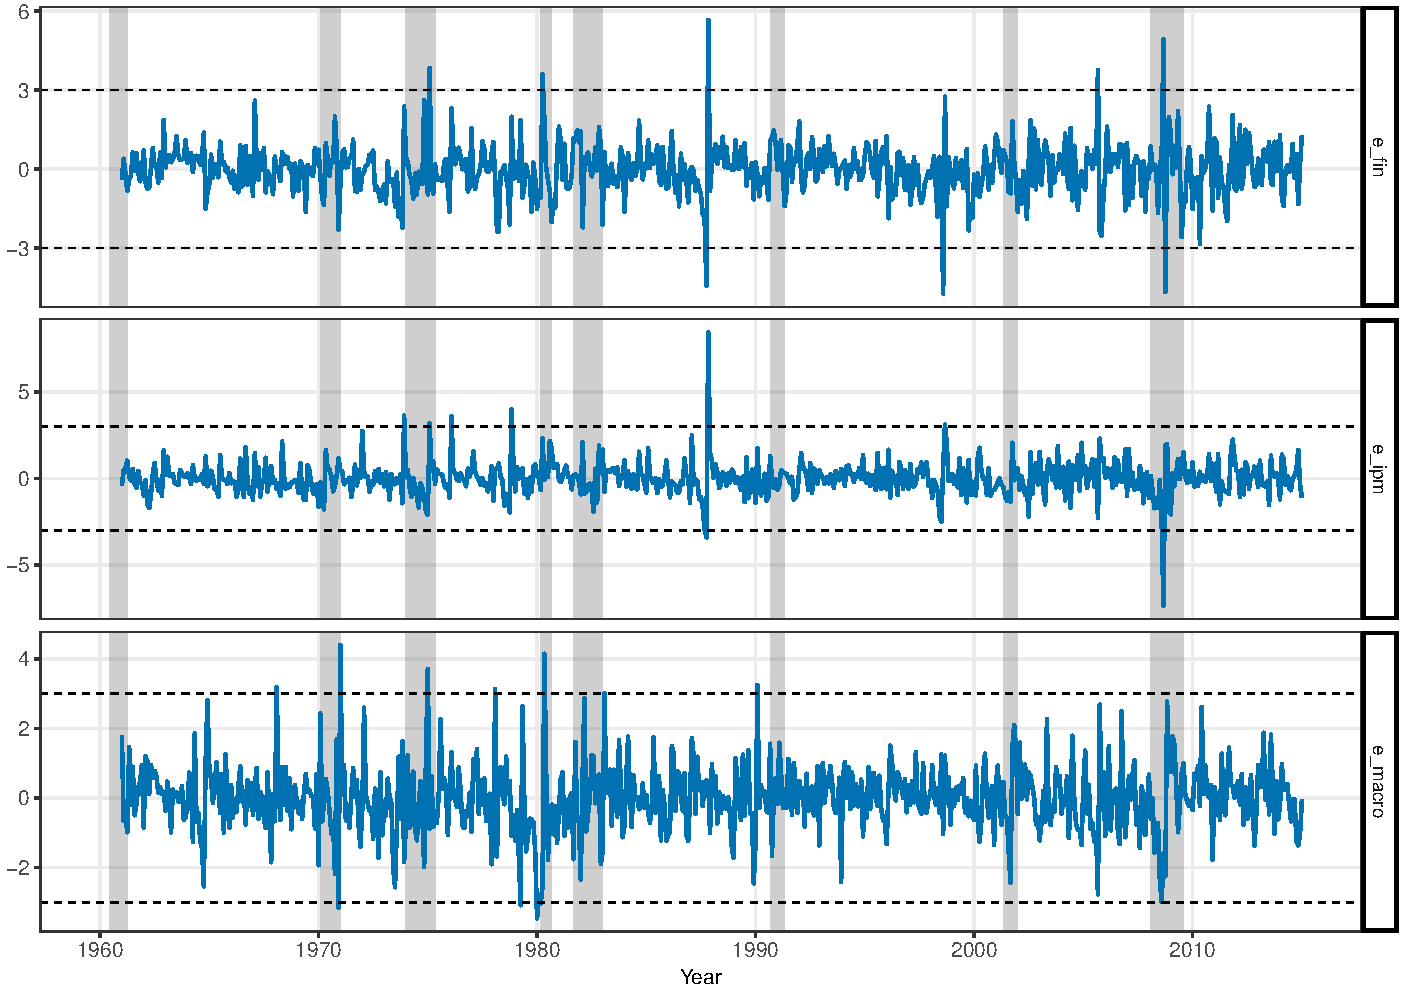
\includegraphics[trim=0.0cm -2.0cm -0.0cm -1cm, width=1\textwidth]{time_series_epsilon_t_maxG.pdf}}
      \caption[Time Series of standardized structural shocks from SVAR ($U_{Macro}, IPM, U_{Fin}$).]{Time Series of standardized structural shocks from SVAR ($U_{Macro}, IPM, U_{Fin}$).\\
      \textit{Note:}  The horizontal line corresponds to 3 standard deviations above/below the unconditional mean of each series. The shocks $\vect{\epsilon}_t = \vect{A}_0\vect{u}_t$ for maxG solution are reported, where $\vect{u}_t$ holds the residuals from VAR(6) of ($U_{Macro}, IPM, U_{Fin}$). The selected bounds are $\overline{\lambda}_1 = -0.05$, $\overline{\lambda}_2 = 2$, $\overline{\lambda}_3 = 0.18$, $\overline{k}_1 = 4$, $\overline{k}_2 = 4$, $\overline{k}_3 = 2$.}   \label{fig:ludvigsonetal_timeseries_e_shocks}
\end{figure}



\begin{figure}[!h]
   \centering
   \setlength\fboxsep{0pt}
   \setlength\fboxrule{0pt}
   \fbox{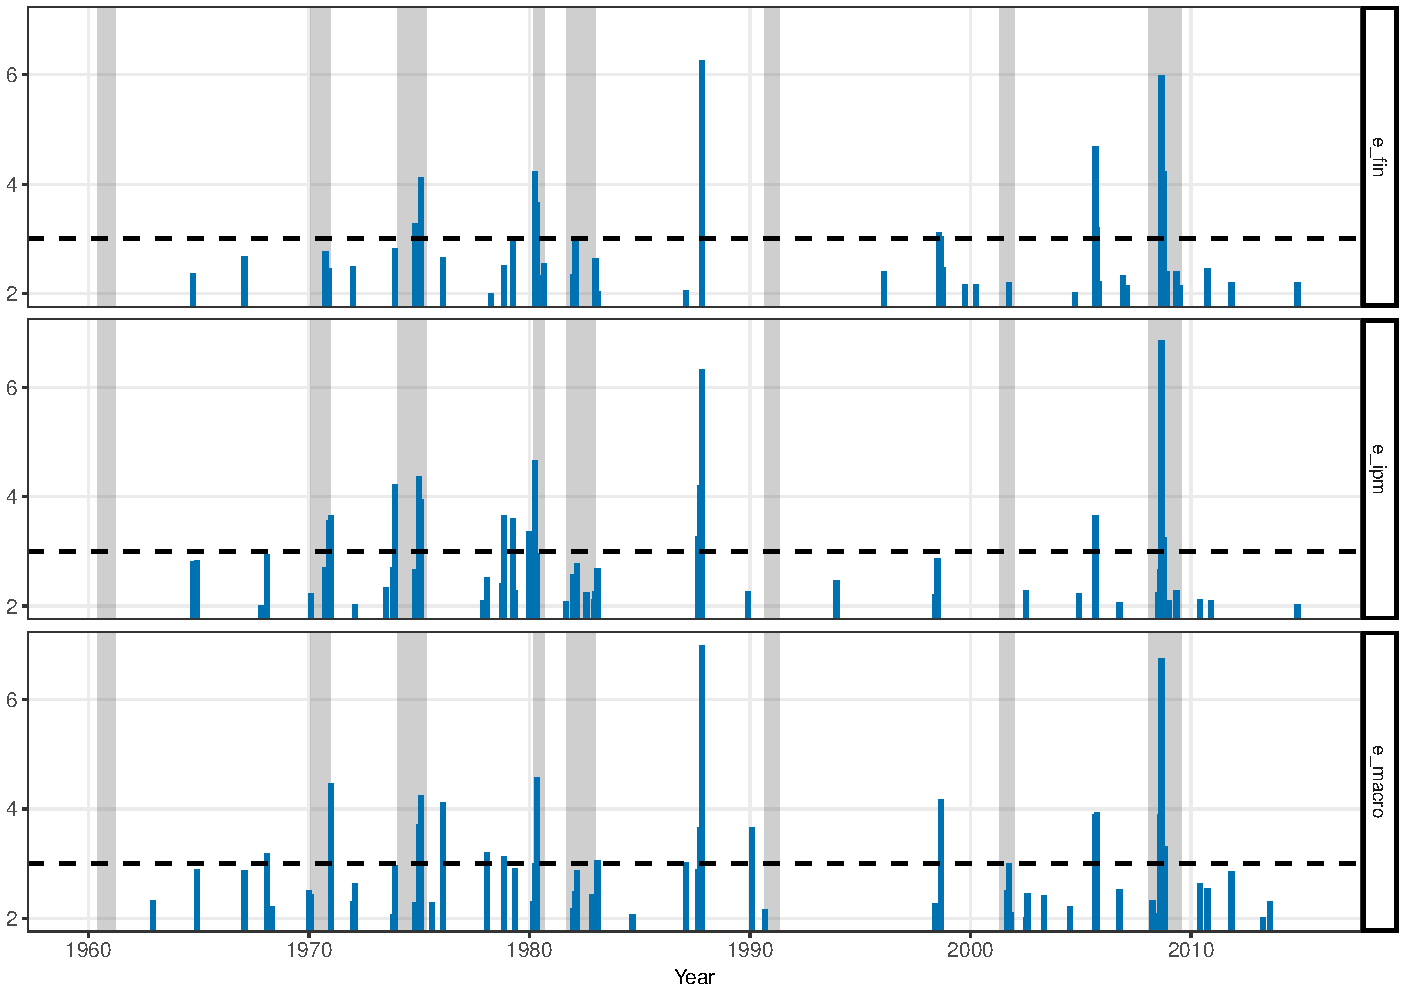
\includegraphics[trim=0.0cm -2.0cm -0.0cm -1cm, width=1\textwidth]{time_series_epsilon_t_largeShocks.pdf}}
      \caption[Large Shocks derived from SVAR ($U_{Macro}, IPM, U_{Fin}$).]{Large Shocks derived from SVAR ($U_{Macro}, IPM, U_{Fin}$).\\
      \textit{Note:}  The figure shows all shocks in the identified set that are at least 2 standard deviations above the unconditional mean for $\epsilon_{Macro}$ and $\epsilon_{Fin}$ and at least 2 standard deviations below the mean for $\epsilon_{ipm}$. For the middle pane ($\epsilon_{ipm}$) the sign of the shocks were flipped (so that negative shocks exceeding 2 standard deviations also point upwards). The horizontal line corresponds to 3 standard deviations. The selected bounds are $\overline{\lambda}_1 = -0.05$, $\overline{\lambda}_2 = 2$, $\overline{\lambda}_3 = 0.18$, $\overline{k}_1 = 4$, $\overline{k}_2 = 4$, $\overline{k}_3 = 2$.}   \label{fig:ludvigsonetal_timeseries_e_largeshocks}
\end{figure}




\section[Impulse Response Analysis]{Impulse Response Analysis}
\label{sec:ImpulseResponseAnalysis}

\begin{figure}[!h]
   \centering
   \setlength\fboxsep{0pt}
   \setlength\fboxrule{0pt}
   \fbox{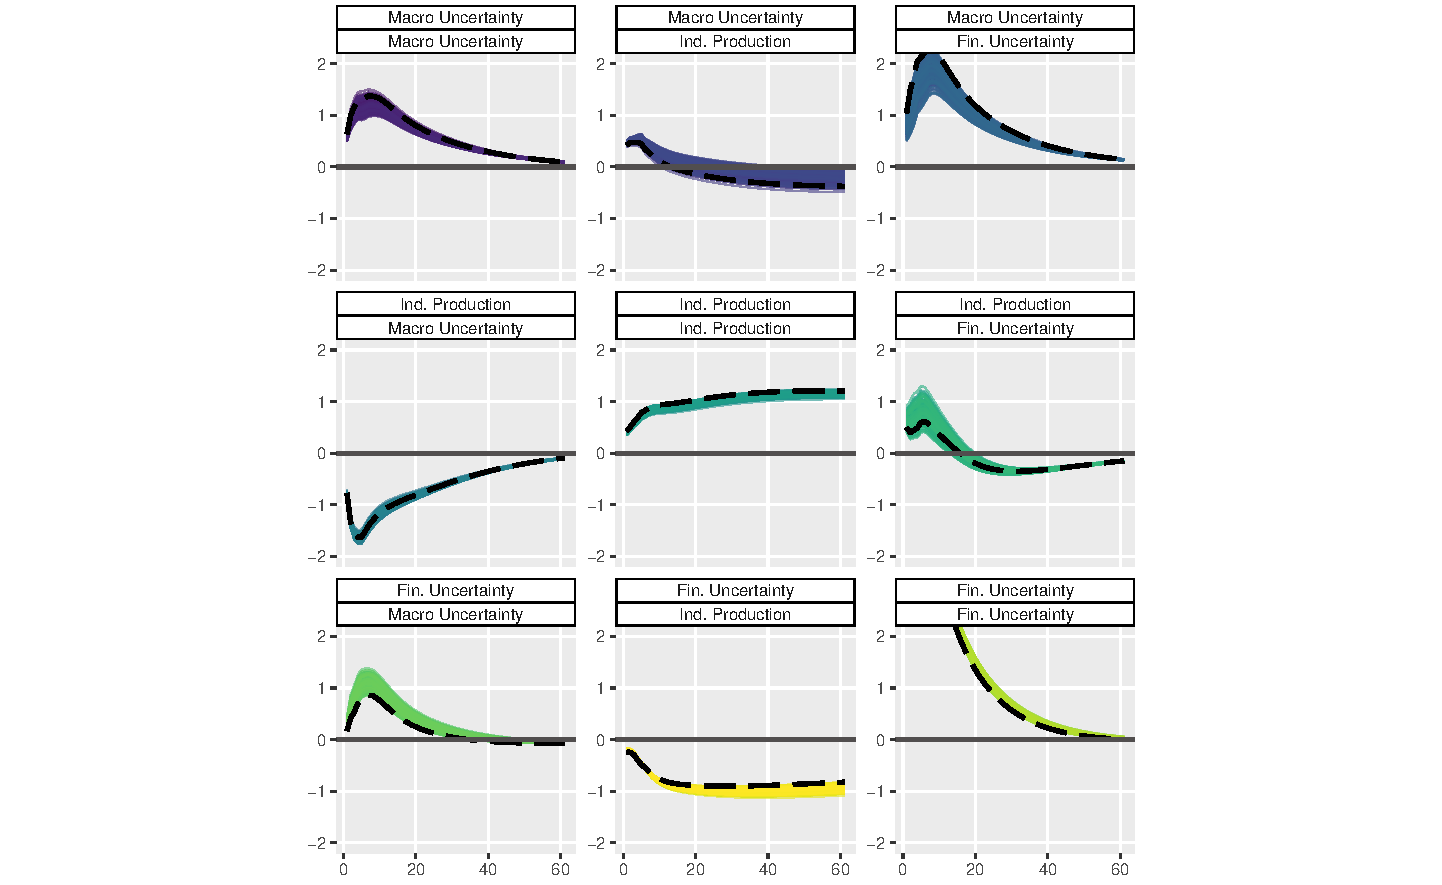
\includegraphics[trim=0.0cm -2.0cm -0.5cm -1cm, width=1\textwidth]{impulse_responses_all_SVAR.pdf}}
      \caption[Impulse Respones from SVAR ($U_{Macro}, IPM, U_{Fin}$).]{Impulse Respones from SVAR ($U_{Macro}, IPM, U_{Fin}$).\\
      \textit{Note:}  The dashed lines are the maxG solutions. The shaded areas represent sets of solutions that satisfy the correlation and event constraints. The selected bounds are $\overline{\lambda}_1 = -0.05$, $\overline{\lambda}_2 = 2$, $\overline{\lambda}_3 = 0.18$, $\overline{k}_1 = 4$, $\overline{k}_2 = 4$, $\overline{k}_3 = 2$.}   \label{fig:impulse.responses_all.SVAR}
\end{figure}

\section[Variance Decomposition]{Variance Decomposition}
\label{sec:VarianceDecomposition}


\chapter{Model Extension}
\label{sec:ModelExtension}

%\newpage
\chapter{Conclusion}
\label{Conclusion}




In the article ``Held Back by Uncertainty'' Bloom and his Colleagues write: '' Policymakers can help.'' --> I should build the conclusion up along these lines! \\
\\
In Kose and Terrones, 2012 (How Does Uncertainty Affect Economic Performance"), p. 5, the authors write: ``Policymakers can do little to alleviate the intrinsic uncertainty economies typically face over the business cycle. However, policy uncertainty is unusually high, and it contributes significantly to macroeconomic uncertainty. By implementing bold and timely measures, policymakers can reduce policy-induced uncertainty and help kick-start economic growth. What precisely policymakers need to do is discussed in the main text of Chapter 1:\\
There, the authors suggest: 
\\
\\
Another problem for VAR-system are omitted variables (which are assumed to be in the innovations). If important variables are omitted from the system, this may lead to major distortions in the impulse responses and makes them worthless for structural interpretations (see Lütkepohl!)


%%%%%%%%%%%%%%%%%%AB HIER ENDET DER INHALT DER ARBEIT%%%%%%%%%%%%%%%%%%%
%%%%%%%%%%%%%%%%%%AB HIER ENDET DER INHALT DER ARBEIT%%%%%%%%%%%%%%%%%%%
%%%%%%%%%%%%%%%%%%AB HIER ENDET DER INHALT DER ARBEIT%%%%%%%%%%%%%%%%%%%
\newpage
\appendix


\chapter{Appendix}
\label{VARAndLocalProjection}
%\section{IRFs in a VAR-Setting}
%\section{IRFs and Local Projections}

\section{Additional Tables}
\label{sec:additionalTables}
\begin{spacing}{.3}
\begin{landscape}
    \centering
    \begin{scriptsize}
    \begin{longtable}{|l|lll|lll|lll|lll|lll|}
    \caption[Comparison of uncertainty measures including shocks following identification methodology of \citet{bloom:09}.]{Comparison of uncertainty measures including shocks following identification methodology of \citet{bloom:09}. \\
    \textit{Note:} High uncertainty periods are defined as periods where a series value is more than 1.65 standard deviations above the HP-detrended mean of the series (\citealp{bloom:09}). Data frequencies are monthly. All series apart from consumer uncertainty series (Michigan Survey) start in July 1962, Michigan Survey in March 1978 and range until June 2008. Column 'ID' marks periods of continuously high uncertainty without interruption (considered a continuous block of 'shocks'), corresponding to an 'ID' the column 'label' marks periods \textit{within} the same 'ID' as either 'f' (first month volatility in a continuous period) or 'm' (maximum volatility in a continuous period) or both (i.e., 'fm').}\\    %%%%<===
\toprule
    \textbf{Date} & \textbf{Michigan} & \textbf{Label} & \textbf{ID} & \textbf{EPU Hist} & \textbf{Label} & \textbf{ID} & \textbf{Macro12} & \textbf{Label} & \textbf{ID} & \textbf{Macro1} & \textbf{Label} & \textbf{ID} & \textbf{VXO} & \textbf{Label} & \textbf{ID} \\ 
    \midrule
    \endhead
       Oct 1962 &  &  &  &  &  &  &  &  &  &  &  &  & 26 & f m & 1 \\
        Nov 1963 &  &  &  &  &  &  &  &  &  &  &  &  & 28.7 & f m & 2 \\
        Aug 1966 &  &  &  &  &  &  &  &  &  &  &  &  & 24.4 & f m & 3 \\
        Oct 1966 &  &  &  &  &  &  &  &  &  &  &  &  & 23.9 & f m & 4 \\
        Jan 1968 &  &  &  & 144 & f m & 1 &  &  &  &  &  &  &  &  &  \\
        Mar 1968 &  &  &  & 123 & f m & 2 &  &  &  &  &  &  &  &  &  \\
        May 1970 &  &  &  &  &  &  &  &  &  &  &  &  & 37.6 & f m & 5 \\
        Nov 1971 &  &  &  & 154 & f m & 3 &  &  &  &  &  &  &  &  &  \\
        Jul 1973 &  &  &  &  &  &  & 1.02 & f  & 1 &  &  &  &  &  &  \\
        Aug 1973 &  &  &  &  &  &  & 1.04 &   & 1 & 0.79 & f  & 1 &  &  &  \\
        Sep 1973 &  &  &  &  &  &  & 1.04 &   & 1 & 8$\times10^{-1}$ &   & 1 &  &  &  \\
        Oct 1973 &  &  &  &  &  &  & 1.04 &   & 1 & 8$\times10^{-1}$ &  m & 1 &  &  &  \\
        Nov 1973 &  &  &  &  &  &  & 1.04 &   & 1 & 0.79 &   & 1 & 28.8 & f  & 6 \\
        Dec 1973 &  &  &  &  &  &  & 1.03 &   & 1 & 0.79 &   & 1 & 34.1 &  m & 6 \\
        Jan 1974 &  &  &  & 160 & f m & 4 & 1.03 &   & 1 & 8$\times10^{-1}$ &   & 1 &  &  &  \\
        Feb 1974 &  &  &  &  &  &  & 1.03 &   & 1 &  &  &  &  &  &  \\
        Mar 1974 &  &  &  &  &  &  & 1.03 &   & 1 &  &  &  &  &  &  \\
        Apr 1974 &  &  &  &  &  &  & 1.03 &   & 1 & 0.79 & f m & 2 &  &  &  \\
        May 1974 &  &  &  &  &  &  & 1.04 &   & 1 &  &  &  &  &  &  \\
        Jun 1974 &  &  &  &  &  &  & 1.04 &   & 1 &  &  &  &  &  &  \\
        Jul 1974 &  &  &  &  &  &  & 1.05 &   & 1 & 8$\times10^{-1}$ & f  & 3 & 29.8 & f  & 7 \\
        Aug 1974 &  &  &  &  &  &  & 1.06 &   & 1 & 0.82 &   & 3 & 29.2 &   & 7 \\
        Sep 1974 &  &  &  &  &  &  & 1.06 &   & 1 & 0.82 &   & 3 & 36.8 &   & 7 \\
        Oct 1974 &  &  &  &  &  &  & 1.06 &   & 1 & 0.83 &   & 3 & 38.4 &  m & 7 \\
        Nov 1974 &  &  &  &  &  &  & 1.06 &  m & 1 & 0.85 &   & 3 &  &  &  \\
        Dec 1974 &  &  &  & 162 & f m & 5 & 1.06 &   & 1 & 0.87 &  m & 3 &  &  &  \\
        Jan 1975 &  &  &  &  &  &  & 1.04 &   & 1 & 0.84 &   & 3 &  &  &  \\
        Feb 1975 &  &  &  &  &  &  & 1.03 &   & 1 & 0.82 &   & 3 &  &  &  \\
        Mar 1975 &  &  &  &  &  &  &  &  &  & 8$\times10^{-1}$ &   & 3 &  &  &  \\
        Jul 1979 &  &  &  & 175 & f m & 6 &  &  &  &  &  &  &  &  &  \\
        Jan 1980 &  &  &  &  &  &  & 1.12 & f  & 2 &  &  &  &  &  &  \\
        Feb 1980 &  &  &  &  &  &  & 1.15 &   & 2 & 9$\times10^{-1}$ & f  & 4 &  &  &  \\
        Mar 1980 &  &  &  &  &  &  & 1.18 &   & 2 & 0.95 &   & 4 & 29.2 & f m & 8 \\
        Apr 1980 &  &  &  &  &  &  & 1.21 &  m & 2 & 1 &  m & 4 &  &  &  \\
        May 1980 &  &  &  &  &  &  & 1.21 &   & 2 & 0.98 &   & 4 &  &  &  \\
        Jun 1980 &  &  &  &  &  &  & 1.2 &   & 2 & 0.95 &   & 4 &  &  &  \\
        Jul 1980 &  &  &  &  &  &  & 1.18 &   & 2 & 0.95 &   & 4 &  &  &  \\
        Aug 1980 &  &  &  &  &  &  & 1.17 &   & 2 & 0.93 &   & 4 &  &  &  \\
        Sep 1980 &  &  &  &  &  &  & 1.16 &   & 2 & 0.91 &   & 4 &  &  &  \\
        Oct 1980 &  &  &  &  &  &  & 1.15 &   & 2 & 9$\times10^{-1}$ &   & 4 &  &  &  \\
        Nov 1980 &  &  &  &  &  &  & 1.15 &   & 2 & 0.89 &   & 4 &  &  &  \\
        Dec 1980 &  &  &  &  &  &  & 1.16 &   & 2 & 0.89 &   & 4 &  &  &  \\
        Jan 1981 &  &  &  &  &  &  & 1.16 &   & 2 & 0.89 &   & 4 &  &  &  \\
        Feb 1981 &  &  &  &  &  &  & 1.16 &   & 2 & 0.88 &   & 4 &  &  &  \\
        Mar 1981 &  &  &  &  &  &  & 1.15 &   & 2 &  &  &  &  &  &  \\
        Apr 1981 &  &  &  &  &  &  & 1.15 &   & 2 &  &  &  &  &  &  \\
        May 1981 &  &  &  &  &  &  & 1.14 &   & 2 &  &  &  &  &  &  \\
        Jun 1981 &  &  &  &  &  &  & 1.15 &   & 2 &  &  &  &  &  &  \\
        Jul 1981 &  &  &  &  &  &  & 1.14 &   & 2 &  &  &  &  &  &  \\
        Aug 1981 &  &  &  &  &  &  & 1.13 &   & 2 &  &  &  &  &  &  \\
        Sep 1981 &  &  &  &  &  &  & 1.13 &   & 2 &  &  &  &  &  &  \\
        Oct 1981 &  &  &  &  &  &  & 1.13 &   & 2 &  &  &  &  &  &  \\
        Nov 1981 &  &  &  &  &  &  & 1.12 &   & 2 &  &  &  &  &  &  \\
        Jan 1982 &  &  &  &  &  &  &  &  &  & 0.88 & f  & 5 &  &  &  \\
        Feb 1982 &  &  &  &  &  &  &  &  &  & 0.88 &  m & 5 &  &  &  \\
        Aug 1982 &  &  &  &  &  &  &  &  &  &  &  &  & 32.4 & f m & 9 \\
        Oct 1982 &  &  &  &  &  &  &  &  &  &  &  &  & 32.8 & f m & 10 \\
        Nov 1982 &  &  &  &  &  &  &  &  &  &  &  &  & 32.4 &   & 10 \\
        Jan 1986 &  &  &  & 202 & f m & 7 &  &  &  &  &  &  &  &  &  \\
        Oct 1987 &  &  &  & 236 & f m & 8 &  &  &  &  &  &  & 58.2 & f m & 11 \\
        Nov 1987 &  &  &  & 227 &   & 8 &  &  &  &  &  &  & 49.4 &   & 11 \\
        Dec 1987 & 5 & f m & 1 & 197 &   & 8 &  &  &  &  &  &  & 41.8 &   & 11 \\
        Jan 1988 & 5 &  m & 1 &  &  &  &  &  &  &  &  &  & 38.3 &   & 11 \\
        Feb 1988 &  &  &  &  &  &  &  &  &  &  &  &  & 33.7 &   & 11 \\
        Sep 1990 &  &  &  & 195 & f m & 9 &  &  &  &  &  &  & 28.8 & f  & 12 \\
        Oct 1990 &  &  &  &  &  &  &  &  &  &  &  &  & 30.1 &  m & 12 \\
        Nov 1990 & 8.33 & f  & 2 & 190 & f m & 10 &  &  &  &  &  &  &  &  &  \\
        Dec 1990 & 11 &   & 2 &  &  &  &  &  &  &  &  &  &  &  &  \\
        Jan 1991 & 11.7 &  m & 2 & 242 & f m & 11 &  &  &  &  &  &  &  &  &  \\
        Feb 1991 & 11.7 &  m & 2 &  &  &  &  &  &  &  &  &  &  &  &  \\
        Mar 1991 & 8.67 &   & 2 &  &  &  &  &  &  &  &  &  &  &  &  \\
        Dec 1991 & 8 & f  & 3 & 220 & f m & 12 &  &  &  &  &  &  &  &  &  \\
        Jan 1992 & 10 &   & 3 &  &  &  &  &  &  &  &  &  &  &  &  \\
        Feb 1992 & 10.3 &   & 3 & 190 & f m & 13 &  &  &  &  &  &  &  &  &  \\
        Mar 1992 & 11 &  m & 3 &  &  &  &  &  &  &  &  &  &  &  &  \\
        Apr 1992 & 9.67 &   & 3 &  &  &  &  &  &  &  &  &  &  &  &  \\
        May 1992 & 8.33 &   & 3 &  &  &  &  &  &  &  &  &  &  &  &  \\
        Aug 1992 & 8.33 & f  & 4 &  &  &  &  &  &  &  &  &  &  &  &  \\
        Sep 1992 & 9.33 &   & 4 &  &  &  &  &  &  &  &  &  &  &  &  \\
        Oct 1992 & 9.67 &  m & 4 & 204 & f m & 14 &  &  &  &  &  &  &  &  &  \\
        Nov 1992 & 8 &   & 4 &  &  &  &  &  &  &  &  &  &  &  &  \\
        Nov 1997 &  &  &  &  &  &  &  &  &  &  &  &  & 31.5 & f m & 13 \\
        Aug 1998 &  &  &  & 176 & f  & 15 &  &  &  &  &  &  &  &  &  \\
        Sep 1998 &  &  &  & 216 &  m & 15 &  &  &  &  &  &  & 39.2 & f m & 14 \\
        Oct 1998 &  &  &  & 193 &   & 15 &  &  &  &  &  &  & 37.5 &   & 14 \\
        Nov 2000 &  &  &  & 221 & f m & 16 &  &  &  &  &  &  &  &  &  \\
        Dec 2000 &  &  &  & 2$\times10^{2}$ &   & 16 &  &  &  &  &  &  &  &  &  \\
        Jun 2001 & 5.33 & f m & 5 &  &  &  &  &  &  &  &  &  &  &  &  \\
        Sep 2001 & 5.33 & f  & 6 & 313 & f m & 17 &  &  &  & 0.78 & f  & 6 & 42.7 & f m & 15 \\
        Oct 2001 & 7 &   & 6 & 288 &   & 17 &  &  &  & 0.79 &  m & 6 & 34.5 &   & 15 \\
        Nov 2001 & 8 &  m & 6 & 215 &   & 17 &  &  &  & 0.76 &   & 6 &  &  &  \\
        Dec 2001 & 6 &   & 6 &  &  &  &  &  &  &  &  &  &  &  &  \\
        Jan 2002 &  &  &  & 197 & f m & 18 &  &  &  &  &  &  &  &  &  \\
        Jul 2002 &  &  &  &  &  &  &  &  &  &  &  &  & 38.5 & f  & 16 \\
        Aug 2002 &  &  &  &  &  &  &  &  &  &  &  &  & 37.2 &   & 16 \\
        Sep 2002 &  &  &  &  &  &  &  &  &  &  &  &  & 41.7 &  m & 16 \\
        Oct 2002 &  &  &  &  &  &  &  &  &  &  &  &  & 41.4 &   & 16 \\
        Nov 2002 &  &  &  & 2$\times10^{2}$ & f m & 19 &  &  &  &  &  &  &  &  &  \\
        Jan 2003 &  &  &  & 230 & f m & 20 &  &  &  &  &  &  &  &  &  \\
        Feb 2003 & 5.67 & f  & 7 &  &  &  &  &  &  &  &  &  & 36.5 & f m & 17 \\
        Mar 2003 & 6.67 &  m & 7 & 250 & f m & 21 &  &  &  &  &  &  & 35.2 &   & 17 \\
        Apr 2003 & 6.33 &   & 7 & 207 &   & 21 &  &  &  &  &  &  &  &  &  \\
        May 2003 & 5.67 &   & 7 &  &  &  &  &  &  &  &  &  &  &  &  \\
        Aug 2007 &  &  &  &  &  &  &  &  &  &  &  &  & 25.1 & f m & 18 \\
        Nov 2007 &  &  &  &  &  &  &  &  &  &  &  &  & 26.7 & f m & 19 \\
        Jan 2008 &  &  &  & 240 & f m & 22 &  &  &  &  &  &  & 28 & f  & 20 \\
        Feb 2008 &  &  &  &  &  &  &  &  &  &  &  &  & 27.2 &   & 20 \\
        Mar 2008 &  &  &  &  &  &  &  &  &  &  &  &  & 29 &  m & 20 \\
        Apr 2008 & 7 & f  & 8 &  &  &  &  &  &  &  &  &  &  &  &  \\
        May 2008 & 7.33 &  m & 8 &  &  &  &  &  &  & 8$\times10^{-1}$ & f  & 7 &  &  &  \\
        Jun 2008 & 6.67 &   & 8 &  &  &  & 1.04 & f m & 3 & 0.83 &  m & 7 &  &  &  \\
        \bottomrule
        \end{longtable}
\end{scriptsize}
\end{landscape}
\label{tab:tab_bloom_shock_all}
\end{spacing}


\begin{spacing}{.3}
\begin{landscape}
    \centering
    \begin{scriptsize}
    \begin{longtable}{|l|lll|lll|lll|lll|lll|}
    \caption[Comparison of uncertainty measures including shocks following identification methodology of \citet{bloom:09}.]{Comparison of uncertainty measures including shocks following identification methodology of \citet{bloom:09}. \\
    \textit{Note:} High uncertainty periods are defined as periods where a series value is more than 1.65 standard deviations above the HP-detrended mean of the series (\citealp{bloom:09}). Data frequencies are monthly. All series apart from consumer uncertainty series (Michigan Survey) start in July 1962, Michigan Survey in March 1978 and range until June 2008. Column 'ID' marks periods of continuously high uncertainty without interruption (considered a continuous block of 'shocks'), corresponding to an 'ID' the column 'label' marks periods \textit{within} the same 'ID' as either 'f' (first month volatility in a continuous period) or 'm' (maximum volatility in a continuous period) or both (i.e., 'fm').}\\    %%%%<===
\toprule
    \textbf{Date} & \textbf{Michigan} & \textbf{Label} & \textbf{ID} & \textbf{EPU Hist} & \textbf{Label} & \textbf{ID} & \textbf{Macro12} & \textbf{Label} & \textbf{ID} & \textbf{Macro1} & \textbf{Label} & \textbf{ID} & \textbf{VXO} & \textbf{Label} & \textbf{ID} \\ 
    \midrule
    \endhead
        Oct 1962 &  &  &  &  &  &  &  &  &  &  &  &  & 26 & f m & 1 \\
        Nov 1963 &  &  &  &  &  &  &  &  &  &  &  &  & 28.7 & f m & 2 \\
        Aug 1966 &  &  &  &  &  &  &  &  &  &  &  &  & 24.4 & f m & 3 \\
        Jan 1968 &  &  &  & 144 & f m & 1 &  &  &  &  &  &  &  &  &  \\
        Mar 1968 &  &  &  & 123 & f m & 2 &  &  &  &  &  &  &  &  &  \\
        May 1970 &  &  &  &  &  &  &  &  &  &  &  &  & 37.6 & f m & 4 \\
        Nov 1971 &  &  &  & 154 & f m & 3 &  &  &  &  &  &  &  &  &  \\
        Aug 1973 &  &  &  &  &  &  & 1.04 & f  & 1 &  &  &  &  &  &  \\
        Sep 1973 &  &  &  &  &  &  & 1.04 &   & 1 &  &  &  &  &  &  \\
        Oct 1973 &  &  &  &  &  &  & 1.04 &   & 1 & 8$\times10^{-1}$ & f m & 1 &  &  &  \\
        Nov 1973 &  &  &  &  &  &  & 1.04 &   & 1 &  &  &  &  &  &  \\
        Dec 1973 &  &  &  &  &  &  & 1.03 &   & 1 &  &  &  & 34.1 & f m & 5 \\
        Jan 1974 &  &  &  &  &  &  & 1.03 &   & 1 &  &  &  &  &  &  \\
        Feb 1974 &  &  &  &  &  &  & 1.03 &   & 1 &  &  &  &  &  &  \\
        Mar 1974 &  &  &  &  &  &  & 1.03 &   & 1 &  &  &  &  &  &  \\
        Apr 1974 &  &  &  &  &  &  & 1.03 &   & 1 &  &  &  &  &  &  \\
        May 1974 &  &  &  &  &  &  & 1.04 &   & 1 &  &  &  &  &  &  \\
        Jun 1974 &  &  &  &  &  &  & 1.04 &   & 1 &  &  &  &  &  &  \\
        Jul 1974 &  &  &  &  &  &  & 1.05 &   & 1 &  &  &  &  &  &  \\
        Aug 1974 &  &  &  &  &  &  & 1.06 &   & 1 & 0.82 & f  & 2 &  &  &  \\
        Sep 1974 &  &  &  &  &  &  & 1.06 &   & 1 & 0.82 &   & 2 & 36.8 & f  & 6 \\
        Oct 1974 &  &  &  &  &  &  & 1.06 &   & 1 & 0.83 &   & 2 & 38.4 &  m & 6 \\
        Nov 1974 &  &  &  &  &  &  & 1.06 &  m & 1 & 0.85 &   & 2 &  &  &  \\
        Dec 1974 &  &  &  &  &  &  & 1.06 &   & 1 & 0.87 &  m & 2 &  &  &  \\
        Jan 1975 &  &  &  &  &  &  & 1.04 &   & 1 & 0.84 &   & 2 &  &  &  \\
        Feb 1975 &  &  &  &  &  &  & 1.03 &   & 1 & 0.82 &   & 2 &  &  &  \\
        Jul 1979 &  &  &  & 175 & f m & 4 &  &  &  &  &  &  &  &  &  \\
        Jan 1980 &  &  &  &  &  &  & 1.12 & f  & 2 &  &  &  &  &  &  \\
        Feb 1980 &  &  &  &  &  &  & 1.15 &   & 2 & 9$\times10^{-1}$ & f  & 3 &  &  &  \\
        Mar 1980 &  &  &  &  &  &  & 1.18 &   & 2 & 0.95 &   & 3 & 29.2 & f m & 7 \\
        Apr 1980 &  &  &  &  &  &  & 1.21 &  m & 2 & 1 &  m & 3 &  &  &  \\
        May 1980 &  &  &  &  &  &  & 1.21 &   & 2 & 0.98 &   & 3 &  &  &  \\
        Jun 1980 &  &  &  &  &  &  & 1.2 &   & 2 & 0.95 &   & 3 &  &  &  \\
        Jul 1980 &  &  &  &  &  &  & 1.18 &   & 2 & 0.95 &   & 3 &  &  &  \\
        Aug 1980 &  &  &  &  &  &  & 1.17 &   & 2 & 0.93 &   & 3 &  &  &  \\
        Sep 1980 &  &  &  &  &  &  & 1.16 &   & 2 & 0.91 &   & 3 &  &  &  \\
        Oct 1980 &  &  &  &  &  &  & 1.15 &   & 2 & 9$\times10^{-1}$ &   & 3 &  &  &  \\
        Nov 1980 &  &  &  &  &  &  & 1.15 &   & 2 & 0.89 &   & 3 &  &  &  \\
        Dec 1980 &  &  &  &  &  &  & 1.16 &   & 2 &  &  &  &  &  &  \\
        Jan 1981 &  &  &  &  &  &  & 1.16 &   & 2 &  &  &  &  &  &  \\
        Feb 1981 &  &  &  &  &  &  & 1.16 &   & 2 &  &  &  &  &  &  \\
        Mar 1981 &  &  &  &  &  &  & 1.15 &   & 2 &  &  &  &  &  &  \\
        Apr 1981 &  &  &  &  &  &  & 1.15 &   & 2 &  &  &  &  &  &  \\
        May 1981 &  &  &  &  &  &  & 1.14 &   & 2 &  &  &  &  &  &  \\
        Jun 1981 &  &  &  &  &  &  & 1.15 &   & 2 &  &  &  &  &  &  \\
        Jul 1981 &  &  &  &  &  &  & 1.14 &   & 2 &  &  &  &  &  &  \\
        Aug 1981 &  &  &  &  &  &  & 1.13 &   & 2 &  &  &  &  &  &  \\
        Sep 1981 &  &  &  &  &  &  & 1.13 &   & 2 &  &  &  &  &  &  \\
        Oct 1981 &  &  &  &  &  &  & 1.13 &   & 2 &  &  &  &  &  &  \\
        Nov 1981 &  &  &  &  &  &  & 1.12 &   & 2 &  &  &  &  &  &  \\
        Feb 1982 &  &  &  &  &  &  &  &  &  & 0.88 & f m & 4 &  &  &  \\
        Aug 1982 &  &  &  &  &  &  &  &  &  &  &  &  & 32.4 & f m & 8 \\
        Oct 1982 &  &  &  &  &  &  &  &  &  &  &  &  & 32.8 & f m & 9 \\
        Nov 1982 &  &  &  &  &  &  &  &  &  &  &  &  & 32.4 &   & 9 \\
        Jan 1986 &  &  &  & 202 & f m & 5 &  &  &  &  &  &  &  &  &  \\
        Oct 1987 &  &  &  & 236 & f m & 6 &  &  &  &  &  &  & 58.2 & f m & 10 \\
        Nov 1987 &  &  &  & 227 &   & 6 &  &  &  &  &  &  & 49.4 &   & 10 \\
        Dec 1987 & 5 & f m & 1 & 197 &   & 6 &  &  &  &  &  &  & 41.8 &   & 10 \\
        Jan 1988 & 5 &  m & 1 &  &  &  &  &  &  &  &  &  & 38.3 &   & 10 \\
        Feb 1988 &  &  &  &  &  &  &  &  &  &  &  &  & 33.7 &   & 10 \\
        Sep 1990 &  &  &  & 195 & f m & 7 &  &  &  &  &  &  &  &  &  \\
        Oct 1990 &  &  &  &  &  &  &  &  &  &  &  &  & 30.1 & f m & 11 \\
        Nov 1990 & 8.33 & f  & 2 &  &  &  &  &  &  &  &  &  &  &  &  \\
        Dec 1990 & 11 &   & 2 &  &  &  &  &  &  &  &  &  &  &  &  \\
        Jan 1991 & 11.7 &  m & 2 & 242 & f m & 8 &  &  &  &  &  &  &  &  &  \\
        Feb 1991 & 11.7 &  m & 2 &  &  &  &  &  &  &  &  &  &  &  &  \\
        Mar 1991 & 8.67 &   & 2 &  &  &  &  &  &  &  &  &  &  &  &  \\
        Dec 1991 & 8 & f  & 3 & 220 & f m & 9 &  &  &  &  &  &  &  &  &  \\
        Jan 1992 & 10 &   & 3 &  &  &  &  &  &  &  &  &  &  &  &  \\
        Feb 1992 & 10.3 &   & 3 &  &  &  &  &  &  &  &  &  &  &  &  \\
        Mar 1992 & 11 &  m & 3 &  &  &  &  &  &  &  &  &  &  &  &  \\
        Apr 1992 & 9.67 &   & 3 &  &  &  &  &  &  &  &  &  &  &  &  \\
        May 1992 & 8.33 &   & 3 &  &  &  &  &  &  &  &  &  &  &  &  \\
        Aug 1992 & 8.33 & f  & 4 &  &  &  &  &  &  &  &  &  &  &  &  \\
        Sep 1992 & 9.33 &   & 4 &  &  &  &  &  &  &  &  &  &  &  &  \\
        Oct 1992 & 9.67 &  m & 4 & 204 & f m & 10 &  &  &  &  &  &  &  &  &  \\
        Nov 1992 & 8 &   & 4 &  &  &  &  &  &  &  &  &  &  &  &  \\
        Sep 1998 &  &  &  & 216 & f m & 11 &  &  &  &  &  &  & 39.2 & f m & 12 \\
        Oct 1998 &  &  &  & 193 &   & 11 &  &  &  &  &  &  & 37.5 &   & 12 \\
        Nov 2000 &  &  &  & 221 & f m & 12 &  &  &  &  &  &  &  &  &  \\
        Dec 2000 &  &  &  & 2$\times10^{2}$ &   & 12 &  &  &  &  &  &  &  &  &  \\
        Apr 2001 & 5 & f m & 5 &  &  &  &  &  &  &  &  &  &  &  &  \\
        Jun 2001 & 5.33 & f m & 6 &  &  &  &  &  &  &  &  &  &  &  &  \\
        Sep 2001 & 5.33 & f  & 7 & 313 & f m & 13 &  &  &  & 0.78 & f  & 5 & 42.7 & f m & 13 \\
        Oct 2001 & 7 &   & 7 & 288 &   & 13 &  &  &  & 0.79 &  m & 5 &  &  &  \\
        Nov 2001 & 8 &  m & 7 & 215 &   & 13 &  &  &  & 0.76 &   & 5 &  &  &  \\
        Dec 2001 & 6 &   & 7 &  &  &  &  &  &  &  &  &  &  &  &  \\
        Jul 2002 &  &  &  &  &  &  &  &  &  &  &  &  & 38.5 & f  & 14 \\
        Aug 2002 &  &  &  &  &  &  &  &  &  &  &  &  & 37.2 &   & 14 \\
        Sep 2002 &  &  &  &  &  &  &  &  &  &  &  &  & 41.7 &  m & 14 \\
        Oct 2002 &  &  &  &  &  &  &  &  &  &  &  &  & 41.4 &   & 14 \\
        Nov 2002 &  &  &  & 2$\times10^{2}$ & f m & 14 &  &  &  &  &  &  &  &  &  \\
        Jan 2003 &  &  &  & 230 & f m & 15 &  &  &  &  &  &  &  &  &  \\
        Feb 2003 & 5.67 & f  & 8 &  &  &  &  &  &  &  &  &  & 36.5 & f m & 15 \\
        Mar 2003 & 6.67 &  m & 8 & 250 & f m & 16 &  &  &  &  &  &  & 35.2 &   & 15 \\
        Apr 2003 & 6.33 &   & 8 & 207 &   & 16 &  &  &  &  &  &  &  &  &  \\
        May 2003 & 5.67 &   & 8 &  &  &  &  &  &  &  &  &  &  &  &  \\
        Jan 2008 &  &  &  & 240 & f m & 17 &  &  &  &  &  &  &  &  &  \\
        Jul 2008 &  &  &  &  &  &  & 1.06 & f  & 3 & 0.87 & f  & 6 &  &  &  \\
        Aug 2008 &  &  &  &  &  &  & 1.09 &   & 3 & 0.93 &   & 6 &  &  &  \\
        Sep 2008 &  &  &  & 275 & f  & 18 & 1.12 &   & 3 & 1 &   & 6 &  &  &  \\
        Oct 2008 &  &  &  & 297 &  m & 18 & 1.15 &   & 3 & 1.06 &  m & 6 & 65.5 & f m & 16 \\
        Nov 2008 & 9.33 & f  & 9 & 222 &   & 18 & 1.15 &  m & 3 & 1.06 &   & 6 & 65.4 &   & 16 \\
        Dec 2008 & 10 &   & 9 &  &  &  & 1.15 &   & 3 & 1.04 &   & 6 & 55 &   & 16 \\
        Jan 2009 & 9.67 &   & 9 & 237 & f m & 19 & 1.13 &   & 3 & 1.03 &   & 6 & 44.3 &   & 16 \\
        Feb 2009 & 10 &   & 9 & 234 &   & 19 & 1.11 &   & 3 & 0.99 &   & 6 & 45.4 &   & 16 \\
        Mar 2009 & 11.3 &  m & 9 &  &  &  & 1.09 &   & 3 & 0.94 &   & 6 & 46.1 &   & 16 \\
        Apr 2009 & 11.3 &  m & 9 &  &  &  & 1.07 &   & 3 & 0.91 &   & 6 & 38.9 &   & 16 \\
        May 2009 & 9.67 &   & 9 &  &  &  & 1.06 &   & 3 & 0.89 &   & 6 &  &  &  \\
        Jun 2009 &  &  &  &  &  &  & 1.04 &   & 3 & 0.88 &   & 6 &  &  &  \\
        Jul 2009 &  &  &  &  &  &  &  &  &  & 0.85 &   & 6 &  &  &  \\
        Jul 2010 &  &  &  & 245 & f m & 20 &  &  &  &  &  &  &  &  &  \\
        Sep 2010 &  &  &  & 241 & f m & 21 &  &  &  &  &  &  &  &  &  \\
        Jul 2011 &  &  &  & 256 & f  & 22 &  &  &  &  &  &  &  &  &  \\
        Aug 2011 &  &  &  & 351 &  m & 22 &  &  &  &  &  &  & 35.1 & f  & 17 \\
        Sep 2011 &  &  &  & 259 &   & 22 &  &  &  &  &  &  & 36.6 &  m & 17 \\
        Oct 2011 & 10.7 & f m & 10 &  &  &  &  &  &  &  &  &  & 32 &   & 17 \\
        Nov 2011 & 10.7 &  m & 10 &  &  &  &  &  &  &  &  &  & 31.4 &   & 17 \\
        Dec 2011 &  &  &  & 237 & f m & 23 &  &  &  &  &  &  &  &  &  \\
        Nov 2012 &  &  &  & 251 & f  & 24 &  &  &  &  &  &  &  &  &  \\
        Dec 2012 &  &  &  & 251 &  m & 24 &  &  &  &  &  &  &  &  &  \\
        Jan 2013 &  &  &  & 248 &   & 24 &  &  &  &  &  &  &  &  &  \\
        Oct 2013 &  &  &  & 287 & f m & 25 &  &  &  &  &  &  &  &  &  \\
        Sep 2015 &  &  &  &  &  &  &  &  &  &  &  &  & 24.6 & f m & 18 \\
        Jan 2016 &  &  &  &  &  &  &  &  &  &  &  &  & 24.3 & f m & 19 \\
        Feb 2016 &  &  &  &  &  &  &  &  &  &  &  &  & 24.1 &   & 19 \\
        \bottomrule
        \end{longtable}
\end{scriptsize}
\end{landscape}
\label{tab:tab_bloom_shock_all_until2016}
\end{spacing}


\begin{spacing}{.9}
\begin{landscape}
\centering
    \begin{longtable}{rrrrllrr}
    \caption[Major Stock-Market Volatility Shocks following \citet{bloom:09}.]{Major Stock-Market Volatility Shocks. Replication of Table A.1 in \citet{bloom:09}.} \\
    \toprule
         ID & Date Begin & Date End & Duration & Max Vol & First Vol & Date Max Vol & Date First Vol \\ \midrule
         1 & Oct 1962 & Oct 1962 & 1 & 26 & 26 & Oct 1962 & Oct 1962 \\
         2 & Nov 1963 & Nov 1963 & 1 & 28.7 & 28.7 & Nov 1963 & Nov 1963 \\
         3 & Aug 1966 & Aug 1966 & 1 & 24.4 & 24.4 & Aug 1966 & Aug 1966 \\
         4 & Oct 1966 & Oct 1966 & 1 & 23.9 & 23.9 & Oct 1966 & Oct 1966 \\
         5 & May 1970 & May 1970 & 1 & 37.6 & 37.6 & May 1970 & May 1970 \\
         6 & Nov 1973 & Dec 1973 & 2 & 34.1 & 28.8 & Dec 1973 & Nov 1973 \\
         7 & Jul 1974 & Oct 1974 & 4 & 38.4 & 29.8 & Oct 1974 & Jul 1974 \\
         8 & Mar 1980 & Mar 1980 & 1 & 29.2 & 29.2 & Mar 1980 & Mar 1980 \\
         9 & Aug 1982 & Aug 1982 & 1 & 32.4 & 32.4 & Aug 1982 & Aug 1982 \\
        10 & Oct 1982 & Nov 1982 & 2 & 32.8 & 32.8 & Oct 1982 & Oct 1982 \\
        11 & Oct 1987 & Feb 1988 & 5 & 49.4 & 40.8 & Nov 1987 & Oct 1987 \\
        12 & Aug 1990 & Oct 1990 & 3 & 30.1 & 27.8 & Oct 1990 & Aug 1990 \\
        13 & Jan 1991 & Jan 1991 & 1 & 26.9 & 26.9 & Jan 1991 & Jan 1991 \\
        14 & Nov 1997 & Nov 1997 & 1 & 31.6 & 31.6 & Nov 1997 & Nov 1997 \\
        15 & Sep 1998 & Oct 1998 & 2 & 39.2 & 39.2 & Sep 1998 & Sep 1998 \\
        16 & Sep 2001 & Oct 2001 & 2 & 42.6 & 42.6 & Sep 2001 & Sep 2001 \\
        17 & Jul 2002 & Oct 2002 & 4 & 41.7 & 38.5 & Sep 2002 & Jul 2002 \\
        18 & Feb 2003 & Mar 2003 & 2 & 36.5 & 36.5 & Feb 2003 & Feb 2003 \\
        19 & Aug 2007 & Aug 2007 & 1 & 25.1 & 25.1 & Aug 2007 & Aug 2007 \\
        20 & Nov 2007 & Nov 2007 & 1 & 26.7 & 26.7 & Nov 2007 & Nov 2007 \\
        21 & Jan 2008 & Mar 2008 & 3 & 29 & 28.1 & Mar 2008 & Jan 2008 \\
\bottomrule
        \end{longtable}
\end{landscape}
\label{tab:bloom_shocks}
\end{spacing}


\section{Additional Figures}
\begin{landscape}
\begin{figure}[!t]
   \centering
   \setlength\fboxsep{0pt}
   \setlength\fboxrule{0pt}
   \fbox{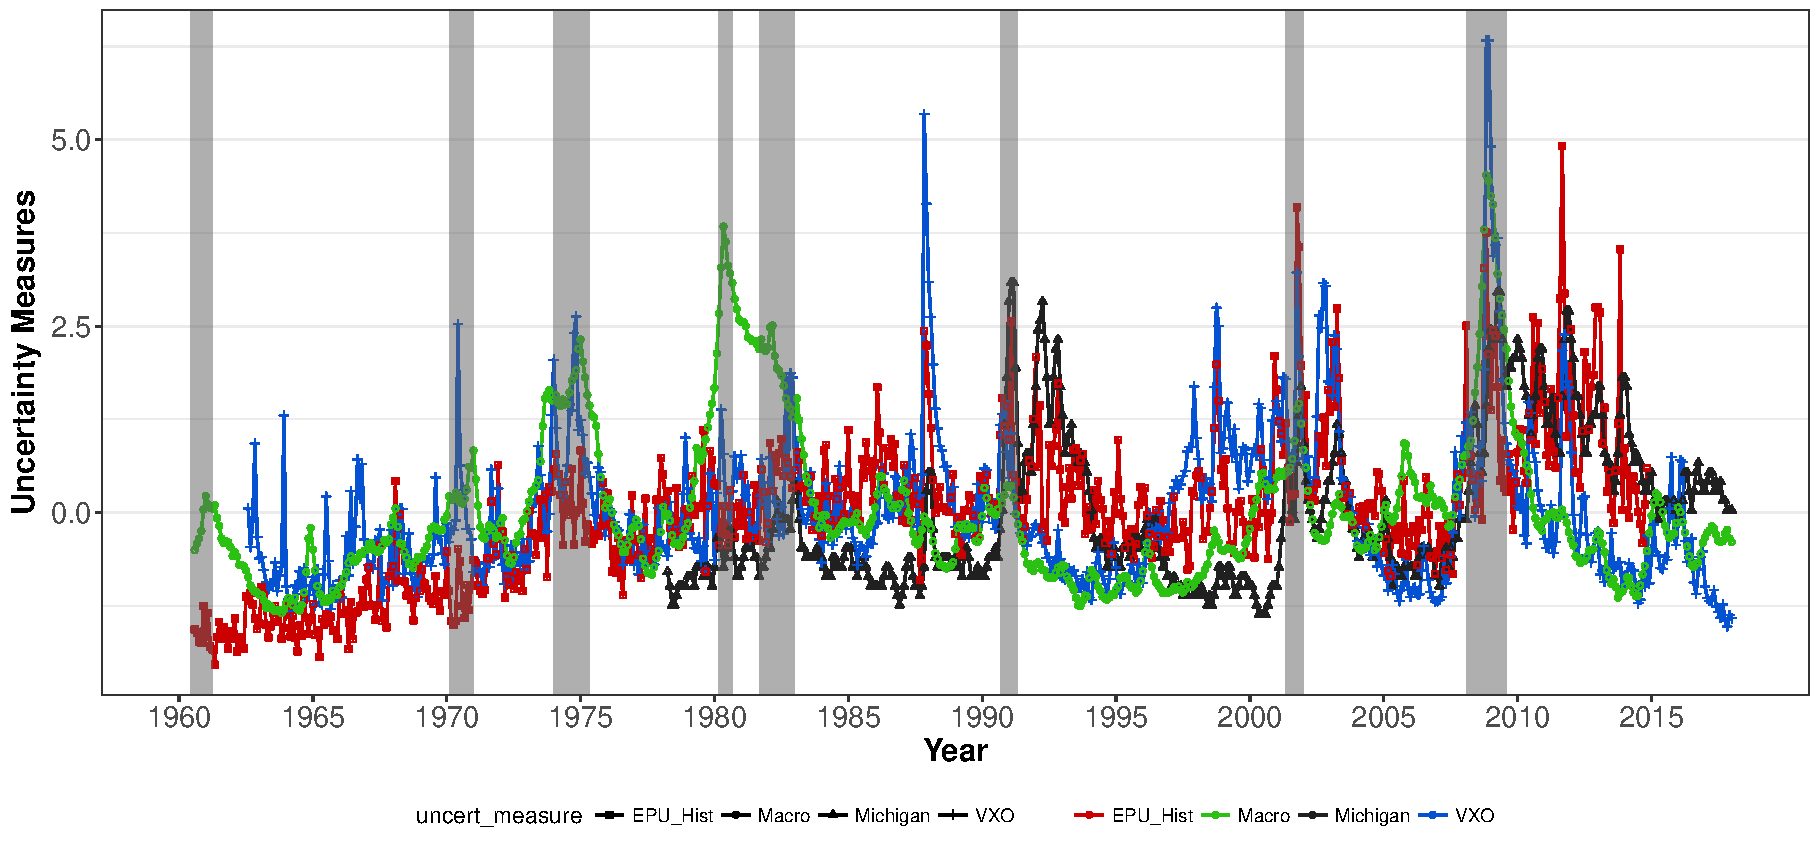
\includegraphics[trim=1cm -0.8cm 0.8cm 0.2cm, width=1.5\textwidth]{comparison_plot_combined.pdf}}
      \caption[Comparison of uncertainty measures (combined).]{Comparison of uncertainty measures (facetted).
      \textit{Note:} Shaded areas denote NBER recession dates in the US. Data frequencies are monthly. The macro uncertainty series starts in July 1960, the GTU in January 2004, the EPU in January 1985, the consumer uncertainty series in January 1978  and the VXO in July 1962.}   \label{fig:comparison_plot_combined}
\end{figure}
\end{landscape}



\begin{landscape}
\begin{figure}[!t]
   \centering
   \setlength\fboxsep{0pt}
   \setlength\fboxrule{0pt}
   \fbox{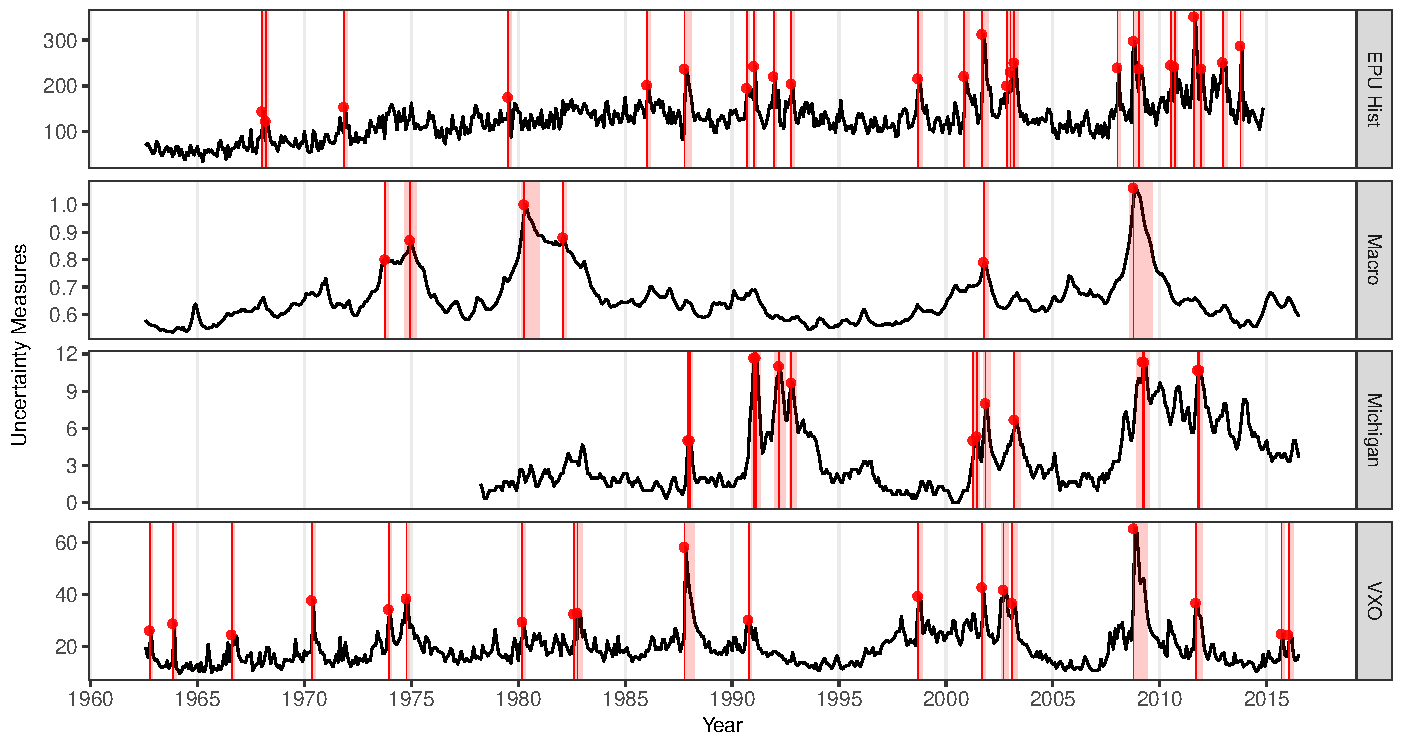
\includegraphics[trim=1cm -0.8cm 0.8cm 0.2cm, width=1.5\textwidth]{BLOOM_Shocks_plot_combined_all2016.pdf}}
      \caption[Comparison of uncertainty measures (combined).]{Comparison of uncertainty measures (facetted).
      \textit{Note:} Shaded areas denote NBER recession dates in the US. Data frequencies are monthly. The macro uncertainty series starts in July 1960, the GTU in January 2004, the EPU in January 1985, the consumer uncertainty series in January 1978  and the VXO in July 1962.}   \label{fig:bloom_shock_all_until2016}
\end{figure}
\end{landscape}



\section{Additional VAR Results}




\chapter{Appendix}
\label{DataAndCode}
\section{Data: Sources and Description}
\label{sec:data}
Table~\ref{tab:data_sources} lists all data and their sources that appear in the main text. Variables that enter the VAR and/or Local Projection estimations in Section~\ref{sec:EmpiricalAnalysis} are listed below.


\paragraph{Monthly VAR-8 following \citet{bloom:09}} Endogenous variables, in order:\\
Then we create separate explanations about which variables were used for which model:\\

\begingroup
\begin{spacing}{0.5}
    \fontsize{10pt}{12pt}\selectfont
\begin{enumerate}
	\item log($\text{S\&P500}_t$)
	\item uncertainty (various measures)
	\item $\text{FFR}_t$
	\item log($\text{WAGE}_t$)
	\item log($\text{CPI}_t$)
	\item log($\text{HOURS}_t$)
	\item log($\text{EMPM}_t$)	
	\item log($\text{IP}_t$)		
\end{enumerate}
\end{spacing}
\endgroup



\paragraph{Monthly VAR-11 following \citet{juradoetal:15}} Endogenous variables, in order:\\
Then we create separate explanations about which variables were used for which model:\\

\begingroup
\begin{spacing}{0.5}
    \fontsize{10pt}{12pt}\selectfont
\begin{enumerate}
	\item log($\text{IP}_t$)
	\item log($\text{EMPM}_t$)
	\item log(real consumption --> still to be added! download from IHS!
	\item log($\text{PCE deflator}_t$) --> still to be added! download from IHS!
	\item log($\text{NO}_t$ $=$ $\text{NO capital}_t$ $+$ $\text{NO cons}_t$) --> two components to be added! download from IHS!
	\item log($\text{WAGE}_t$)
	\item log($\text{HOURS}_t$)
	\item $\text{FFR}_t$
	\item log($\text{S\&P500}_t$)
	\item growth rate of $\text{M2}_t$
	\item uncertainty (various measures)
\end{enumerate}
\end{spacing}
\endgroup


\paragraph{Local Projections \citep{jorda:05}}


\begin{table}[!h]
\caption[Data Sources.]{Data Sources.\\
\textit{Note:} Federal Reserve Economic Data (FRED); Chicago Board Options Exchange (CBOE); Michigan Survey of Consumers (MSoC); }
\renewcommand{\arraystretch}{1.5}
\resizebox{\textwidth}{!}{%
\centering % used for centering table
% note: the letter 'p' helps to vertically align all rows (even if one row has more text than others!)
\begin{tabular}{L{2.7cm}p{5.4cm}p{2.5cm}p{3.4cm}L{2.5cm}} % centered columns (4 columns)
\toprule
         Variable & Name &  Source & Code & Period \\ 
         \midrule
        $\text{IP}_t$ & Industrial Production Index (Monthly, Seasonally Adjusted) & FRED & INDPRO & 1962M07- \\
        $\text{EMPM}_t$ & All Employees: Manufacturing (Monthly, Seasonally Adjusted) & FRED & MANEMP & 1962M07- \\
                $\text{HOURS}_t$ & Average Weekly Hours of Production and Nonsupervisory Employees: Manufacturing (Monthly, Seasonally Adjusted) & FRED & AWHMAN & 1962M07- \\
         $\text{CPI}_t$ & Consumer Price Index for All Urban Consumers: All Items (Monthly, Seasonally Adjusted) & FRED & CPIAUSCSL & 1962M07- \\
 	$\text{NO capital}_t$ & Value of Manufacturers' New Orders for Capital Goods: Nondefense Capital Goods Industries (Monthly, Seasonally Adjusted) & IHS & M_178554409  & 1962M07- \\
 	$\text{NO cons}_t$ & Value of Manufacturers' New Orders for Capital Goods: Nondefense Capital Goods Industries (Monthly, Seasonally Adjusted) & IHS & M_14385863 & 1962M07- \\
         $\text{WAGE}_t$ & Average Hourly Earnings of Production and Nonsupervisory Employees: Manufacturing (Monthly, Seasonally Adjusted) & FRED & AHEMAN & 1962M07- \\
           $\text{M2}_t$ & M" Money Stock (Monthly, Seasonally Adjusted) & FRED & M2SL & 1962M07- \\
         $\text{FFR}_t$ & Effective Federal Funds Rate & FRED & FEDFUNDS & 1962M07- \\
         $\text{S\&P500}_t$ & S\&P's Common Stock Price Index: Composite (Monthly) & YAHOO Finance & S\&P 500 (^GSPC) & 1962M07- \\
         $\text{VXO}_t$ & Cboe S\&P 100 Volatility Index - VXO & CBOE & VXO & 1986M01- \\
         $\text{Michigan}_t$ & Consumer Uncertainty (Michigan Survey of Consumers) & MSoC & veh_fb_unc & 1978M03- \\
 	$\text{Macro1/3/12}_t$ & Macro Uncertainty Index & \citet{juradoetal:15}\footnote{Downloaded from \url{https://www.sydneyludvigson.com/data-and-appendixes}.} &  & 1962M07- \\
	$\text{EPU}_t$ & Economic Policy Uncertainty Index & \citet{bakeretal:15}\footnote{Downloaded from \url{http://www.policyuncertainty.com/}.} & News Based Policy Uncert Index & 1962M07- \\
	$\text{EPU Historical}_t$ & Economic Policy Uncertainty Index & \citet{bakeretal:15}\footnote{Downloaded from \url{http://www.policyuncertainty.com/}.} & News-Based Historical Economic Policy Uncertainty & 1962M07- \\
        \bottomrule
\end{tabular}
}
\label{tab:data_sources} % is used to refer this table in the text
\end{table}




\newgeometry{left=25mm, right=25mm, top=30mm, bottom=30mm}
%the below code is to adjust the header ruler after the
%newgeometry!
\fancyhfoffset[E,O]{0pt}
\section{Code}
\label{sec:rcode}
%\begin{Verbatim}[fontsize=\small]
%halloe
%\end{Verbatim} 

%\begin{verbatim}
%halloe
%\end{verbatim} 

\begingroup
\fontsize{9pt}{12pt}\selectfont
\begin{verbatim}  
##The Code will go here.




\end{verbatim}  
\endgroup


\restoregeometry

%%%%%%%%%%%%%%%%%%%%%%%%%BIBLIOGRAPHY%%%%%%%%%%%%%%%%%%%%%%%%%%%%
%%%%%%%%%%%%%%%%%%%%%%%%%BIBLIOGRAPHY%%%%%%%%%%%%%%%%%%%%%%%%%%%%
%%%%%%%%%%%%%%%%%%%%%%%%%BIBLIOGRAPHY%%%%%%%%%%%%%%%%%%%%%%%%%%%%

\nocite{*}
\clearpage
\thispagestyle{empty}
\bibliographystyle{agsm}
%bibliographystyle{agsm} bewirkt, dass KEINE Beistriche zwischen den Jahreszahlen sind. Dafür aber
%Gänsefüßchen beim Titel der Werke!
\bibliography{mybiblio}





%%%%%%%%%%%%%%%%%%%%%%EIDESSTATTLICHE ERKLÄRUNG%%%%%%%%%%%%%%%%%%%%%%
\clearpage
\thispagestyle{empty}
\null\vspace{46pt}
\paragraph{\large{Declaration of Authorship}}
\vspace{43pt}
I hereby declare that I prepared this master's thesis independently and that the thoughts taken
directly or indirectly from other sources are acknowledged as references accordingly. \\
\\
The work contained in this thesis has neither been previously submitted to any other examination authority nor published in any other form which has led to the award of a degree.\\[10mm]

    Innsbruck, \makebox[1.8in][l]{\hrulefill} \qquad \makebox[2.6in]{\hrulefill}\\
    \makebox[2.95in][l]      \hfill\makebox[2.0in][l]{(Signature: Marcel Kropp)}

\clearpage
\thispagestyle{empty}
\null\vspace{46pt}
\paragraph{\large{Eidesstattliche Erklärung}}
\vspace{43pt}
Ich erkläre hiermit an Eides Statt, dass ich dir vorliegende Masterarbeit selbständig angefertig habe. Die aus fremden Quellen direkt oder indirekt übernommenen Gedanken sind als solche kenntlich gemacht. \\
\\
Die Arbeit wurde bisher weder in gleicher noch in ähnlicher Form einer anderen Prüfungsbehörde vorgelegt und auch noch nicht veröffentlicht.\\[10mm]

    Innsbruck, \makebox[1.8in][l]{\hrulefill} \qquad \makebox[2.6in]{\hrulefill}\\
    \makebox[2.95in][l]      \hfill\makebox[2.0in][l]{(Unterschrift: Marcel Kropp)}


%%%%%%%%%%%%%%%%%%%%%%EIDESSTATTLICHE ERKLÄRUNG%%%%%%%%%%%%%%%%%%%%%%

\end{document}
%%%%%%%%%%%%%%%%%%%%%%END OF THE DOCUMENT%%%%%%%%%%%%%%%%%%%%%%%%%%
%%%%%%%%%%%%%%%%%%%%%%END OF THE DOCUMENT%%%%%%%%%%%%%%%%%%%%%%%%%%
%%%%%%%%%%%%%%%%%%%%%%END OF THE DOCUMENT%%%%%%%%%%%%%%%%%%%%%%%%%%